%% LyX 2.3.1 created this file.  For more info, see http://www.lyx.org/.
%% Do not edit unless you really know what you are doing.
\documentclass[english]{report}
\usepackage[T1]{fontenc}
\setcounter{secnumdepth}{5}
\setcounter{tocdepth}{3}
\usepackage{babel}
\usepackage{varioref}
\usepackage{makeidx}
\makeindex
\usepackage{graphicx}

\makeatletter

%%%%%%%%%%%%%%%%%%%%%%%%%%%%%% LyX specific LaTeX commands.
%% Because html converters don't know tabularnewline


%%%%%%%%%%%%%%%%%%%%%%%%%%%%%% Textclass specific LaTeX commands.
\newenvironment{lyxcode}
	       {
<lyxcode>
               }
	       {
</lyxcode>
}

%%%%%%%%%%%%%%%%%%%%%%%%%%%%%% User specified LaTeX commands.
\usepackage{a4wide}
\usepackage{times}

\makeatother

\begin{document}
\newcommand{\bold}[1]{{\bf #1}}

This is the MQL Programmer's Guide. It documents Emdros version 3.7.0
and upwards. If you just wish to use Emdros to query your data, then
this might not be for you. Instead, you can consult the MQL Query
Guide, which is available from the Emdros website, or with any recent
distribution of Emdros.

In Chapter 1, we discuss some preliminaries, such as the history of
Emdros, as well as giving an overview of the formalism used to define
the MQL language, called Backus-Naur Form (or BNF).

In Chapter 2, we give an overview of the EMdF model, from a user's
standpoint.

In Chapter 3, we describe the bulk of the MQL language.

In Chapter 4, we describe the query-subset of MQL. That is, the subset
of MQL in which you can express queries that look for objects by object
type, features, and structural relationships such as embedding and
sequence.

\chapter{Preliminaries}

\section{Introduction}

Welcome to the MQL Programmer's Guide. MQL is the query
language associated with the EMdF model. MQL is
a ``full access language,'' which simply
means that MQL lets you create, update, delete, and query most of
the data domains in the EMdF model -- databases,
objects, object types, features, etc. MQL is your front-end to the
EMdF database engine. This guide helps
you formulate MQL queries that do what you need done with your EMdF
database.

This guide has four chapters. The first is this chapter on preliminaries.
The second is a gentle introduction to the EMdF model,
which underlies the MQL language. The third chapter deals with the
bulk of the MQL query language, detailing all the different kinds
of queries for creating, updating, deleting, and querying an EMdF
database. The fourth chapter is a special chapter
devoted to explaining those MQL queries that query for objects in
the database. Since these queries are so rich, it was deemed necessary
to devote a whole chapter to their treatment.

This chapter will proceed as follows. First, we present a short
history of MdF, EMdF, and MQL. Second, we give a gentle introduction
to Backus-Naur Form, or BNF, which will be used throughout chapters 3
and 4. Lastly, we explain the origin of the support for something
called \emph{regular expressions} in MQL. This is done so as to comply
with the license for the library used.

But first, an explanation of where EMdF and MQL come from.

\section{Origins of MdF, EMdF, and MQL}

EMdF and MQL are not original works. They are merely derivative works
based on someone else's hard labors. Most of the ideas underlying
the EMdF model and the MQL query language are to be found in the PhD
thesis of Crist-Jan Doedens, published
in 1994 as \cite{Doedens94}. This thesis described, among other things,
the MdF database model and the QL query language. As one
might guess, EMdF stems from MdF, and MQL stems from QL.

The EMdF model takes over the MdF model in its entirety, but adds
a few concepts which are useful when implementing the MdF model in
real life. Thus the `E' in `EMdF' stands for ``Extended'', yielding
the ``Extended MdF model''. The EMdF model
is the subject of chapter 2.

``MQL'' stands for ``Mini QL.'' Originally,
I devised MQL as a subset of the QL query language developed
in Dr. Doedens' PhD thesis, hence the ``Mini''
modifier. Since then, however, MQL has grown. QL was not
a full access language, but specified
only how to query an MdF database, i.e., how to ask questions of it.
MQL, by contrast, is a full access language,
allowing not only querying, but also creation, update, and deletion
of the data domains of the EMdF model. The MQL
query language is the subject of chapters 3
and 4.

Thus EMdF and MQL are derivatives of the MdF database model and the
QL query language developed by Dr. Crist-Jan Doedens in his 1994 PhD
thesis.

\section{Introduction to Backus-Naur Form}

\subsection{Context-Free Grammars}

BNF is a way of specifying the ``syntactic rules'' of a language.
English also has ``syntactic rules,'' and some of them can be specified
using a ``Context-Free Grammar.'' BNF is precisely a way of specifying
a context-free grammar for a formal language. Thus it is beneficial
first to see what a context-free grammar is, before looking at the
details of BNF.

In English, the basic clause-pattern is ``Subject - Verb - Object''.
For example, in the clause ``I eat vegetables,'' the word ``I''
is the subject, the word ``eat'' is the verb, and the word ``vegetables''
is the object. A clause which exhibits exactly the same ``Subject
- Verb - Object'' structure is ``You drink coke.'' Here, ``You''
is the subject, ``drink'' is the verb, and ``coke'' is the object.

Consider the following context-free grammar:


\begin{lyxcode}
Sentence~$\rightarrow$~NP$_{subj}$~VP

NP$_{subj}$~$\rightarrow$~``I''~|~``You''

VP~$\rightarrow$~V~NP$_{obj}$

V~$\rightarrow$~``eat''~|~``drink''

NP$_{obj}$~$\rightarrow$~``vegetables''~|~``coke''
\end{lyxcode}

This little context-free grammar is a toy example of a context-free
grammar. However, despite its simplicity, it exemplifies all of the
concepts involved in context-free grammars:
\begin{itemize}
\item Rule
\item Non-terminal
\item Terminal
\item Choice
\item Concatenation
\item Start-symbol.
\end{itemize}
These will be described in turn below

\subsubsection{Rule}

A ``Rule'' consists of three parts:
\begin{enumerate}
\item The left-hand side
\item The ``production arrow'' (``$\rightarrow$'').
\item The right-hand side
\end{enumerate}

An example of a rule in the above context-free grammar is:

\begin{lyxcode}
Sentence~$\rightarrow$~NP$_{subj}$~VP
\end{lyxcode}

It specifies that the left-hand side (``Sentence'') can be \emph{replaced
with} the right-hand side, which in this case is two symbols, ``NP$_{subj}$''
followed by ``VP''. Sometimes, we also say that a left-hand side
is \emph{expanded to} the right-hand side.

\subsubsection{Non-terminal}

There are only two kinds of symbols in a context-free grammar: Non-terminals
and Terminals. They are a contrasting pair. In this section, we describe
what a non-terminal is, and in the next section, what a terminal is.

A ``Non-terminal'' is a symbol in a rule which can be expanded to
other symbols. Thus the symbols ``Sentence'', ``NP$_{subj}$'',
``VP'', ``V'', and ``NP$_{obj}$'' constitute all of the non-terminals
of the above context-free grammar. 

Only non-terminals can stand on the left-hand side of a rule. A non-terminal
is defined as a symbol which can be expanded to or replaced with other
symbols, and hence they can stand on the left-hand side of a rule.
But as you will notice in the above context-free grammar, a non-terminal
can also stand on the right-hand-side of a rule. For example, the
non-terminal ``V'' is present both in the rule for how to expand
the non-terminal ``VP'', and in the rule for how to expand itself.
Thus, in order to expand ``VP'' fully, you must first expand to
the right-hand-side ``V NP$_{obj}$'', and then expand both ``V''
and ``NP$_{obj}$'', using the rules for these two.

\subsubsection{Terminal}

A ``Terminal'' is a symbol in a rule which cannot be expanded to
other symbols. Hence, it is ``terminal'' in the sense that the expansion
cannot proceed further from this symbol. In the above context-free
grammar, the terminals are: ``I'', ``You'', ``eat'', ``drink'',
``vegetables'', and ``coke''. These are symbols which cannot be
expanded further. 

Terminals can only stand on the right-hand side of a rule. If they
were to stand on the left-hand-side of the rule, that would mean that
they could be expanded to or replaced with other symbols. But that
would make them non-terminals.

\subsubsection{Choice}

In the rule for ``V'' in the above grammar, we see an example of
choice. The choice is indicated by the ``|'' symbol, which is read
as ``or''. Thus, this example:

\begin{lyxcode}
V~$\rightarrow$~``eat''~|~``drink''
\end{lyxcode}

is read as `V expands to ``eat'' \emph{or} ``drink'''.

\subsubsection{Concatenation}

We have already seen an example of concatenation, namely in the rule
for ``Sentence'':

Sentence $\rightarrow$ NP$_{subj}$ VP

Here, the symbols ``NP$_{subj}$'' and ``VP'' are \emph{concatenated},
or placed in sequence. Thus ``VP'' comes immediately after ``NP$_{subj}$''. 

``Concatenated'' is simply a fanciful name for ``being in sequence'',
but although it is a basic idea, we included it for completeness.

\subsubsection{Start-symbol}

The start-symbol is merely the left-hand side non-terminal of the
first rule in the grammar. Thus, in the above grammar, ``Sentence''
is the start-symbol.

\subsection{Context-free grammars: Putting it all together}

It is time to see how all of this theory works in practice. The above
grammar can produce 8 sentences, some of which do not make sense:
\begin{enumerate}
\item I eat vegetables
\item I eat coke
\item I drink vegetables
\item I drink coke
\item You eat vegetables
\item You eat coke
\item You drink vegetables
\item You drink coke
\end{enumerate}
Let us pick one of these sentences and see how it was produced from
the above grammar. We will pick number 8, ``You drink coke'', and
trace all the steps. We start with the start-symbol, ``Sentence'':
\begin{enumerate}
\item Sentence

This is expanded using the rule for ``Sentence'':
\item NP$_{subj}$ VP

The ``NP$_{subj}$'' non-terminal is then expanded to ``You''
using one of the choices in the rule for NP$_{subj}$:
\item ``You'' VP

The ``VP'' is then expanded using the rule for ``VP'':
\item ``You'' V NP$_{obj}$

The ``V'' non-terminal is then expanded to the terminal ``drink'':
\item ``You'' ``drink'' NP$_{obj}$

The ``NP$_{obj}$'' non-terminal is then expanded to the terminal
``coke'':
\item ``You'' ``drink'' ``coke''

Which yields the final sentence, ``You drink coke''. This sentence
has no non-terminals, only terminals, and therefore it cannot be expanded
further. We are finished.
\end{enumerate}
If you would like to, try to trace the production of one of the other
sentences using pencil and paper, tracing each step as in the above
example. When you have done so once or twice, you should understand
all there is to understand about context-free grammars.

And BNF is simply a way of specifying a context-free grammar. So let
us start looking at the details of BNF.

\subsection{BNF}

\subsubsection{Introduction}

BNF comes in various variants, and almost everyone defines their usage
of BNF a little differently from everyone else. In this document,
we shall also deviate slightly from ``standard BNF'', but these
deviations will only be very slight.

This treatment of BNF will be made from an example of a context-free
grammar in ``MQL BNF.'' This example covers every formalism used
in ``MQL BNF,'' and is a real-life example of the syntax of an actual
MQL statement:

\subsubsection{Example}

\begin{lyxcode}
create\_enumeration\_statement~:~``CREATE''~

~~~~~~~~~~~~(``ENUMERATION''~|~``ENUM'')~

~~~~~~~~~~~~enumeration\_name~``=''~

~~~~~~~~~~~~``\{''~ec\_declaration\_list~``\}''

;

enumeration\_name~:~T\_IDENTIFIER

~~~/{*}~The~T\_IDENTIFIER~is~a~terminal~

~~~~~~denoting~an~identifier.~{*}/

;

ec\_declaration\_list~:~ec\_declaration~\{~``,''~ec\_declaration~\}

;

ec\_declaration~:~{[}~``DEFAULT''~{]}

~~~~~~~~~~~~~~ec\_name~{[}~ec\_initialization~{]}

;

ec\_name~:~T\_IDENTIFIER

;

ec\_initialization~:~``=''~T\_INTEGER

;
\end{lyxcode}

\subsubsection{Elements of ``MQL BNF''}

All of the elements of ``MQL BNF'' can be listed as follows:
\begin{enumerate}
\item Rule

This is just the same as in the context-free grammars above, except
that the ``$\rightarrow$'' production arrow is replaced by a ``:``
colon. Also, a rule ends with a ``;'' semicolon.
\item Non-terminal

Non-terminals always start with a lower-case letter, e.g., ``ec\_declaration.''
\item Terminal

Terminals are either strings in ``double quotes'' or strings that
start with ``T\_'', e.g., ``T\_IDENTIFIER''.
\item Choice

This is the same as in the context-free grammars. The symbol ``|''
is used.
\item Concatenation

This is the same as in the context-free grammars. A space between
two symbols is used.
\item Start-symbol

This is the same as in the context-free grammars. The left-hand side
non-terminal of the first rule is the start-symbol.
\item Comment

A comment is enclosed in /{*} slashes and stars {*}/. The comments
are not part of the grammar, but serve to explain a part of the grammar
to the human reader.
\item Optional specification

A symbol or sequence of symbols enclosed in {[}square brackets{]}
is considered optional. For example, the \texttt{ec\_initialization}
non-terminal is optional in the \texttt{ec\_declaration} rule. Both
terminals and non-terminals can be optional. Here, the choice is between
``ENUM'' and ``ENUMERATION'', rather than, say, ``CREATE ENUMERATION''
and the rest of the rule.
\item Bracketing

Sometimes, we do not go to the trouble of spelling out a choice with
a rule by itself. Instead, (brackets) are used. For example, in the
above grammar, there is a choice between ``ENUMERATION'' and ``ENUM''.
Only one must be chosen when writing the CREATE ENUMERATION statement.
The brackets serve to let you know the scope of the choice, i.e.,
between exactly which elements the choice stands.
\item Bracing (repetition)

The \{ braces \} are used to indicate that the enclosed part can be
repeated zero or more times. For example, in the rule for \texttt{ec\_declaration\_list},
the first \texttt{ec\_declaration} can be followed by zero or more
occurrences of first a ``,'' comma and then an \texttt{ec\_declaration}.
This effectively means that the \texttt{ec\_declaration\_list} is
a comma-separated list of \texttt{ec\_declaration}s, with one or more
\texttt{ec\_declaration}s. 

There is no comma after the last \texttt{ec\_declaration}. To see
why, notice that the part that is repeated starts with a comma and
ends with an \texttt{ec\_declaration}. Thus, no matter how many times
you repeat this sequence, the \texttt{ec\_declaration} will always
be last, and the comma will never be last. 

That it can be repeated \emph{zero} or more times simply means that
it is optional. In the rule for \texttt{ec\_declaration\_list}, the
first \texttt{ec\_declaration} can stand alone.

Notice also that, in the rule for \texttt{create\_enumeration\_statement},
there are braces as well. These braces, however, are enclosed in ``double
quotes'' and are therefore terminals. Thus they do not have the meaning
of repetition, but are to be written in the statement when writing
a CREATE ENUMERATION statement. The braces without double quotes are
repetition-braces and must not be written.
\end{enumerate}

\section{Acknowledgements}

\subsection{Thanks}

Thanks to all the contributors mentioned in the AUTHORS file. Special
thanks go to Dr. Crist-Jan Doedens, without whose PhD work, Emdros
would not have existed. Also thanks to Prof. Dr. Eep Talstra, Prof.
Dr. Nicolai Winther-Nielsen, and Prof. Dr. Peter \O hrstr\o m for
encouragement along the way. Thanks to Dr. Kirk E. Lowery for encouragement
and other kinds of contributions. Thanks to Claus T\o ndering for
code contributions and other encouragements. Thanks to Constantijn
Sikkel for encouragement and guidance, and for being an avid user
of and bug-reporter for Emdros. Thanks to Prof. Dr. Oliver Glanz for
being an avid user and requester of features. 

\subsection{Regular expression support\label{PCRE}}

MQL has support for regular expressions in queries. Regular expression
support is provided by the PCRE library package, which is open source
software, written by Philip Hazel, and copyright
by the University of Cambridge, England. The PCRE library can be downloaded
from:


\begin{center}
\texttt{ftp.csx.cam.ac.uk/pub/software/programming/pcre/}
\par\end{center}


The PCRE included with Emdros is a modified copy.

We'll get back to regular expressions in section \ref{par:Regular-expressions}
and in section \ref{sec:PCRE-license}. See also the index.

\chapter{The EMdF model\label{chapter:EMdF-model}}

\section{Introduction}

This chapter is a gentle introduction to the ``EMdF model''.
The EMdF model is a ``database model.'' As such,
it provides a solid theoretical foundation for the EMdF database engine
and the MQL query language. However, its importance goes beyond being
a theoretical foundation. The EMdF model defines
the very way we talk about text in an EMdF database,
and as such, it provides the ``vocabulary'' of the language by which
you, the user, communicate with the EMdF database engine.
Put another way, the EMdF model defines the concepts
which you use to talk about text when communicating with the EMdF
database engine. Thus it is very important
that you understand all of the concepts involved in the EMdF model.
However, these concepts are neither many nor difficult to understand.
This chapter is designed to help you understand them, whatever your
background.

This chapter is built around the concepts in the EMdF model:
monads, objects, object types, features, and a few other concepts.
These four concepts: monads, objects, object types, and features,
form the backbone of the EMdF model. Once you have
understood these, the rest are mere extensions which follow fairly
easily.

And so, with no further ado, let us jump into the first of the four
major concepts, monads.

\section{Monads}

\subsection{Monads and textual sequence}

Language is linear in nature. We produce language in real-time, with
sequences of sounds forming sequences of words. Text, being language,
is also linear in nature. In the EMdF model, this
linearity is captured by the monads.

A monad is simply an integer -- no more, no less. The sequence of
integers (1,2,3,4,\ldots ) forms the backbone to which the flow of
the text is tied. Thus, because a monad is an integer, and because
we can order the integers in an unambiguous way, we use the sequence
of monads to keep track of the sequence of textual information.

The sequence of monads begins at 1 and extends upwards to some large
number, depending on the size of the database.

\subsection{Granularity}

What unit of text does a monad correspond to? For example, does a
monad correspond to a morpheme, a word, a sentence, or a paragraph?

The answer is that you, the database user, decide the granularity
of the EMdF database. You do this before any
text is put into the database. If you want each monad to correspond
to a morpheme, you simply decide that this is so. A more common choice
is for each monad to correspond to a word. However, there is nothing
implicit or explicit in the EMdF model that prevents
the user from deciding that another unit of text should correspond
to a monad. Be aware, however, that once the choice has been made,
and the database has been populated with text, it is not easy to revoke
the decision, and go from, say, a word-level granularity to a morpheme-granularity.

\subsection{Text flow}

What is the reading-order of an EMdF database?
Is it left-to-right, right-to-left, top-to-bottom, or something else?

The answer is that the EMdF model is agnostic with
respect to reading-order. In the EMdF model, what
matters is the textual sequence, as embodied by the monads. How the
text is displayed on the screen is not specified in the EMdF model.

The MQL query language provides for both 7-bit (ASCII) and 8-bit encodings
of strings, which means that the database implementor can implement
any character-set that can be encoded in an 8-bit encoding, including
Unicode UTF-8.

\subsection{Conclusion}

A monad is an integer. The sequence of integers (1,2,3,4,\ldots )
dictates the textual sequence. The granularity of an EMdF database
is decided by the database-implementor. The EMdF model
is agnostic with respect to reading-order (right-to-left, left-to-right,
etc.).

\section{Objects}

\subsection{What is an object?}

An object is a set of monads. Thus, for example, an object might consist
of the monads \{1,2,4\}. This object could, for example, be a phrase-object
consisting of three words (assuming the monad-granularity is ``one
monad, one word'').

The EMdF model does not impose any restrictions
on the set of monads making up an object. For example, objects can
be discontiguous, as in the above example. In addition, objects can
have exactly the same monads as other objects, and objects may share
monads.

We need the last two concepts, object types and features, before we
can understand exactly how an object can encode, say, a word or a
phrase.

\section{Object types}

\subsection{Objects are grouped in types}

In any populated EMdF database, there will be
at least one object type. Otherwise, no objects can be created, and
thus the database cannot store textual information.

Objects are grouped in types, such as ``word'', ``phrase'', ``clause'',
``sentence'', but also ``chapter'', ``part'', ``page'', etc.
Each of these are potential object types that the user can create.
Once an object type has been created, objects of that type can also
be created.

Any object is of exactly one object type. Object types are what gives
objects their interpretation. For example, an object of type ``phrase''
is, by itself, just a set of monads, such as \{1,2,4\}. But seen in
conjunction with its object type, it becomes possible to interpret
those monads as a number of words that make up a phrase.

An object type is also what determines what \emph{features} an object
has. And thus we turn to the last major concept in the EMdF model,
namely features.

\section{Features}

\subsection{What is a feature?}

A feature is a way of assigning data to an object. For example, say
we have an object of type ``word''. Let us call this object ``O'',
and let us say that it consists of the singleton monad set \{1\}.
Assume, furthermore, that the object type ``word'' has a feature
called ``surface\_text''. Then this feature, taken on the object
O, might be the string ``In''. This is denoted as ``O.surface\_text''.
If we have another object, O$_{2}$, which consists of the singleton
monad set \{2\}, the value O$_{2}$.surface\_text might be ``the''.
Thus we know that the first text in this EMdF database
starts with the words ``In the''.

\subsection{Object types have features}

An object type has a fixed number of features defined by the database
implementor. For example, it might be necessary for a particular application
to have these features on the object type ``word'':
\begin{itemize}
\item surface\_text
\item lexical\_form
\item part\_of\_speech
\item preceding\_punctuation
\item trailing\_punctuation
\item ancestor
\end{itemize}
The ``ancestor'' feature would be a pointer to another object, allowing
the user to create an immediate constituency hierarchy.

The object type ``phrase'' might have the following list of features:
\begin{itemize}
\item phrase\_type
\item ancestor
\end{itemize}

\subsection{Features have types}

An object type has a number of features. Each feature, in turn, has
one type. In the current implementation of the EMdF model,
a feature can have one of the following types:
\begin{itemize}
\item integer
\item string (which is an 8-bit string)
\item ascii (which is a 7-bit ASCII string)
\item id\_d (which is an object
id -- we will get to this later)
\item enumeration (which we
will also get to later in this chapter)
\item list of integer
\item list of id\_d
\item list of enumeration constants
\item sets of monads
\end{itemize}

\section{Example}

We have now defined all of the four major concepts in the EMdF model:
monad, object, object
type, and feature.
It is time to make them more concrete by giving an example of a very
small EMdF database. Look at figure
\ref{TheDoor}.
\begin{figure}[htbp]
\begin{centering}
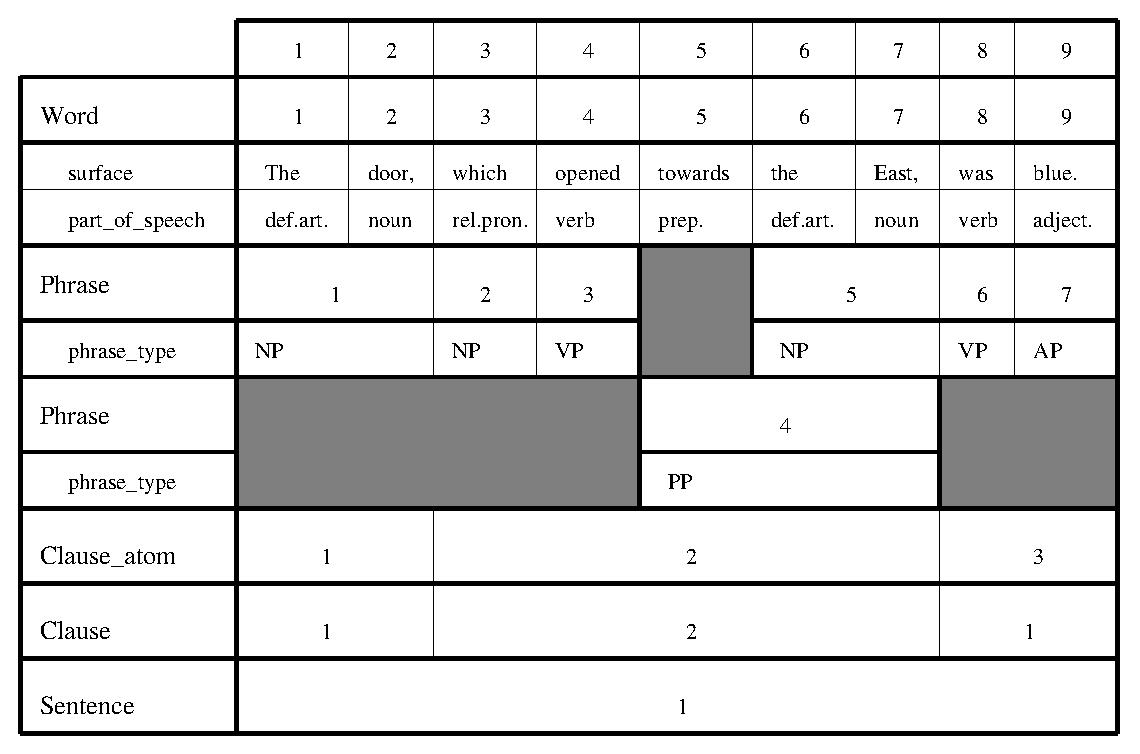
\includegraphics[width=0.6\paperwidth,keepaspectratio]{TheDoor}
\par\end{centering}
\caption{Exemplifying the four major concepts of the EMdF model:
monad, object, object type, and feature.}

\label{TheDoor}
\end{figure}
At the top of the figure, you see the sequence of monads, 1 to 9.
Just below this sequence, you see the object type ``Word'' with
its object ordinals, 1 to 9. In this example, the granularity is ``one
monad, one word.'' Thus \emph{Word} number 1 corresponds to \emph{monad}
number 1, but they are really separate entities. Word number 1 \emph{consists
of} the set of monads \{1\}. 

This becomes clearer when you notice that Clause number 2 consists
of the set of monads \{3,4,5,6,7\}. Thus there is a fundamental distinction
between the number of an object (also called object ordinal), and
the set of monads making up that object.

Some of the object types in the figure (Word and Phrase) have a number
of \emph{features}. The object type ``Word'' has the features ``surface''
and ``part\_of\_speech''. The ``Phrase'' object type has only
one feature, namely ``phrase\_type''.

Notice that objects can be discontiguous. The Clause object with object
ordinal 1 consists of the monads \{1,2,8,9\}. Thus there can be gaps
in an object.

Notice also that an object type need not have features. The object
types Clause\_atom, Clause, and Sentence have no features in the figure.

\section{Other concepts}

\subsection{Introduction}

Having learned the basic concepts of the EMdF model,
we now turn to the additional concepts which we use to talk about
EMdF databases. These concepts are:
\begin{enumerate}
\item The special object types pow\_m, any\_m,
and all\_m
\item object ids (id\_d, id\_m)
\item self
\item part\_of
\item gaps
\item borders, first, and last
\item enumerations
\item min\_m and max\_m
\item arbitrary monad sets
\item databases
\end{enumerate}

\subsection{pow\_m}

In each EMdF database, we assume an abstract
object type, pow\_m. This object type has one object for every possible
set of monads. Thus the pow\_m object type has objects consisting
of the sets \{1\},\{2\},\{3\}, \ldots , \{1,2\}, \{1,3\}, \{1,4\},
\ldots , \{2,3\},\{2,4\},\{2,5\},\ldots ,\{1,2,3\},\{1,2,4\}, \ldots ,
etc. Every possible set of monads is represented in the pow\_m object
type.

The pow\_m object type is an \emph{abstract} object
type. That is, no objects of type pow\_m actually
exist in the EMdF database. However, it is useful
to be able to talk about a particular pow\_m object. In effect, a
pow\_m object is simply a set of monads, and sometimes,
it is convenient to be able to talk about a particular pow\_m
object. This is especially true with gaps (see below).

The pow\_m object type has no features.

\subsection{any\_m}

The any\_m object type is an abstract object type like pow\_m. Each
of its objects consist of a single monad. So the any\_m objects are:
\{1\}, \{2\}, \{3\}, \ldots{} etc. The any\_m object type has no features.

\subsection{all\_m\label{subsec:all_m}}

The all\_m object type has only one object, and it consists of all
the monads in the database. That is, it consists of the monads from
min\_m to max\_m (see sections
\vref{SELECT_MIN_M} and \vref{SELECT_MAX_M}), the smallest and the
largest monads in use in the database at any given time. This one
object is called all\_m-1.

\subsection{object ids (id\_d, id\_m)}

Each object in the database (apart from pow\_m
objects) has an \emph{object id\_d}. An object id\_d is a unique ID
assigned to the object when the object is created. The id\_d is used
only for that particular object, and the id\_d is never used again
when the object is deleted.

A feature can have the type ``id\_d'', meaning that the values of
the feature are taken from the id\_ds in the database.

Each object in the database (including pow\_m,
any\_m, and all\_m objects) also has an id\_m. The id\_m is simply
the set of monads which makes up the object. This is not strictly
an ID, since objects of the same object type may have exactly the
same monads. However, for historical reasons, this is called an id\_m.
See \cite{Doedens94} or \cite{Standard-MDF} for details.

\subsection{self\label{self}}

Each object type in the database (apart from the pow\_m,
any\_m, and all\_m object types) has a feature called ``self''.
This is used to get the object id\_d of the object in question. 

The ``self'' feature is a read-only feature, which means that you
cannot update an object's self feature, or write to it when creating
the object. The value of the ``self'' feature is assigned automatically
when the object is created.

The type of the ``self'' feature is ``id\_d''.

\subsection{part\_of\label{part_of}}

If all of the monads of one object, O$_{1}$, are contained within
the set of monads making up another object, O$_{2}$, we say that
O$_{1}$ is part\_of O$_{2}$.

For example, an object with the monads \{1,2\} would be part\_of another
object with the monads \{1,2,4\}.

In mathematical terms, O$_{1}$ is part\_of O$_{2}$ if and only if
O$_{1}$ $\subseteq$ O$_{2}$.

\subsection{gaps\label{gaps}}

Objects may have gaps. A gap in an object is a maximal stretch of
monads which are not part of the object, but which are nevertheless
within the boundaries of the endpoints of the object. For example,
an object consisting of the monads \{1,3,4,7,8,13\} has three gaps:
\{2\}, \{5,6\}, and \{9,10,11,12\}.

Note that gaps are always maximal, i.e., extend across the whole of
the gap in the object. For example, \{6\} is not a gap in the above
object: instead, \{5,6\} is.

\subsection{borders, first, last\label{borders, first, last}}

Each non-empty object, being a set of monads, has a left border and
a right border. The left border is the lowest monad in the set, while
the right border is the highest monad in the set. These are also called
the first monad and the last monad in the object. If we have an object
O, the notation for these monads is O.first and O.last.

For example, if we have an object O consisting of the monads \{2,3,4,5\},
then O.first = 2 and O.last = 5.

\subsection{consecutive with respect to a set of monads\label{consecutive}}

The basic idea is that two sets of monads are consecutive if they
follow each other without any gaps in between. However, this idea
is extended so that the ``no gaps in between'' is interpreted with
respect to a reference set of monads called Su. For example, if Su
= \{1,2,5,6\}, then the sets \{2\} and \{5\} are consecutive with
respect to Su. However, the sets \{2\} and \{6\} are not consecutive
with respect to Su, since there is a ``gap'' consisting of the monad
5 in between the two sets. Likewise, the sets \{1\} and \{5\} are
not consecutive with respect to Su, because Su has a monad, 2, which
is a ``gap'' between the two sets.

\subsection{enumerations}

\subsubsection{Definition}

Each feature, it will be remembered, is of a certain type. These can
be integers, strings, and id\_ds, but they can also be enumerations.
An enumeration is a set of pairs, where each pair consists of a constant-identifier
and an integer value. 

\subsubsection{Example}

For example, the enumeration ``phrase\_type\_t'' might have the
pairs of constants and values as in table \vref{phrase_type_t}.

\begin{table}[htbp]
\begin{centering}
\begin{tabular}{|l|c|}
\hline 
constant & value\\
\hline 
\hline 
phrase\_type\_unknown & -1\\
\hline 
VP & 1\\
\hline 
NP & 2\\
\hline 
AP & 3\\
\hline 
PP & 4\\
\hline 
AdvP & 5\\
\hline 
ParticleP & 6\\
\hline 
\end{tabular}
\par\end{centering}
\caption{phrase\_type\_t enumeration}

\label{phrase_type_t}
\end{table}

\subsubsection{Default constant}

Each enumeration has exactly one default constant which is used when
the user does not give a value for a feature with that enumeration
type. In this example, ``phrase\_type\_unknown'' might be the default.

\subsubsection{Terminology}

The constants are called \emph{enumeration
constants}, while the type gathering the enumeration constants into
one whole is called an \emph{enumeration}.

\subsubsection{Names are identifiers}

The names of both enumerations and enumeration constants must be
\emph{identifiers}.


\subsubsection{Each enumeration is a name-space}

Each enumeration forms its own namespace. All name-spaces in the MQL
language are orthogonal to each other. This means that two enumeration
constants within the same enumeration cannot be called by the same
constant-identifier, but two enumeration constants in two different
enumerations may be the same. For more information, see section \vref{subsec:Namespaces}
for more information.

\subsubsection{Enumeration constants must be unique}

Enumeration constants must be unique within each enumeration, both
in their values and in their names. For example, you cannot have two
labels with the same name in the same enumeration. Nor can you have
two labels with the same value in the same enumeration, even if the
labels have different names.

This is different from C or C++ enumerations, where the same value
can be assigned to different labels.

Thus an enumeration is effectively a one-to-one correspondence (also
called a bijective function) between a set of label names and a set
of values.

\subsection{min\_m, max\_m\label{min_m,max_m}}

An EMdF database has a knowledge of which is the smallest monad in use
(min\_m) and which is the largest monad in use (max\_m). Normally, you
don't need to worry about these; the database maintains its knowledge
of these monads without your intervention. You can, however, query the
database for the minimum and maximum monads (see sections
\vref{SELECT_MIN_M} and \vref{SELECT_MAX_M}), and when you query the
database for objects, this is done within the confines of the minimum
and maximum monads.  Thus it is useful to know of their existence, but
you needn't worry too much about them.

The associated statements are SELECT MIN\_M (section \vref{SELECT_MIN_M})
and SELECT MAX\_M (section \ref{SELECT_MAX_M}).

\subsection{Arbitrary monad sets\label{subsec:Arbitrary-monad-sets}}

Each database has a central repository of monad sets which are not
associated with any objects. That is, they are not objects, have no
object type, and no features. They are just plain monad sets.

These monad sets can be used as the basis for searches. That is, when
doing a SELECT ALL OBJECTS query (or SELECT FOCUS OBJECTS), one can
specify within which arbitrary monad set the search should be conducted.

The associated statements are SELECT MONAD SETS (section \vref{subsec:SELECT-MONAD-SETS}),
GET MONAD SETS (section \vref{subsec:GET-MONAD-SETS}), CREATE MONAD
SET (section \vref{CREATE-MONAD-SET}), UPDATE MONAD SET (section
\vref{UPDATE-MONAD-SET}), and DROP MONAD SET (section \vref{DROP-MONAD-SET}).

\subsection{Computed features (monad\_set\_length, monad\_count, first\_monad,
last\_monad)}

The following computed features can always be used on any object type,
even though they are never declared:
\begin{itemize}
\item first\_monad(<monad\_set\_name>)
\item last\_monad(<monad\_set\_name>)
\item monad\_count(<monad\_set\_name>)
\item monad\_set\_length(<monad\_set\_name>)
\end{itemize}
The ``<monad\_set\_name>'' inside the parentheses must be a valid
monad set name, such as the name of a feature of type ``SET OF MONADS'',
or the privileged monad set feature, ``monads''.

If the <monad\_set\_name> to be used is the privileged ``monads''
monad set feature, the parenteses and the name ``monads'' can be
omitted, as a short-cut.

The features mean the folllowing:
\begin{description}
\item [{first\_monad(<monad\_set\_name>):}] Retrieve the <monad\_set\_name>
monad set, and yield its smallest (first) monad. For example, the
monad set ``\{1-3\}'' has first\_monad = 1.
\item [{last\_monad(<monad\_set\_name>):}] Retrieve the <monad\_set\_name>
monad set, and yield its largest (last) monad. For example, the monad
set ``\{1-3\}'' has first\_monad = 3.
\item [{monad\_count(<monad\_set\_name>):}] Retrieve the <monad\_set\_name>
monad set, and yields the number of monads in it, i.e., its cardinality.
For example, the monad set ``\{1-3, 5\}'' has a monad\_count of
4, since it has 4 monads in it (``1, 2, 3, 5''). Also, the monad
set ``\{3\}'' has a monad\_count of 1, while the monad set ``\{2-4\}''
has a monad\_count of 3 (``2, 3, 4'').
\item [{monad\_set\_length(<monad\_set\_name>):}] Retrieve the <monad\_set\_name>
feature, and yield the number \\
\\
last\_monad(<monad\_set\_name>) - first\_monad(<monad\_set\_name>)
+ 1\\
\\
For example, the set ``\{1-3, 5\}'' has a monad\_set\_length of
5 - 1 + 1 = 5. \\
Note that if the monad set has no gaps, then this will be the same
as monad\_count(<monad\_set\_name>). If, on the other hand, the monad
set has gaps, the monad\_set\_length(<monad\_set\_name>) will be strictly
greater than monad\_count(<monad\_set\_name>). 
\end{description}

\subsection{Databases}

The EMdF model has a concept of ``database.'' It is an organizational
concept which generally corresponds to what the back-end database
system calls a ``database.'' Within a database, there is one string
of monads starting at 1 and extending upwards to some very large number.
Within this stretch of monads, the user is free to create objects.

You may need to issue the USE DATABASE statement as the first thing
you do before doing anything else, in order to tell Emdros which
database you want to deal with. Ask the implementor of your Emdros
application whether this is what you should do.

A database can be created with the CREATE DATABASE statement.

\section{Encryption\label{sec:Encryption}}

Dr. D. Richard Hipp, the author of SQLite, makes an encryption-enabled
version available for a fee. There is skeleton support for SQLite
encryption in Emdros, meaning one should be able to use Dr. Hipp's
encryption-enabled version of SQLite with Emdros and get encryption-support
in Emdros on SQLite. This has not been tested, however; only the skeleton
is there. See <http://www.hwaci.com>, the website of Dr. Hipp's consulting
company, for more information about Dr. Hipp's encryption.

In this manual, when we speak of ``encryption'' on SQLite, please
be aware that the actual encryption is not a part of Emdros, and you
will achieve the exact same results and generate the exact same Emdros
databases whether you use a key or not, unless you obtain an encryption-enabled
SQLite from somewhere.

\chapter{MQL database manipulation\label{chapter:MQL Query Language}}

\section{Preliminaries}

\subsection{Introduction}

In this section on preliminaries, we will talk about four things.
First, we describe what terminals are used in the grammar-fragments
in this manual. Second, we describe the lexical conventions of MQL.
Third, we describe the name-spaces available in MQL. And finally,
we describe some top-level constraints in MQL syntax.

\subsection{Terminals}

The following terminals are used in this grammar:
\begin{itemize}
\item T\_IDENTIFIER 
\item T\_INTEGER
\item T\_STRING
\item T\_MARKS
\item \texttt{``strings''}, e.g., \texttt{``OBJECT''.}
\end{itemize}
The fifth kind, e.g., \texttt{``OBJECT''} represent keywords in
MQL. They are parsed as case-insensitive strings without the quotes. 

\subsection{Lexical conventions\label{subsec:Lexical-conventions}}

The lexical conventions for MQL are as follows:
\begin{enumerate}
\item There are two kinds of comments:

\begin{enumerate}
\item Enclosed in ``/{*}'' (opening) and ``{*}/'' (closing). This kind
of comment can span multiple lines. This is the same as C-style comments. 
\item Starting with ``//'' and ending at the end of the line. This is
the style used in C++.
\end{enumerate}
\item All keywords (such as \texttt{``CREATE''}, \texttt{``SELECT''},
\texttt{``<=''}, etc.) are case-\emph{in}sensitive insofar as they
are made up of letters. Keywords are enclosed in \texttt{``double
quotes''} in the syntax-sections below.
\item A T\_IDENTIFIER
begins with any letter (a-z,A-Z) or an underscore (\_), followed by
zero or more letters (a-z,A-Z), numbers (0-9), or underscores (\_).
For example, ``Word'', ``\_delimiter'', ``i18n'', and ``phrase\_type\_t''
are all identifiers. However, ``8bf'' is not an identifier because
it does not start with a letter or an underscore. Neither is bf@foo.com
an identifier, because it does not consist solely of letters, underscores,
and numbers.

Whether a T\_IDENTIFIER is case-sensitive
depends on what it stands for (i.e., what its ``referent'' is).
See table \ref{cap:Case-sensitivity-of-T_IDENTIFIERs} for a description.
\item A T\_INTEGER is any sequence of one
or more digits (0-9). For example, ``0'', ``42'', and ``747''
are all integers.
\item A T\_STRING is one of two kinds:

\begin{enumerate}
\item A T\_STRING can start with a single quote ('), followed by zero or
more characters which are not single quotes, and ending with another
single quote ('). Such a string can contain newlines.
\item A T\_STRING can also start with a double quote (\textquotedbl ),
followed by zero or more characters, escape-sequences (see table \ref{Escape-sequences}),
or newlines, and ending with a double quote (\textquotedbl ).
\end{enumerate}
\item \label{T_MARKS-definition}A T\_MARKS
is a sequence of one or more identifiers, each prefixed by a backping
(`). For example, the following are all T\_MARKS: ```yellow'', ```red`context'',
```marks`are`useful'', ```Flash\_Gordon`was`a`Hero''. More precisely,
a T\_MARKS conforms to the regular expression \textquotedbl (`{[}a-zA-Z\_{]}{[}a-zA-Z\_0-9{]}{*})+\textquotedbl .
\item White-space (spaces, newlines, and tabs) is ignored except in T\_STRINGs.
\end{enumerate}

\begin{table}
\begin{centering}
\begin{tabular}{|l|l|}
\hline 
T\_IDENTIFIER referent & Case-sensitivity\\
\hline 
\hline 
Database name & insensitive\\
\hline 
Object type name & insensitive\\
\hline 
Enumeration name & insensitive\\
\hline 
Enumeration constant name & sensitive\\
\hline 
\end{tabular}
\par\end{centering}
\caption{Case-sensitivity of T\_IDENTIFIERs\label{cap:Case-sensitivity-of-T_IDENTIFIERs}}
\end{table}

\begin{table}[htbp]
\begin{centering}
\begin{tabular}{|c|l|}
\hline 
Escape sequences & Meaning\\
\hline 
\hline 
\textbackslash n & newline (ASCII 10)\\
\hline 
\textbackslash t & horizontal tab (ASCII 9)\\
\hline 
\textbackslash v & vertical tab (ASCII 11)\\
\hline 
\textbackslash b & backspace (ASCII 8)\\
\hline 
\textbackslash a & bell (ASCII 7)\\
\hline 
\textbackslash r & carriage-return (ASCII 13)\\
\hline 
\textbackslash f & form-feed (ASCII 12)\\
\hline 
\textbackslash\textbackslash{} & slash (\textbackslash ) (ASCII 92)\\
\hline 
\textbackslash ? & question-mark (?) (ASCII 63)\\
\hline 
\textbackslash ' & single quote (') (ASCII 39)\\
\hline 
\textbackslash\textquotedbl{} & double quote (\textquotedbl ) (ASCII 34)\\
\hline 
\textbackslash ooo & Octal number (e.g., \textbackslash 377 is 255)\\
\hline 
\textbackslash xXX & Hexadecimal number (e.g., \textbackslash xFF is 255)\\
\hline 
\end{tabular}
\par\end{centering}
\caption{Escape sequences in strings enclosed in double quotes.}

\label{Escape-sequences}
\end{table}

\subsection{Name-spaces\label{subsec:Namespaces}}

A name-space, in computer-terminology, is a language-domain with fixed
borders within which names must be unique. \emph{Within} a name-space,
two different entities \emph{cannot} be called by the same name without
causing a name-clash. In other words, within a name-space, names must
be unique. However, if two name-spaces are \emph{orthogonal} to each
other, then a name from one name-space \emph{can} be the same as a
name from the other name-space \emph{without} causing a name-clash.

In MQL, the following name-spaces exist. They are all orthogonal to
each other:
\begin{itemize}
\item Each object type forms a name-space with respect to its features.
That is, a single object type cannot have two features with the same
name, but different object types can have features with the same name.
The two features with the same name need not even have the same feature
type. This is because all name-spaces are orthogonal to each other.
\item Each enumeration forms a name-space
with respect to its constants. That is,
a single enumeration cannot have two enumeration constants with the
same name, but different enumerations can have enumeration constants
with the same name. Since all name-spaces are orthogonal to each other,
the two enumeration constants with the same name need not have the
same integer value.
\item Each database forms a global name-space with respect to object type
names. That is, object type names must be globally unique within a
database. However, since all name-spaces are orthogonal to each other,
you can have features or enumeration constants which have the same
name as an object type.
\end{itemize}

\subsection{Top-level constraints on MQL syntax}

The MQL engine can receive any number (greater than or equal to 1)
of MQL statements. The only requirement is that each statement must
end with the keyword \texttt{``GO''}. This keyword acts as a delimiter
between each statement. The last statement may also be terminated
with \texttt{``GO''}, but need not be. Single statements on their
own need not be terminated with \texttt{``GO''} either.

If you connect to the MQL engine in daemon-mode, you must append the
meta-level statement ``QUIT'' after the ``GO'' of
the last statement.

\section{Return types}

\subsection{Introduction}

MQL is made up of statements, each of which either returns something
or doesn't. If it returns something, there are two possibilities for
what the return-type can be. It can be:
\begin{enumerate}
\item A table, or
\item A sheaf 
\end{enumerate}

\subsection{Output-formats}

The MQL engine gives you three options for using the results of an
MQL query:
\begin{enumerate}
\item You can specify that you want XML output.
\item You can specify that you want output for displaying on a console.
\item You can use the datatype provided if your program is in the same process
as the mql library.
\end{enumerate}
If you use the mql(1) program for output, please
see the manual page for how to choose the output kind.

\subsection{Tables\label{Return_types:Tables}}

The tables will look differently, depending on whether you choose
XML-output or console-output.
In the descriptions below, we will give abstract schemas for the tables,
such as the following:

\begin{tabular}{|c|c|c|}
\hline 
object\_type\_name : string & monad : monad\_m & id\_d : id\_d\\
\hline 
\end{tabular}
This means that, in each row in the table, the first piece of data
will be a string (called object\_type\_name), the second piece of
data will be a monad\_m (called monad), and the last piece of data
will be an id\_d (called id\_d). And then the row stops. There will
always be the same number of columns in each row.

A table of values may be empty, meaning it has no rows. In this case,
there will still be a table heading with type-specifications.

Some MQL statements do not return a value. In this case, there will
be no result, not even an empty table.

\subsection{Atomic output-types in tables}

The following types can get into a table and will be announced in
the header of the table:
\begin{enumerate}
\item string
\item integer
\item boolean (true or false)
\item id\_d
\end{enumerate}

\subsection{Other return values}

A number of other values are also returned from each query:
\begin{enumerate}
\item A boolean indicating whether there were any compiler-errors.
\item A boolean indicating whether there were any database-errors.
\item An integer showing which stage of the compilation/interpretation we
had come to when we exited the function (see table \vref{Table:Compiler-stages}).
In XML, this is a string as
shown in the table, of the attribute ``stage'' attribute of the
``error\_stage'' element.
\item A string carrying any error messages.
\end{enumerate}
\begin{table}[htbp]
\begin{centering}
\begin{tabular}{|l|c|l|}
\hline 
Stage & Value & XML string\\
\hline 
\hline 
None & 0 & none\\
\hline 
Parsing & 1 & parse\\
\hline 
Weeding & 2 & weed\\
\hline 
Symbol-checking & 3 & symbol\\
\hline 
Type-checking & 4 & type\\
\hline 
Monads-checking & 5 & monads\\
\hline 
Execution & 6 & exec\\
\hline 
\end{tabular}
\par\end{centering}
\caption{Compiler stages\label{Table:Compiler-stages}. \protect \\
See include/mql\_execution\_environment.h for ready-made \#define
macros.}
\end{table}

\section{Database manipulation}

\subsection{CREATE DATABASE\label{CREATE_DATABASE}}

\subsubsection{Syntax}

\begin{lyxcode}
create\_database\_statement~:~``CREATE''~~``DATABASE''

~~~~database\_name~opt\_WITH\_KEY~opt\_USING\_ENCODING

;

database\_name~:~T\_IDENTIFIER

~~~~~~~~~~~~~~|~T\_STRING

;

opt\_WITH\_KEY~:~/{*}~Empty:~No~key~is~used.~{*}/

~~~~~~~~~~~~~|~``WITH''~~``KEY''~~T\_STRING

;

opt\_USING\_ENCODING~:~/{*}~Empty:~Default~encoding~is~used.~{*}/

~~~~~~~~~~~~~~~~~~|~``USING''~~``ENCODING''~~T\_STRING

;
\end{lyxcode}

\subsubsection{Example}

\begin{lyxcode}
CREATE~DATABASE~book\_test

GO

CREATE~DATABASE~book\_test\_utf8~

USING~ENCODING~'utf-8'

GO

CREATE~DATABASE~book\_test\_latin1

USING~ENCODING~'iso-8859-1'

GO
\end{lyxcode}

\subsubsection{Explanation}

The CREATE DATABASE statement creates and initializes a database.
No text data is put into the database, and no object types are created,
but the structures necessary for the EMdF engine to function are set
in place. The user need not worry about these structures. Interested
users are referred to \cite{Rel-EMdF}.

You must CREATE a database before you can USE it (see section \ref{USE DATABASE}).
Alternatively, if you have a database that is already created but
not initialized, you can use the INITIALIZE DATABASE statememt (see
Section \vref{INITIALIZE_DATABASE}).

If a transaction was in progress (see BEGIN TRANSACTION statement,
section \vref{subsec:BEGIN-TRANSACTION}), the transaction is automatically
committed before the CREATE DATABASE statement is executed. Thus the
user need not, cannot, and should not commit it or abort it.

The database name can be either a T\_IDENTIFIER
or a T\_STRING. For MySQL and PostgreSQL,
it must be a T\_IDENTIFIER. For SQLite, it can be a T\_STRING giving
the filename (optionally including the full path) of the file in which
the database is to be created. If no path is given, the file is created
in the current working directory.

The optional ``WITH KEY'' syntax can be used on SQLite to send a
key to SQLite's sqlite\_open\_encrypted API when opening the database.
Note that this will not actually perform any encryption at all unless
you obtain an encryption-enabled SQLite from somewhere, e.g., Dr.
Hipp himself, the author of SQLite. See Section \vref{sec:Encryption}
for more information.

The optional ``WITH ENCODING'' syntax can be used to specify the
default encoding to be used for the database when creating it in the
backend database. Currently, the following values are supported:
\begin{itemize}
\item \textquotedbl utf-8\textquotedbl{}
\item \textquotedbl iso-8859-1\textquotedbl{}
\end{itemize}
If the WITH ENCODING clause is not supplied, then the default encoding
is used. The default encoding for each database is given in the following
list:
\begin{itemize}
\item PostgreSQL: iso-8859-1
\item MySQL: iso-8859-1
\item SQLite 2: iso-8859-1
\item SQLite 3: utf-8
\end{itemize}
For SQLite 3, the only encoding available is \textquotedbl utf-8\textquotedbl .
To specify any other encoding would be an error.

Note that the encoding specified only has a bearing on how the database
backend interprets the data, not on how Emdros interprets the data.
In fact, Emdros most likely will not interpret the data at all, but
rather will pass whatever is stored in the database on to the application
using Emdros, which must the interpret the data according to domain-specific
knowledge of which encoding has been used.

\subsubsection{Return type}

There is no return value.

\subsection{INITIALIZE DATABASE\label{INITIALIZE_DATABASE}}

\subsubsection{Syntax}

\begin{lyxcode}
initialize\_database\_statement~:~``INITIALIZE''~~``DATABASE''

~~~~database\_name~opt\_WITH\_KEY

;

database\_name~:~T\_IDENTIFIER

~~~~~~~~~~~~~~|~T\_STRING

;

opt\_WITH\_KEY~:~/{*}~Empty:~No~key~is~used.~{*}/

~~~~~~~~~~~~~|~``WITH''~~``KEY''~~T\_STRING

;
\end{lyxcode}

\subsubsection{Example}

\begin{lyxcode}
INITIALIZE~DATABASE~book\_test

GO
\end{lyxcode}

\subsubsection{Explanation}

The INITIALIZE DATABASE statement initializes a database without creating
it first. That is, the database must exist before issuing this statement.
It simple creates all the meta-data necessary for having an Emdros
database. This is useful on MySQL and PostgreSQL if you don't have
privileges to create databases, but you do have privileges to create
tables in an already-provided database. On SQLite, it is also useful,
if you want to add Emdros information to an already-existing SQLite
database. Other than not creating the database, this statement accomplishes
the same things as the CREATE DATABASE statement (see Section \vref{CREATE_DATABASE}).

For the optional ``WITH KEY'' syntax, please see the CREATE DATABASE
statement.

There is no ``WITH ENCODING'' syntax for the INITIALIZE DATABASE
statement. This is because the encoding is only used when CREATEing
the database. However, the internal metadata of the database is set
to the default given under the explanation for CREATE DATABASE (see
Section \vref{CREATE_DATABASE}).

\subsubsection{Return type}

There is no return value.

\subsection{USE DATABASE\label{USE DATABASE}}

\subsubsection{Syntax}

\begin{lyxcode}
use\_database\_statement~:~``USE''~~{[}~``DATABASE''~{]}~

~~~~database\_name~~opt\_WITH\_KEY

;

database\_name~:~T\_IDENTIFIER

~~~~~~~~~~~~~~|~T\_STRING

;

opt\_WITH\_KEY~:~/{*}~Empty:~No~key~is~used.~{*}/

~~~~~~~~~~~~~|~``WITH''~~``KEY''~~T\_STRING

;
\end{lyxcode}

\subsubsection{Example}

\begin{lyxcode}
USE~book\_test

GO
\end{lyxcode}
This is equivalent to
\begin{lyxcode}
USE~DATABASE~book\_test

GO
\end{lyxcode}
On SQLite:
\begin{lyxcode}
USE~DATABASE~\textquotedbl c:\textbackslash\textbackslash EmdrosDBs\textbackslash\textbackslash mydb.db\textquotedbl ~/{*}~On~SQLite~you~can~do~this.~{*}/

GO
\end{lyxcode}
With a key:
\begin{lyxcode}
/{*}~On~SQLite~you~can~get~encryption~{*}{*}{*}{*}IF{*}{*}{*}{*}~you~have~an~

~~~encryption-enabled~SQLite.~{*}/

USE~DATABASE~\textquotedbl c:\textbackslash\textbackslash Emdros\textbackslash\textbackslash MySecretDB.db\textquotedbl ~

/{*}~The~format~and~length~of~the~key~depends~on~your~SQLite

~~~encryption~implementation.~This~is~just~an~example.~{*}/

WITH~KEY~\textquotedbl\textbackslash x45\textbackslash x98\textbackslash xbf\textbackslash x12\textbackslash xfa\textbackslash xc6\textquotedbl ~

GO
\end{lyxcode}

\subsubsection{Explanation}

Before you can start using a database you have CREATEd (see section
\vref{CREATE_DATABASE}) or INITIALIZEd (see section \vref{INITIALIZE_DATABASE}),
you must connect to it using the USE DATABASE statement. The keyword
``DATABASE'' is optional and can be left out.

If a transaction was in progress (see BEGIN TRANSACTION statement,
section \vref{subsec:BEGIN-TRANSACTION}), the transaction is automatically
committed before the USE DATABASE statement is executed. Thus the
user need not, cannot, and should not commit it or abort it.

The database name can be either a T\_IDENTIFIER
or a T\_STRING. For MySQL and PostgreSQL,
it must be a T\_IDENTIFIER. For SQLite, it can be a T\_STRING giving
the filename (optionally including the full path) of the file holding
the database to be used. If no path is given, the file must be in
the current working directory.

\subsubsection{Return type}

There is no return value.

\subsection{DROP DATABASE}

\subsubsection{Syntax}

\begin{lyxcode}
drop\_database\_statement~:~``DROP''~``DATABASE''

~~~~database\_name

;

database\_name~:~T\_IDENTIFIER

~~~~~~~~~~~~~~|~T\_STRING

;
\end{lyxcode}

\subsubsection{Example}

\begin{lyxcode}
DROP~DATABASE~book\_test

GO
\end{lyxcode}

\subsubsection{Explanation}

A previously CREATEd database (see section \ref{CREATE_DATABASE})
can be completely removed from the system using this statement. All
data in the database is irretrievably lost, including all objects,
all object types, and all enumerations.

If a transaction was in progress (see BEGIN TRANSACTION statement,
section \vref{subsec:BEGIN-TRANSACTION}), the transaction is automatically
committed before the DROP DATABASE statement is executed. Thus the
user need not, cannot, and should not commit it or abort it.

The database name can be either a T\_IDENTIFIER
or a T\_STRING. For MySQL and PostgreSQL,
it must be a T\_IDENTIFIER. For SQLite, it can be a T\_STRING giving
the filename (optionally including the full path) of the file holding
the database to be dropped. If no path is given, the file must be
in the current working directory.

\subsubsection{Return type}

There is no return value.

\subsection{VACUUM DATABASE}

\subsubsection{Syntax}

\begin{lyxcode}
vacuum\_database\_statement~:~``VACUUM''~{[}~``DATABASE''~{]}

~~~~~~~~~~~~~~~~~~~~~~~~~~~~{[}~``ANALYZE''~{]}

;
\end{lyxcode}

\subsubsection{Example}

\begin{lyxcode}
1.~VACUUM~DATABASE

~~~GO~\\
~\\
2.~VACUUM~DATABASE~ANALYZE

~~~GO
\end{lyxcode}

\subsubsection{Explanation}

On PostgreSQL, this statement vacuums the database using the ``VACUUM''
SQL statement. If the optional keyword ``ANALYZE'' is given, the
statement issues a ``VACUUM ANALYZE'' statement. See the PostgreSQL
documentation for what this does.

On MySQL, this statement issues OPTIMIZE TABLE queries for all object
types. If the ANALYZE keyword is given, ANALYZE TABLE queries are
issued as well.

On SQLite, this statement first deletes all redundant sequence info
(compacting the sequence tables), then issues a VACUUM statement to
SQLite.

The significance of this statement to Emdros development is that,
when populating a database, things will speed up dramatically if the
database is VACUUM'ed after every 1000 objects created, or so.

\subsubsection{Return type}

There is no return value.

\subsection{DROP INDEXES\label{DROP-INDEXES}}

\subsubsection{Syntax}

\begin{lyxcode}
drop\_indexes\_statement~:~``DROP''~``INDEXES''

~~~~~~~~~~~~~~~~~~~~~~~~~``ON''~``OBJECT''~(``TYPE''~|~``TYPES'')

~~~~~~~~~~~~~~~~~~~~~~~~~``{[}''~object\_type\_to\_drop\_indexes\_on~``{]}''

;

object\_type\_to\_drop\_indexes\_on~:~object\_type\_name~|~``ALL''

;

object\_type\_name~:~T\_IDENTIFIER

;
\end{lyxcode}

\subsubsection{Example}

\begin{lyxcode}
1.~DROP~INDEXES

~~~ON~OBJECT~TYPES

~~~{[}ALL{]}

~~~GO~\\
~\\
2.~DROP~INDEXES

~~~ON~OBJECT~TYPE

~~~{[}Word{]}

~~~GO
\end{lyxcode}

\subsubsection{Explanation}

Emdros creates indexes on the tables associated with object types
when they are created. These indexes speed up retrieval, but slow
down insertion. Therefore, if you are going to insert a large amount
of objects, it is best to drop indexes on the object types you are
going to modify (possible all object types), then create the indexes
again after you have inserted all objects.

This statement drop indexes that have previously been create. It has
no effect if the indexes have been dropped already. If ``ALL'' is
specified as the object type, then all object types in the current
database will have their indexes dropped (if not dropped already).

The manage\_indices program that comes with the Emdros distribution
can be used to achieve the same effect.

Note that the choice between ``TYPE'' and ``TYPES'' is just syntactic
sugar. It doesn't matter which you use.

If a feature has been declared WITH INDEX, this index is dropped.
However, the feature will have its index recreated upon a CREATE INDEXES
statement affecting that object type.

\subsubsection{Return type}

There is no return value.

\subsection{CREATE INDEXES\label{CREATE-INDEXES}}

\subsubsection{Syntax}

\begin{lyxcode}
create\_indexes\_statement~:~``CREATE''~``INDEXES''

~~~~~~~~~~~~~~~~~~~~~~~~~``ON''~``OBJECT''~(``TYPE''~|~``TYPES'')

~~~~~~~~~~~~~~~~~~~~~~~~~``{[}''~object\_type\_to\_create\_indexes\_on~``{]}''

;

object\_type\_to\_create\_indexes\_on~:~object\_type\_name~|~``ALL''

;

object\_type\_name~:~T\_IDENTIFIER

;
\end{lyxcode}

\subsubsection{Example}

\begin{lyxcode}
1.~CREATE~INDEXES

~~~ON~OBJECT~TYPES

~~~{[}ALL{]}

~~~GO~\\
~\\
2.~CREATE~INDEXES

~~~ON~OBJECT~TYPE

~~~{[}Word{]}

~~~GO
\end{lyxcode}

\subsubsection{Explanation}

Emdros creates indexes on the tables associated with object types
when they are created. These indexes speed up retrieval, but slow
down insertion. Therefore, if you are going to insert a large amount
of objects, it is best to drop indexes on the object types you are
going to modify (possible all object types), then create the indexes
again after you have inserted all objects.

This statement creates indexes that have previously been dropped.
It has no effect if the indexes are there already. If ``ALL'' is
specified as the object type, then all object types in the current
database will have their indexes created (if not there already).

The manage\_indices program that comes with the Emdros distribution
can be used to achieve the same effect.

Note that the choice between ``TYPE'' and ``TYPES'' is just syntactic
sugar. It doesn't matter which you use.

\subsubsection{Return type}

There is no return value.

\section{Transactions}

\subsection{BEGIN TRANSACTION\label{subsec:BEGIN-TRANSACTION}}

\subsubsection{Syntax}

\begin{lyxcode}
begin\_transaction\_statement~:~``BEGIN''~~``TRANSACTION''

;
\end{lyxcode}

\subsubsection{Example}

\begin{lyxcode}
BEGIN~TRANSACTION

GO
\end{lyxcode}

\subsubsection{Explanation}

On PostgreSQL, this statement begins a transaction if no transaction
is in progress already. The return value is a boolean saying whether
the transaction was started (true) or not (false). If this value is
false, the user should not subsequently issue a COMMIT TRANSACTION
or ABORT TRANSACTION statement. If this value is true, the user should
issue either a COMMIT TRANSACTION or an ABORT TRANSACTION later.

On MySQL, this has no effect, and always returns false.

On SQLite, the behavior is the same as on PostgreSQL.

The transaction, if started, is automatically committed if a CREATE
DATABASE, USE DATABASE, DROP DATABASE or QUIT statement
is issued before a COMMIT TRANSACTION or ABORT TRANSACTION statement
has been issued.

Also, the transaction is automatically committed if the connection
to the database is lost, e.g., if the mql(1) program reaches the end
of the MQL stream (e.g., an MQL script) and thus has to close down.
Transactions are not maintained across invocations of the mql(1) program.
The transaction is also committed if the EMdFDB, CMQL\_execution\_environment,
or CEmdrosEnv object is destroyed.

\subsubsection{Return type}

A table with the following schema: 

\begin{tabular}{|c|}
\hline 
transaction\_started : boolean\\
\hline 
\end{tabular}
This table is empty if and only if there was a compiler error, i.e.,
if the syntax was not obeyed. The statement cannot fail with a database
error. If no transaction was started, false is returned. If a transaction
was started, true is returned.

\subsection{COMMIT TRANSACTION\label{COMMIT-TRANSACTION}}

\subsubsection{Syntax}

\begin{lyxcode}
commit\_transaction\_statement~:~``COMMIT''~~``TRANSACTION''

;
\end{lyxcode}

\subsubsection{Example}

\begin{lyxcode}
COMMIT~TRANSACTION

GO
\end{lyxcode}

\subsubsection{Explanation}

Commits the current transaction, if one is in progress. Has no effect
if a transaction was not in progress. In such cases, false is returned.

If the commit failed, false is returned. If the commit succeeded,
true is returned.

NOTE that this is slightly different from other statements which flag
a DB error if unsuccessful. Here, no DB error is flagged, but false
is returned in the table.

\subsubsection{Return type}

A table with the following schema: 

\begin{tabular}{|c|}
\hline 
transaction\_committed : boolean\\
\hline 
\end{tabular}
This table is empty if and only if there was a compiler error, i.e.,
if the syntax was not obeyed. The statement cannot fail with a database
error. If no transaction was started when the COMMIT TRANSACTION statement
was invocated, false is returned. If a transaction was started, and
it was committed successfully, true is returned. If a transaction
was started, but it was not committed successfully, false is returned.

\subsection{ABORT TRANSACTION\label{ABORT-TRANSACTION}}

\subsubsection{Syntax}

\begin{lyxcode}
abort\_transaction\_statement~:~``ABORT''~~``TRANSACTION''

;
\end{lyxcode}

\subsubsection{Example}

\begin{lyxcode}
ABORT~TRANSACTION

GO
\end{lyxcode}

\subsubsection{Explanation}

Aborts the current transaction, if one is in progress. Has no effect
if a transaction was not in progress. In such cases, false is returned.

If the abort failed, false is returned. If the abort succeeded, true
is returned.

NOTE that this is slightly different from other statements which flag
a DB error if unsuccessful. Here, no DB error is flagged, but false
is returned in the table.

\subsubsection{Return type}

A table with the following schema: 

\begin{tabular}{|c|}
\hline 
transaction\_aborted : boolean\\
\hline 
\end{tabular}
This table is empty if and only if there was a compiler error, i.e.,
if the syntax was not obeyed. The statement cannot fail with a database
error. If no transaction was started when the ABORT TRANSACTION statement
was invocated, false is returned. If a transaction was started, and
it was aborted successfully, true is returned. If a transaction was
started, but it was not aborted successfully, false is returned.

\section{Object type manipulation}

\subsection{CREATE OBJECT TYPE\label{CREATE_OBJECT_TYPE}}

\subsubsection{Syntax}

\begin{lyxcode}
create\_object\_type\_statement~:~``CREATE''~

~~~~{[}~``OBJECT''~{]}~``TYPE''

~~~~opt\_if\_not\_exists

~~~~opt\_range\_type

~~~~opt\_monad\_uniqueness\_type

~~~~``{[}''~~object\_type\_name~~~

~~~~~~~~~~~{[}~feature\_declaration\_list~{]}

~~~~``{]}''

;

opt\_if\_not\_exists:

~~~/{*}~empty:~Throw~an~error~if~object~type~exists~already~{*}/

~~|~``IF''~~``NOT''~~``EXISTS''

;

opt\_range\_type:

~~~~/{*}~empty:~Same~as~WITH~MULTIPLE~RANGE~OBJECTS~{*}/

~~|~``WITH''~~``SINGLE''~~``MONAD''~~``OBJECTS''

~~|~``WITH''~~``SINGLE''~~``RANGE''~~``OBJECTS''

~~|~``WITH''~~``MULTIPLE''~``RANGE''~~``OBJECTS''

;

opt\_monad\_uniqueness\_type~:

~~~~/{*}~empty:~same~as~WITHOUT~UNIQUE~MONADS~{*}/

~~|~``HAVING''~~``UNIQUE''~~``FIRST''~~``MONADS''

~~|~``HAVING''~~``UNIQUE''~~``FIRST''~~``AND''~~``LAST''~~``MONADS''

~~|~``WITHOUT''~~``UNIQUE''~~~``MONADS''

;

object\_type\_name~:~T\_IDENTIFIER

;

feature\_declaration\_list~:~feature\_declaration~~

~~~~\{~feature\_declaration~\}

;

feature\_declaration~:~~feature\_name~~``:''~~feature\_type~

~~~~{[}~default\_specification~{]}~~~``;''

~~~~|~feature\_name~``:''~list\_feature\_type~``;''

;

feature\_type~:~

~~~~~~~``INTEGER''~~{[}with\_index\_specification{]}

~~~~|~~``ID\_D''~~~~~{[}with\_index\_specification{]}

~~~~|~``STRING''~~~~{[}from\_set\_specification{]}~~{[}with\_index\_specification{]}~

~~~~|~``ASCII''~~~~~{[}from\_set\_specification{]}~~{[}with\_index\_specification{]}

~~~~|~set\_of\_monads\_specification

~~~~|~T\_IDENTIFIER~/{*}~For~enumerations.~{*}/

;

list\_feature\_type~:

~~~~~~``LIST''~~``OF''~~``INTEGER''~~

~~~~|~``LIST''~~``OF''~~``ID\_D''~~

~~~~|~``LIST''~~``OF''~~T\_IDENTIFIER~~/{*}~For~enumerations~{*}/

;

with\_index\_specification~:~~

~~~~|~``WITH''~~``INDEX''

~~~~|~``WITHOUT''~~``INDEX''

;

from\_set\_specification~:~``FROM''~~``SET''

;

set\_of\_monads\_specification~:~

~~~~|~``SINGLE''~``MONAD''~``SET''~``OF''~``MONADS''

~~~~|~``SINGLE''~``RANGE''~``SET''~``OF''~``MONADS''

~~~~|~``MULTIPLE''~``RANGE''~``SET''~``OF''~``MONADS''

~~~~|~``SET''~``OF''~``MONADS''~/{*}~Same~as~MULTIPLE~RANGE~SET~OF~MONADS~{*}/

;

default\_specification~:~``DEFAULT''~expression~

;

expression~:~signed\_integer~/{*}~integer~and~id\_d~{*}/

~~~~|~T\_STRING

~~~~|~T\_IDENTIFIER~/{*}~enumeration~constant~{*}/

~~~~|~monad\_set

;

signed\_integer~:~T\_INTEGER

~~~~|~``-''~T\_INTEGER

~~~~|~``NIL''

;
\end{lyxcode}

\subsubsection{Examples}

\begin{lyxcode}
CREATE~OBJECT~WITH

WITH~SINGLE~MONAD~OBJECTS

{[}Word

~~surface:~STRING~WITHOUT~INDEX;

~~lemma~:~STRING~WITH~INDEX;

~~parsing\_tag~:~STRING~FROM~SET~WITH~INDEX;

~~psp~:~part\_of\_speech\_t;

~~parents~:~LIST~OF~id\_d;

{]}

GO

CREATE~OBJECT~TYPE

IF~NOT~EXISTS

{[}Clause

~~~parent~:~id\_d;

~~~clause\_type~:~clause\_type\_t~default~NC;

~~~functions~:~LIST~OF~clause\_function\_t;~//~An~enumeration

~~~descendants~:~LIST~OF~ID\_D;

~~~parallel\_monads~:~SET~OF~MONADS;

{]}

GO
\end{lyxcode}
The latter creates an object type called ``Clause'' with four features:
parent (Immediate Constituent of), whose type is id\_d, and clause\_type,
which has the enumeration-type clause\_type\_t and the default value
NC (which must be an enumeration constant in the clause\_type\_t enumeration).
In addition, the two features ``functions'' and ``descendants''
are created, both of which are lists. ``functions'' is a list of
enumeration constants drawn from the enumeration clause\_function\_t,
whereas the ``descendants'' feature is a list of id\_ds, which should
then point to the descendants in the tree. In addition, if the object
type ``Clause'' exists already, no error is thrown, and the object
type is left untouched.

\subsubsection{Explanation}

This statement \emph{creates an object type} in the meta-data repository
of the current database. It starts out with the keywords ``CREATE
OBJECT TYPE'', followed by an optional clause which states whether
the objects will be single-range or multiple-range (see below). After
that comes a specification of the object type name and its features
enclosed in square brackets. The \texttt{feature\_declaration\_list}
is optional, so it is possible for an object type to have no features.\footnote{Strictly, this is not true, since all object types (except pow\_m,
any\_m, and all\_m) have at
least one feature, namely the one called ``self''.
Please see section \vref{self} for more information.} 

Each feature\_declaration consists of a feature name, followed by
a colon, followed by a feature type, followed by an optional specification
of the default value.

An INTEGER, ID\_D, STRING, or ASCII feature can be declared ``WITH
INDEX''. This will put an index on the feature's column. The default
is not to add an index. This index will be dropped if a DROP INDEXES
statement is issued for the object type (see Section \vref{DROP-INDEXES}),
but it will be recreated if a CREATE INDEXES statement is issued for
the object type (see Section \vref{CREATE-INDEXES}). If a feature
is an enumeration, it is usually not a good idea to create an index
on the feature. This is because enumeration constants are usually
few in number, and it is generally not a good idea to index columns
that draw their values from a small pool of values, since this can
lead to speed decreases (O(NlogN) instead of O(N)). Therefore, the
MQL language does not allow creating indexes on enumeration features.
You can add them yourself, of course, if you like, with the backend's
corresponding SQL interface.

A STRING or ASCII feature can be declared ``FROM SET''. The default
is for it not to be from a set. This does \emph{not} mean that the
value of the feature \emph{is} a set, but rather that the values are
drawn FROM a set. Whenever an object is created or updated, and a
feature is assigned which is declared ``FROM SET'', the string value
is first looked up in a special table that maps strings to unique
integers. Then this unique integer is used in lieu of the string in
the feature column. If the string does not exist in the separate table,
it is added, with a unique integer to go with it, and that integer
is used. If the string is there, then the integer already associated
with the string is used. This gives a space savings (on MySQL and
PostgreSQL), and sometimes also a speed advantage, especially if used
on the string features of a Word object type which do no have high
cardinality (number of unique instances), and the words number many
millions. SQLite and SQLite 3 may not see any speed or space savings
advantage. Note that using FROM SET on a string may actually impede
performance (especially database loading times), especially on MySQL,
if the cardinality of the string data is high. This will likely be
the case for strings like ``surface'' and ``lemma'', which generally
should not be declared FROM SET. However, features like ``part\_of\_speech'',
``case'', ``number'', ``gender'', which all most likely have
low cardinality, might be good candidates for using a STRING FROM
SET. Thus STRING FROM SET is a performance-enhanced way of using general
strings instead of enumerations, and should be just as fast as enumerations
for most queries, provided it is not used with high-cardinality data.

The specification of the default value \texttt{(default\_specification})
consists of the keyword ``DEFAULT'', followed by an expression.
An expression is either a \texttt{signed\_integer}, a string, or an
identifier. The identifier must be an enumeration constant
belonging to the enumeration which is also the
type of the feature. The \texttt{signed\_integer} is either a signed
integer (positive or negative), or the keyword ``NIL'', meaning
the id\_d that points to no object. 

The feature ``self'' is implicitly created.
It is an error if it is declared. The ``self'' feature is a computed
feature which holds the unique object id\_d
of the object. See also \vref{self}.

The difference between ``ASCII'' and ``STRING'' is that the user
promises only to store 7-bit data in an ASCII string, whereas a STRING
string may contain 8-bit data.\footnote{ASCII strings are stored exactly the same way as 8-bit STRINGs. This
distinction is mostly obsolete.} 

In previous versions, you could specify a string length in parentheses
after the STRING or ASCII keyword. As of version 1.2.0, all strings
can have arbitrary length, with no maximum.\footnote{This is true for PostgreSQL (it is a TEXT). For MySQL, the maximum
is 4294967295 (2\textasciicircum 32 - 1) characters (it is a LONGTEXT).
On SQLite, it is a TEXT, but it is unknown how much this can hold.} The old syntax is still available, but is ignored.

If a feature is declared as a LIST OF \emph{something}, that something
has to be either INTEGER, ID\_D, or an enumeration
constant. Lists of strings are not supported. Also, you cannot declare
a default value for a list -- the default value is always the empty
list.

This statement can be ``hedged'' with the ``IF NOT EXISTS'' clause.
If this clause is included, the statement does not throw an error
if the object type exists already. Instead, the object type is left
as it is (no changes are made to what is in the database already),
and the statement returns success. If the ``IF NOT EXISTS'' clause
is omitted, the statement throws an error if the object type exists
already.

An object type can be declared ``WITH SINGLE MONAD OBJECTS'', ``WITH
SINGLE RANGE OBJECTS'' or ``WITH MULTIPLE RANGE OBJECTS''. The
difference is that:
\begin{itemize}
\item An object type which has been declared ``WITH SINGLE MONAD OBJECTS''
can only hold objects which consist of a single monad (i.e., the first
monad is the same as the last monad).
\item An object type which has been declared ``WITH SINGLE RANGE OBJECTS''
can only hold objects which consist of a \emph{single monad range},
i.e., there are no gaps in the monad set, but it consists of a single
contiguous stretch of monads (possibly only 1 monad long).
\item An object type which has been declared ``WITH MULTIPLE RANGE OBJECTS''
(the default) can hold objects which have arbitrary monad sets. 
\end{itemize}
A single-monad object must consist of only 1 monad, e.g., \{1\}, \{2\},
\{3\}. A single-range object can consist of a single monad (e.g.,
\{ 1 \}, \{ 2 \}, \{ 3 \}, etc.), or it can consist of a single interval
(e.g., \{ 6-7 \}, \{ 9-13 \}, \{ 100-121 \}, etc.). However, as soon
as an object type needs to hold objects which can consist of more
than one range (e.g., \{ 6-7, 9-13 \}), then it must be declared WITH
MULTIPLE RANGE OBJECTS. If neither is specified, then WITH MULTIPLE
RANGE OBJECTS is assumed.

There is a speed advantage of using WITH SINGLE MONAD OBJECTS over
WITH SINGLE RANGE OBJECTS, and again a speed advantage of using WITH
SINGLE RANGE OBJECTS over WITH MULTIPLE RANGE OBJECTS. The latter
is the slowest, but is also the most flexible in terms of monad sets.

In addition, and orthogonally to the range type, an object type can
be declared ``HAVING UNIQUE FIRST MONADS'', ``HAVING UNIQUE FIRST
AND LAST MONADS'', or ``WITHOUT UNIQUE MONADS''. The difference
is:
\begin{itemize}
\item An object type which has been declared ``HAVING UNIQUE FIRST MONADS''
can only hold objects which are unique in their first monad within
the object type. That is, within this object type, no two objects
may start at the same monad.
\item An object type which has been declared ``HAVING UNIQUE FIRST AND
LAST MONADS'' can only hold objects which are unique in their first
monad and in their last monad (as a pair: You are allowed to have
two objects with the same starting monad but different ending monads,
or vice versa). That is, no two objects within this object type start
at the same monad while also ending at the same monad. Note that for
object types declared WITH SINGLE MONAD OBJECTS, a ``HAVING UNIQUE
FIRST AND LAST MONADS'' restriction is upgraded to a ``HAVING UNIQUE
FIRST MONADS'' restriction, since they are equivalent for this range
type.
\item An object type which has been declared ``WITHOUT UNIQUE MONADS''
(or which omits any of the ``monad uniqueness constraints'') has
no restrictions on the monads, other than those implied by the range
type.
\end{itemize}

\subsubsection{Return type}

There is no return value.

\subsection{UPDATE OBJECT TYPE\label{UPDATE_OBJECT_TYPE}}

\subsubsection{Syntax}

\begin{lyxcode}
update\_object\_type\_statement~:~``UPDATE''~~~

~~~~{[}~``OBJECT''~{]}~~~``TYPE''

~~~~``{[}''~object\_type\_name

~~~~~~~~~~feature\_update\_list

~~~~``{]}''

;

object\_type\_name~:~T\_IDENTIFIER

;

feature\_update\_list~:~feature\_update~~~\{~feature\_update~\}

;

feature\_update~:~{[}~``ADD''~{]}~~feature\_declaration

~~~~|~``REMOVE''~~~feature\_name~~~``;''

;

feature\_name~:~T\_IDENTIFIER

;

\end{lyxcode}

\subsubsection{Example}

\begin{lyxcode}
UPDATE~OBJECT~TYPE

{[}Word

~~~~ADD~no\_of\_morphemes~:~integer;

~~~~REMOVE~surface\_without\_accents;

{]}

GO
\end{lyxcode}
This example ADDs the feature no\_of\_morphemes (being an integer),
and REMOVEs the feature surface\_without\_accents.

\subsubsection{Explanation}

This statement \emph{updates an object type}. It can either add a
feature or remove an already-existing feature. When adding a new feature,
the ADD keyword is optional. Other than that, it has exactly the same
notation as for feature declarations under the CREATE OBJECT TYPE
statement.

Removing a feature requires the REMOVE keyword, the feature name,
and a semicolon.

Both additions and removals must be terminated with semicolon, even
if the \texttt{feature\_update} is the only \texttt{feature\_update}
in the list of \texttt{feature\_update}s.

Note that the statement does not allow for \emph{changing} the type
of an already existing feature, only for adding or removing features.

\subsubsection{Return type}

There is no return value.

\subsection{DROP OBJECT TYPE}

\subsubsection{Syntax}

\begin{lyxcode}
drop\_object\_type\_statement~:~``DROP''

~~~~{[}~``OBJECT''~{]}~~~``TYPE''

~~~~``{[}``~~~object\_type\_name~~~``{]}''

;

object\_type\_name~:~T\_IDENTIFIER

;
\end{lyxcode}

\subsubsection{Example}

\begin{lyxcode}
DROP~OBJECT~TYPE

{[}Sploinks{]}

GO
\end{lyxcode}
This example drops the object type ``Sploinks'' from the database.

\subsubsection{Explanation}

This statement drops an object type entirely from the database. This
deletes not only the object type, but also all the objects of that
object type, as well as the object type's features. Enumerations which
are used as a feature type are not dropped, however.

\subsubsection{Return type}

There is no return value.

\section{Enumeration manipulation}

\subsection{CREATE ENUMERATION\label{CREATE_ENUMERATION}}

\subsubsection{Syntax}

\begin{lyxcode}
create\_enumeration\_statement~:~``CREATE''~~~

~~~~(``ENUM''~|~``ENUMERATION'')~

~~~~enumeration\_name~~~``=''~

~~~~``\{''~~ec\_declaration\_list~~``\}''

;

enumeration\_name~:~T\_IDENTIFIER

;

ec\_declaration\_list~:~ec\_declaration~~~~\{~``,''~~~ec\_declaration~\}

;

ec\_declaration~:~{[}~``DEFAULT''~{]}~~~

~~~~~~~~~~~~~~~~~ec\_name~~~

~~~~~~~~~~~~~~~~~{[}~ec\_initialization~{]}

;

ec\_name~:~T\_IDENTIFIER

;

ec\_initialization~:~``=''~signed\_integer

;

\end{lyxcode}

\subsubsection{Example}

\begin{lyxcode}
CREATE~ENUMERATION

phrase\_type\_t~=~\{~VP~=~1,~NP,~AP,~

~~~PP,~default~NotApplicable~=~-1~\}

GO
\end{lyxcode}
This particular statement creates an enumeration called ``phrase\_type\_t''
with the following constants and values:
\begin{tabular}{|l|c|c|}
\hline 
Name & Value & Default\\
\hline 
\hline 
NotApplicable & -1 & Yes\\
\hline 
VP & 1 & No\\
\hline 
NP & 2 & No\\
\hline 
AP & 3 & No\\
\hline 
PP & 4 & No\\
\hline 
\end{tabular}

\subsubsection{Explanation}

This statement creates a new enumeration and populates it with enumeration
constants.

If there is no declaration that has the ``default'' keyword, then
the first one in the list becomes the default.

If the first declaration does not have an initialization, its value
becomes 1. This is different from C and C++ \texttt{enum}s, which
get 0 as the first value by default.

If a declaration does not have an initialization, its values becomes
that of the previous declaration, plus 1. This mimics C and C++ \texttt{enum}s.

Label names must be unique within the enumeration. That is, you cannot
have two constants with the same name in the same enumeration.

Values must also be unique within the enumeration. That is, you cannot
have two different labels with the same value in the same enumeration.
This is different from C/C++ \texttt{enum}s, where two labels may
have the same value.

\subsubsection{Return type}

There is no return value.

\subsection{UPDATE ENUMERATION}

\subsubsection{Syntax}

\begin{lyxcode}
update\_enumeration\_statement~:~``UPDATE''

~~~~(``ENUM''~|~``ENUMERATION'')

~~~~enumeration\_name~~~``=''

~~~~``\{''~~~ec\_update\_list~~~``\}''

;

enumeration\_name~:~T\_IDENTIFIER

;

ec\_update\_list~:~ec\_update~~~\{~``,''~~~ec\_update~\}

;

ec\_update~:~{[}~``ADD''~{]}~{[}~``DEFAULT''~{]}

~~~~ec\_name~ec\_initialization~

~~|~``UPDATE''~~~~{[}~``DEFAULT''~{]}~~~ec\_name~~~ec\_initialization~

~~|~``REMOVE''~ec\_name~

;

ec\_name~:~T\_IDENTIFIER

;

ec\_initialization~:~``=''~signed\_integer

;

\end{lyxcode}

\subsubsection{Example}

\begin{lyxcode}
UPDATE~ENUMERATION

phrase\_type\_t~=~\{

~~~~ADD~default~Unknown~=~-99,

~~~~REMOVE~NotApplicable,

~~~~UPDATE~PP~=~5,

~~~~AdvP~=~4

\}

GO
\end{lyxcode}
This alters the table made in the example in section \ref{CREATE_ENUMERATION}
to be like this:
\begin{tabular}{|l|c|c|}
\hline 
Name & Value & Default\\
\hline 
\hline 
Unknown & -99 & Yes\\
\hline 
VP & 1 & No\\
\hline 
NP & 2 & No\\
\hline 
AP & 3 & No\\
\hline 
AdvP & 4 & No\\
\hline 
PP & 5 & No\\
\hline 
\end{tabular}

\subsubsection{Explanation}

This statement updates the enumeration
constants of an already existing enumeration. The user can specify
whether to add, remove, or update an enumeration constant.

It is an error (and none of the updates will be executed) if the user
REMOVEs the default enumeration constant
without specifying a new default.

Note that you are forced to specify values for all of the constants
updated or added. 

It is an error (and none of the updates will be executed) if the update
would lave the enumeration in a state where two labels would have
the same value. This is because an enumeration is effectively a one-to-one
correspondence between a set of labels and a set of values.

It is the user's responsibility that the update leaves the database
in a consistent state. For
example, Emdros will not complain if you remove a constant with a
given value without specifying a different constant with the same
value, even if there are features that use this enumeration and have
this value. This would mean that those feature-values could not be
searched for, since there would be no label to look for.
Neither would it be possible to get the feature values with GET FEATURES,
since there would be no label to return.

\subsubsection{Return type}

There is no return value.

\subsection{DROP ENUMERATION}

\subsubsection{Syntax}

\begin{lyxcode}
drop\_enumeration\_statement~:~``DROP''~

~~~~(``ENUM''~|~``ENUMERATION'')

~~~~enumeration\_name

;

enumeration\_name~:~T\_IDENTIFIER

;
\end{lyxcode}

\subsubsection{Example}

\begin{lyxcode}
DROP~ENUMERATION~phrase\_type\_t

GO
\end{lyxcode}

\subsubsection{Explanation}

This statement removes an enumeration altogether from the database,
including all its enumeration constants.

It is an error (and impossible) to drop an enumeration which is in
use by some object type.

\subsubsection{Return type}

There is no return value.

\section{Segment manipulation}

\subsection{Introduction}

Segments were present in Emdros up to and including version 1.1.12.
After that, support for segments was removed. 

A segment used to be an arbitrary, contiguous stretch of monads which
was given a name. Objects could not be created which crossed the boundaries
of a segment. You could restrict your search to within a single segment
with SELECT ALL OBJECTS.

However, segments were found to be ugly baggage, cumbersome and not
useful. Therefore, they were removed.

The CREATE SEGMENT statement is retained for backward compatibility.

\subsection{CREATE SEGMENT\label{CREATE_SEGMENT}}

\subsubsection{Syntax}

\begin{lyxcode}
create\_segment\_statement~:~``CREATE''~~~``SEGMENT''

~~~~segment\_name

~~~~``RANGE''~~~``=''~~~segment\_range

;

segment\_name~:~T\_IDENTIFIER

;

segment\_range~:~T\_INTEGER~``-''~T\_INTEGER

;

\end{lyxcode}

\subsubsection{Example}

\begin{lyxcode}
CREATE~SEGMENT~Old\_Testament

RANGE~=~1~-~500000

GO
\end{lyxcode}
This example used to create a segment named ``Old\_Testament'' starting
at monad 1 and ending at monad 500000. 

Now it does nothing.

\subsubsection{Explanation}

This statement currently does nothing. It will fail with a database
error.

\subsubsection{Return type}

There is no return value.

\section{Querying the data}

This section describes statements which can be used to query the \emph{data}
in an Emdros database, as opposed to querying the \emph{schema}.

\subsection{SELECT (FOCUS|ALL) OBJECTS\label{SELECT_OBJECTS}}

\subsubsection{Syntax}

\begin{lyxcode}
select\_objects\_statement~:~select\_clause~

~~~~opt\_in\_clause

~~~~opt\_with\_max\_range\_clause

~~~~opt\_returning\_clause

~~~~where\_clause

;

/{*}

~{*}~select-clause

~{*}/

select\_clause~:~``SELECT''~~~focus\_specification~~~{[}~``OBJECTS''~{]}

;

focus\_specification~:~``FOCUS''~|~``ALL''

;

/{*}

~{*}~in-clause

~{*}/

opt\_in\_clause~:~``IN''~~~in\_specification

~~|~/{*}~empty~=~all\_m-1~{*}/

;

in\_specification~:~monad\_set~

~~|~``ALL''~/{*}~=~all\_m-1~{*}/

~~|~monad\_set~

~~|~T\_IDENTIFIER~/{*}~Named~arbitrary~monad~set~{*}/

;

monad\_set~:~``\{''~~~monad\_set\_element\_list~~~``\}''

;

monad\_set\_element\_list~:~monad\_set\_element~~~

~~~~\{~``,''~~~monad\_set\_element~\}

;

monad\_set\_element~:~T\_INTEGER

~~|~T\_INTEGER~~~``-''~~~T\_INTEGER

~~|~T\_INTEGER~~~``-''~~~/{*}~From~T\_INTEGER~to~``practical~infinity''

~~~~~~~~~~~~~~~~~~~~~~~~~~~(i.e.,~MAX\_MONAD).~{*}/

;

~

/{*}

~{*}opt\_with\_max\_range\_clause

~{*}/

opt\_with\_max\_range\_clause~:~``WITH''~``MAX''~``RANGE''~``MAX\_M''~``MONADS''

~~~|~/{*}~empty;~same~as~WITH~MAX~RANGE~MAX\_M~MONADS.~{*}/

~~~|~``WITH''~``MAX''~``RANGE''~T\_INTEGER~``MONADS''

~~~|~``WITH''~``MAX''~``RANGE''~``FEATURE''~``MONADS''~``FROM''~``{[}``~object\_type\_name~``{]}''

~~~|~``WITH''~``MAX''~``RANGE''~``FEATURE''~feature\_name~``FROM''~``{[}``~object\_type\_name~``{]}''

;

/{*}

~{*}~returning-clause

~{*}/

opt\_returning\_clause~:~/{*}~Empty:~Return~full~sheaf~{*}/

~~|~``RETURNING''~``FULL''~``SHEAF''

~~|~``RETURNING''~``FLAT''~``SHEAF''

~~|~``RETURNING''~``FLAT''~``SHEAF''~~``ON''~

~~~~object\_type\_name\_list~

;

object\_type\_name\_list~:~

~~object\_type\_name~\{~``,''~object\_type\_name~\}

;

/{*}

~{*}~where-clause

~{*}/

where\_clause~:~``WHERE''~mql\_query

;
\end{lyxcode}

\subsubsection{Example}

\begin{lyxcode}
SELECT~ALL~OBJECTS

IN~\{~1-4,~5,~7-9~\}

WITH~MAX~RANGE~5~MONADS

RETURNING~FULL~SHEAF

WHERE

{[}Word~lexeme~=~''>RY/''{]}

GO
\end{lyxcode}

\subsubsection{Explanation\label{SELECT OBJECTS: Explanation}}

This statement is a front-end to the MQL Query-subset (see chapter 4
starting on page \pageref{chapter:MQL Query Subset}).

The parameters to an MQL query are:
\begin{enumerate}
\item A universe U,
\item A substrate Su, and
\item A topograph.
\end{enumerate}
The universe U is a contiguous stretch of monads.
The search is restricted only to include objects which are wholly
contained within this universe (i.e., which are part\_of\footnote{For part\_of, see section \vref{part_of}.}
the universe).

The substrate is used to further restrict the search.
For there is the additional requirement that all objects found must
be wholly contained within (i.e., part\_of)
the substrate as well. The substrate
must be part\_of the universe. Mathematically
speaking, the substrate is the set intersection of whatever was in
the IN clause and all\_m-1 (i.e., the set of all monads in the database).

The topograph is what is specified as \texttt{mql\_query} in the above
grammar.

The IN-specification tells the query-engine what the substrate
Su should be. There are three choices:
\begin{enumerate}
\item Specify an explicit monad set like ``\{ 1-3000, 7000-10000 \}''
\item Specify a named arbitrary monad set (see section \vref{subsec:Arbitrary-monad-sets}).
\item Leave it blank. This means that the substrate is
calculated as all\_m-1 (i.e., all of the monads
in the database; see \cite{Standard-MDF} or \cite{Doedens94} or
page \pageref{subsec:all_m} in this Programmer's Guide.)
\end{enumerate}
The universe U is then calculated as all the monads
between the first and last monads of the substrate.

The ``max range'' specifies the maximum number of monads to take
as a context for any power block at the outermost level. The significance
of this is that it helps users not to get query results which are
correct but useless because the query returns too many straws in the
sheaf. This is done by putting an upper limit on the number of monads
a power block may extend over. This limit can be ``MAX\_M'' monads,
meaning that there is in practice no limit to the stretch of monads
which can be matched by a power block. It can also be empty, which
is the same as ``MAX\_M'' monads, i.e., no limit. It can also be
an explicit number of monads, say, 5 or 100. The max range can also
be taken as the length of the largest object of any object type. The
set of monads to use can be either the privileged ``monads'' feature,
or any feature whose type is SET OF MONADS. Note that the limit is
NOT taken as the length of any actual object of the given object type
which happens to be part\_of the current stretch of monads under investigation.
Rather, the cap is set before query execution time by inspecting the
largest length of any monad set of the given monad set feature in
the object type.

The difference between the RETURNING FULL SHEAF and the RETURNING
FLAT SHEAF clause is that the latter applies the ``flatten'' operator
to the sheaf before returning it, whereas the former does not. If
the returning\_clause clause is empty, it means the same thing as
RETURNING FULL SHEAF. If the RETURNING FLAT SHEAF has an ON appendix
with a list of object type names, then the two-argument flatten operator
is applied using this list of object type names. See section \vref{subsec:Flat-sheaf}
for an explanation of flat sheaves and the ``flatten''
operator.

\subsubsection{Monad set}

The explicit monad set in the IN clause, if given, must consist of
a comma-separated list of monad-set-elements enclosed in curly braces.
A monad-set-element is either a single integer (referring to a single
monad) or a range consisting of two integers (referring to a range
of monads). The monad-set-elements need not occur in any specific
order, and are allowed to overlap. The result is calculated by adding
all the monads together into one big set. The ranges of monads must,
however, be monotonic, i.e., the second integer must be greater than
or equal to the first.

\subsubsection{Return type}

A sheaf, either full or flat: All
retrieved objects are included, but those objects that had the \texttt{focus}
modifier in the query are flagged as such. Please see \vref{sheaf}
for an explanation of the sheaf. Appendix \vref{Appendix:Console-sheaf-grammar}
gives the grammar for the console-sheaf.
Please see section \vref{subsec:Flat-sheaf} for an explanation of
the flat sheaf.

\subsection{SELECT OBJECTS AT}

\subsubsection{Syntax}

\begin{lyxcode}
select\_objects\_at\_statement~:~``SELECT''~~~{[}~``OBJECTS''~{]}

~~~~``AT''~~~single\_monad\_specification

~~~~``{[}''~~object\_type\_to\_find~~~``{]}''

;

single\_monad\_specification~:~``MONAD''~~~``=''~~~T\_INTEGER

;

object\_type\_to\_find~:~object\_type\_name

;

object\_type\_name~:~T\_IDENTIFIER

;
\end{lyxcode}

\subsubsection{Example}

\begin{lyxcode}
SELECT~OBJECTS

AT~MONAD~=~3406

{[}Clause{]}

GO
\end{lyxcode}
This example selects all those objects of type Clause which start
at monad 3406.

\subsubsection{Explanation}

This statement returns a table containing the object id\_ds of all
the objects of the given type which start at the monad specified,
i.e., whose first monad is the given monad.

The result is a table with one column, namely ``id\_d''. Each row
represents one object, where the id\_d is its object id\_d.

\subsubsection{Return type}

A table with the following schema: 

\begin{tabular}{|c|}
\hline 
id\_d: id\_d\\
\hline 
\end{tabular}
On failure, this table is empty. Note, however, that the table can
also be empty because there were no objects of the given type having
the given monad as their first monad. This is not an error.

\subsection{SELECT OBJECTS HAVING MONADS IN}

\subsubsection{Syntax}

\begin{lyxcode}
select\_objects\_having\_monads\_in\_statement~:

~~~``SELECT''~``OBJECTS''

~~~``HAVING''~``MONADS''~``IN''

~~~monad\_set

~~~``{[}''~~object\_type\_to\_find~~~``{]}''

;

object\_type\_to\_find~:~object\_type\_name~|~``ALL''

;

object\_type\_name~:~T\_IDENTIFIER

;
\end{lyxcode}

\subsubsection{Example}

\begin{lyxcode}
SELECT~OBJECTS

HAVING~MONADS~IN~\{~23-45,~68,~70,~87-93~\}

{[}Clause{]}

GO~\\
~\\
SELECT~OBJECTS

HAVING~MONADS~IN~\{~1,~5-7,~103-109~\}

{[}ALL{]}

GO~\\
~\\
SELECT~OBJECTS

HAVING~MONADS~IN~\{~23~\}

{[}Word{]}

GO

\end{lyxcode}

\subsubsection{Explanation}

This statement returns the object types and object id\_ds of the objects
that have at least one monad in the monad set specified. If ``ALL''
is specified as the object type, then this is done for all object
types in the database. If a specific object type is specified, then
that object type is used.

The returned table has one row for each object. Each object is represented
only once. The monad in each row is guaranteed to be from the set
of monads specified, and is guaranteed to be from the object in the
row.

This statement is useful in much the same way that the SELECT OBJECTS
AT statement is useful. It can be used, e.g., for getting id\_ds of
objects that must be displayed as part of the results of a query,
but which are not in the query results. This statement can also be
used like the SELECT OBJECTS AT statement by simply making the monad
set a singleton set with only one monad. Note, however, that this
statement does something a different from SELECT OBJECTS AT. Whereas
SELECT OBJECTS AT will only retrieve an object if that object \emph{starts
on }the given monad, this present statement will retrieve the object
if only the object \emph{has at least one monad }from the monad set
given. This statement also has the advantage that one can ask for
all object types. This enables one to access objects which one knows
might be there, but of which one does not know the object types. It
also has the advantage of being much faster than a series of SELECT
OBJECTS AT statements if one is looking for objects in more than one
monad.

This statement was typically used in a series of SELECT OBJECTS HAVING
MONADS IN, GET MONADS, and GET FEATURES statements, in order to obtain
all information necessary for display of data. This sequence has been
wrapped neatly into the GET OBJECTS HAVING MONADS IN statement, which
is now the preferred method of doing this sequence.

Note to programmers: If you want to get objects not from all object
types but from only a subset of all object types, the easiest thing
is to issue the required number of copies of the statement with GO
in between, varying only the object type. That way, if you are using
the mql program as a proxy for the MQL engine, you don't incur the
overhead of starting and stopping the mql program.

\subsubsection{Return type}

\begin{tabular}{|c|c|c|}
\hline 
object\_type\_name : string & monad : monad\_m & id\_d : id\_d\\
\hline 
\end{tabular}

On failure, this table is empty. Note, however, that the table can
also be empty if the command were successful, if there were no objects
that had at least one monad in the monad set specified.

\subsection{GET OBJECTS HAVING MONADS IN}

\subsubsection{Syntax}

\begin{lyxcode}
get\_objects\_having\_monads\_in\_statement~:

~~~``GET''~``OBJECTS''

~~~``HAVING''~``MONADS''~``IN''

~~~gohmi\_monad\_set

~~~using\_monad\_set\_feature

~~~``{[}''~~object\_type\_name~~~

~~~~~~~~~~{[}gohmi\_feature\_retrieval{]}

~~~``{]}''

;

gohmi\_monad\_set~:~``ALL''~/{*}~all\_m-1~on~the~``monads''~feature,

~~~~~~~~~~~~~~~~~~~~~~~~~~~regardless~of~which~monad~set~is~actually~used!~

~~~~~~~~~~~~~~~~~~~~~~~~{*}/

~~~~~~~~~~~~~~~~|~monad\_set

;

using\_monad\_set\_feature~:~/{*}~empty:~Use~the~object's~monad~set~{*}/

~~~~|~``USING''~``MONAD''~``FEATURE''~feature\_name

~~~~|~``USING''~``MONAD''~``FEATURE''~``MONADS''

;

feature\_name~:~T\_IDENTIFIER

;

gohmi\_feature\_retrieval~:~``GET''~feature\_list

~~~~~~~~~~~~~~~~~~~~~~~~|~``GET''~``ALL''

;

feature\_list~:~feature\_name~\{~``,''~feature\_name~\}{*}

;

object\_type\_name~:~T\_IDENTIFIER

;
\end{lyxcode}

\subsubsection{Example}

\begin{lyxcode}
GET~OBJECTS

HAVING~MONADS~IN~\{~23-45,~68,~70,~87-93~\}

{[}Clause{]}

GO~\\
~\\
GET~OBJECTS

HAVING~MONADS~IN~\{~1,~5-7,~103-109~\}

USING~MONAD~FEATURE~parallel\_monads

{[}Phrase~GET~phrase\_type,~function{]}

GO~\\
~\\
GET~OBJECTS

HAVING~MONADS~IN~\{~23~\}

{[}Word~GET~ALL{]}

GO

\end{lyxcode}

\subsubsection{Explanation}

This statement returns the objects of the given object type that have
at least one monad in the monad set specified. A flat sheaf is returned
with one straw containing all the objects to be retrieved.

The monad set to use is the object's monad set by default. If the
``using\_monad\_set\_feature'' variant is used, the monad sets used
are the ones stored in this feature. The feature must be a set of
monads.

This statement is useful in much the same way that the SELECT OBJECTS
AT statement is useful. It can be used, e.g., for getting id\_ds of
objects that must be displayed as part of the results of a query,
but which are not in the query results.

This is the preferred method for getting objects from the engine,
rather than a sequence of SELECT OBJECTS HAVING MONADS IN, GET MONADS,
and GET FEATURES. It is much faster than the combination of the three.

\subsubsection{Return type}

A flat sheaf is returned which contains the objects in question. See
Section \vref{subsec:Flat-sheaf} for more information.

\subsection{GET AGGREGATE FEATURES}

\subsubsection{Syntax}

\begin{lyxcode}
get\_aggregate\_features\_statement~:~``GET''~``AGGREGATE''~(``FEATURE''~|~``FEATURES'')

~~~~aggregate\_feature\_list

~~~~``FROM''~``OBJECTS''~opt\_in\_clause

~~~~``WHERE''~

~~~~``{[}``~object\_type\_name~

~~~~~~~feature\_constraints

~~~~``{]}''

;

aggregate\_feature\_list~:~aggregate\_feature~

~~~~~~~~~~~~~~~~~~~~~~~|~aggregate\_feature\_list~``,''~aggregate\_feature

;

aggregate\_feature~:~aggregate\_function~``(``~feature\_name~``)''

~~~~~~~~~~~~~~~~~~|~``COUNT''~``(``~``{*}''~``)''

~~~~~~~~~~~~~~~~~~|~``COUNT''~``(``~feature\_name~``=''~feature\_value~``)''

;

aggregate\_function~:~``MIN''~|~``MAX''~|~``SUM''

;

feature\_name~:~T\_IDENTIFIER

;

object\_type\_name~:~T\_IDENTIFIER

;
\end{lyxcode}

\subsubsection{Examples}

\begin{lyxcode}
/{*}

~{*}~Create~the~enumerations~and~object~types~of~an~

~{*}~example~database.

~{*}

~{*}/

CREATE~ENUMERATION~boolean\_t~=~\{

~~~~false~=~0,

~~~~true

\}

GO

CREATE~ENUMERATION~part\_of\_speech\_t~=~\{

~~~~Verb,

~~~~Noun,

~~~~ProperNoun,

~~~~Pronoun,

~~~~Adjective,

~~~~Adverb,

~~~~Preposition,

~~~~Conjunction,

~~~~Particle

\}

GO

CREATE~OBJECT~TYPE

WITH~SINGLE~MONAD~OBJECTS

{[}Token

~~~~has\_space\_before~:~boolean\_t;~~//~Any~space~before~the~surface?

~~~~surface~:~STRING;~~~~~~~~~~~~~~//~The~surface~itself

~~~~has\_space\_after~:~boolean\_t;~~~//~Any~space~after~the~surface?

~~~~part\_of\_speech~:~part\_of\_speech\_t;

~~~~is\_punctuation~:~boolean\_t;~~~~~//~true~iff~the~surface~is~punctuation.

{]}

GO

CREATE~OBJECT~TYPE

WITH~SINGLE~RANGE~OBJECTS

{[}Line

~~~~actant\_name~:~STRING~FROM~SET;

~~~~gender~:~gender\_t;

~~~~words\_spoken~:~INTEGER;~

~~~~line\_number\_in\_act~:~INTEGER;

{]}

GO

/{*}

~{*}~Example~1:

~{*}

~{*}~Founds~all~Token~objects~in~the~entire~database~whose~

~{*}~is\_punctuation~feature~equals~false.

~{*}

~{*}~Then~retrieve~one~aggregate~function,~namely~a~count~of~

~{*}~all~Token~objects~whose~part\_of\_speech~is~equal~to~Verb.

~{*}/

GET~AGGREGATE~FEATURES

COUNT(part\_of\_speech=Verb)

FROM~OBJECTS

WHERE

{[}Token~is\_punctuation=false{]}

GO

/{*}~

~{*}~Example~2:

~{*}

~{*}~Finds~all~Line~objects~in~the~database~(no~monad~restriction),~and

~{*}~does~three~aggregate~functions:

~{*}~-~Find~the~sum~of~all~words~spoken~by~all~actants.

~{*}~-~Find~a~count~of~all~Line~objects.~(Note~that~this,~together~with~the

~{*}~~~sum~of~all~words~spoken,~can~be~used~to~calculate~the~average

~{*}~~~number~of~words~spoken~by~any~actant.~This~has~to~be~done~outside~of~

~{*}~~~Emdros,~as~Emdros~does~not~yet~support~floating~point~return~values.)

~{*}~-~Find~a~count~of~all~Line~objects~whose~gender~feature~is~Man,~i.e.,~the

~{*}~~~number~of~Line~spoken~by~a~Man.

~{*}/

GET~AGGREGATE~FEATURES

SUM(words\_spoken),~COUNT({*}),~COUNT(gender=Man)

FROM~OBJECTS

WHERE

{[}Line{]}

GO

/{*}

~{*}~Example~3:

~{*}

~{*}~Finds~all~Line~objects~where~actant\_name~is~equal~to~\textquotedbl Hamlet\textquotedbl ~in

~{*}~the~monad~set~\{~1-12478~\}~(an~arbitrarily~chosen~example).

~{*}~Does~three~aggregate~functions:

~{*}~-~Finds~the~maximum~number~of~words~spoken~in~any~of~\textquotedbl Hamlet\textquotedbl 's~

~{*}~~~lines.

~{*}~-~Finds~the~minimum~line~number~in~any~act~(i.e.,~the~first~line

~{*}~~~in~which~\textquotedbl Hamlet\textquotedbl ~speaks.

~{*}~-~Finds~the~total~count~of~Lines~spoken~by~\textquotedbl Hamlet\textquotedbl .

~{*}/

GET~AGGREGATE~FEATURES

MAX(words\_spoken),~MIN(line\_number\_in\_act),~COUNT({*})

FROM~OBJECTS

IN~\{~1-12478~\}

WHERE

{[}Line~actant\_name=\textquotedbl Hamlet\textquotedbl{]}

GO

/{*}

~{*}~Example~4:

~{*}

~{*}~Finds~all~Line~objects~in~all~monads,

~{*}~where~actant\_name~is~equal~to~\textquotedbl Hamlet\textquotedbl ~

~{*}~OR~is~equal~to~``Ophelia''.

~{*}~Does~three~aggregate~functions:

~{*}~-~Finds~the~total~sum~of~words~spoken~by~either~Hamlet~or~Ophelia.

~{*}~-~Finds~the~count~of~all~Lines~in~which~the~actant\_name~is~``Hamlet''.

~{*}~-~Finds~the~count~of~all~Lines~in~which~the~actant\_name~is~``Ophelia''.

~{*}/

GET~AGGREGATE~FEATURES

SUM(words\_spoken),~COUNT(actant\_name=\textquotedbl Hamlet\textquotedbl ),~COUNT(actant\_name=\textquotedbl Ophelia\textquotedbl )

FROM~OBJECTS

IN~ALL

WHERE

{[}Line~actant\_name=\textquotedbl Hamlet\textquotedbl ~OR~actant\_name=\textquotedbl Ophelia\textquotedbl{]}

GO
\end{lyxcode}

\subsubsection{Explanation}

This statement returns a table giving the desired aggregate functions
over the objects specified in the WHERE clause.

In essence, five aggregate functions are available:
\begin{description}
\item [{MIN(feature\_name):}] Retrieves the minimum value of the given
feature. The feature must be of type integer. The result is also an
integer.
\item [{MAX(feature\_name):}] Retrieves the maximum value of the given
feature. The feature must be of type integer. The result is also an
integer.
\item [{SUM(feature\_name):}] Retrieves the sum of all values of the given
feature. The feature must be of type integer. The result is also an
integer.
\item [{COUNT({*}):}] Retrieves a count of all objects retrieved by the
WHERE clause. The result is an integer.
\item [{COUNT(feature\_name=feature\_value):}] Retrieves a count of all
objects retrieves, with the added restriction that the given feature
name must have the given feature value. The result is an integer.
\end{description}
The standard SQL aggregate function ``AVG'' is missing. This is
because Emdros does not (yet) support return values with type ``floating
point''. Note that the same result as AVG can be achieved by retrieving
two aggregate functions: SUM(feature\_name) and COUNT({*}), and then
doing the appropriate division outside of Emdros.

The \texttt{opt\_in\_clause} can be used to limit the monad set within
which to retrieve the objects. If omitted, it means that the entire
database is searched, without monad restriction.

The object type name given after the ``WHERE'' and ``{[}`` tokens
is also the object type on which any features in the aggregate feature
list are found. Hence, the features mentioned in the aggregate feature
list must exist on the object type.

It is possible to use an arbitrary Boolean expression after the object
type name, just as in the topographic MQL queries explained in Chapter
\pageref{chapter:MQL Query Subset}.

\subsubsection{Return type}

Upon failure, an empty table.

Upon success, a table with one row, and as many columns as there are
aggregate functions in the query. The column types are all ``integer'',
and the column names are given as ``Column1'', ``Column2'', ...,
``Column\emph{N}'', where the number given is the index (1-based)
of the aggregate functions in the input query.

\subsection{GET MONADS\label{Section:GET MONADS}}

\subsubsection{Syntax}

\begin{lyxcode}
get\_monads\_statement~:~``GET''~``MONADS''~

~~~~``FROM''~~~(``OBJECT''~|~``OBJECTS'')

~~~~``WITH''~id\_ds\_specification

~~~~``{[}''~object\_type\_name~``{]}''

;

object\_type\_name~:~T\_IDENTIFIER

;
\end{lyxcode}

\subsubsection{Example}

\begin{lyxcode}
GET~MONADS~

FROM~OBJECTS

WITH~ID\_DS~=~10342,~10344,~10383

{[}Clause{]}

GO
\end{lyxcode}

\subsubsection{Explanation\label{GET_MONADS:Explanation}}

This statement returns, for each object in the list of id\_ds, a representation
of its set of monads. The set is represented by maximal stretches
of monads. For example, if an object consists of the monads \{ 1,
2, 4, 5, 6, 9, 11, 12 \}, and its id\_d is 10342, then the following
will be in the results of the above example:
\begin{tabular}{|c|c|c|}
\hline 
object\_id\_d : id\_d & mse\_first : monad\_m & mse\_last : monad\_m\\
\hline 
10342 & 1 & 2\\
\hline 
10342 & 4 & 6\\
\hline 
10342 & 9 & 9\\
\hline 
10342 & 11 & 12\\
\hline 
\end{tabular}

The ``mse'' in ``mse\_first'' and ``mse\_last'' stands for ``Monad
Set Element.'' A monad set element consists of a starting monad and
an ending monad (always greater than or equal to the starting monad).
It represents all of the monads between the two borders,
including the borders. An mse's last monad is always
greater than or equal to its first monad.

The mses in the list are always maximal. That is, there is a gap
of at least one monad in between each of the MSEs.

In mathematical terms, suppose we have an MSE A. Then for all other
MSEs B for the same object, it is the case that either A.last + 1
< B.first or B.last < A.first - 1

The MSEs will come in no particular order.

See \cite{Monad-Sets} for more information on monad sets and the
way Emdros treats them.

It does not matter whether you write ``OBJECT'' or ``OBJECTS'':
The choice is merely syntactic sugar.

There is no limit on how many id\_ds can be specified. The algorithm
will not balk at even many thousand id\_ds, but it will, of course,
take more time to get the monads of more objects.

This statement was typically used in a series of SELECT OBJECTS HAVING
MONADS IN, GET MONADS, and GET FEATURES statements, in order to obtain
all information necessary for display of data. This sequence has been
wrapped neatly into the GET OBJECTS HAVING MONADS IN statement, which
is now the preferred method of doing this sequence.

\subsubsection{Return type}

A table with the following schema:
\begin{tabular}{|c|c|c|}
\hline 
object\_id\_d : id\_d & mse\_first : monad\_m & mse\_last : monad\_m\\
\hline 
\end{tabular}

\subsection{GET FEATURES\label{subsec:GET-FEATURES}}

\subsubsection{Syntax}

\begin{lyxcode}
get\_features\_statement~:~``GET''~~~

~~~~(``FEATURE''~|~``FEATURES'')

~~~~feature\_list

~~~~``FROM''~~~(``OBJECT''~|~``OBJECTS'')

~~~~``WITH''~id\_ds\_specification

~~~~``{[}''~~object\_type\_name~~~``{]}''

;

/{*}

~{*}~feature\_list

~{*}/

feature\_list~:~feature\_name~~~\{~``,''~~feature\_name~\}

;

feature\_name~:~T\_IDENTIFIER

;

object\_type\_name~:~T\_IDENTIFIER

;

\end{lyxcode}

\subsubsection{Example}

\begin{lyxcode}
GET~FEATURES~surface,~psp

FROM~OBJECTS~WITH~ID\_DS~=~12513,12514

{[}Word{]}

GO
\end{lyxcode}

\subsubsection{Explanation}

This statement returns a table containing feature-values of certain
objects in the database.

Note how this is different from the ``SELECT FEATURES'' command.
The ``SELECT FEATURES'' command queries an \emph{object type} for
a list of its \emph{features}. The ``GET FEATURES'' command queries
\emph{objects} for the \emph{values} of some of their features.

This statement was typically used in a series of SELECT OBJECTS HAVING
MONADS IN, GET MONADS, and GET FEATURES statements, in order to obtain
all information necessary for display of data. This sequence has been
wrapped neatly into the GET OBJECTS HAVING MONADS IN statement, which
is now the preferred method of doing this sequence.

\subsubsection{Return type}

The return type is a table with a schema containing one string for
each feature in the list of features. The order of the columns is
that in the list of features. The first column in the table contains
the object id\_d involved in the row. Thus for $n$ features, the
number of columns will be $n+1$.

The return type of each feature is the same as the type of the feature.
The exact representation depends on whether the output is console
output or XML output. For XML, see the DTD. For console output, see
the examples below. Enumeration constants are shown as the enumeration
constant label, not the integer value. 

For list features, the value is a space-surrounded, space-delimited
list of values. Integers and ID\_Ds are given as integers; enumeration
constant values as their constant names (e.g., ``first\_person''). 

\begin{tabular}{|c|c|c|c|c|c|c|}
\hline 
object\_id\_d: id\_d & surface: string & psp: enum(psp\_t) & number\_in\_corpus : integer & parent: id\_d & parents: list\_of\_id\_d & functions : list\_of\_enum(function\_t)\\
\hline 
\end{tabular}
The table contains the objects in no particular order.

\subsection{GET SET FROM FEATURE}

\subsubsection{Syntax}

\begin{lyxcode}
get\_set\_from\_feature\_statement~:~``GET''~~~``SET''

~~~~``FROM''~~~``FEATURE''

~~~~feature\_name

~~~~``{[}''~~object\_type\_name~~~``{]}''

;

feature\_name~:~T\_IDENTIFIER

;

object\_type\_name~:~T\_IDENTIFIER

;

\end{lyxcode}

\subsubsection{Example}

\begin{lyxcode}
GET~SET~

FROM~FEATURE~lexeme

{[}Word{]}

GO
\end{lyxcode}

\subsubsection{Explanation}

This statement returns a table containing the set of existing feature-values
for a feature declared FROM SET. See the CREATE OBJECT TYPE and UPDATE
OBJECT TYPE statements on page \pageref{CREATE_OBJECT_TYPE} and \pageref{UPDATE_OBJECT_TYPE}
respectively for the syntax of the FROM SET declaration.

Note how this is different from GET FEATURES: The ``GET FEATURES''
command queries \emph{objects} for the \emph{values} of some of their
features. The GET SET FROM FEATURE queries the \emph{set} of existing
values for a given feature, regardless of which objects have these
values for this feature.

\subsubsection{Return type}

The return type is a table with a schema containing one string for
each value in the set. 

\begin{tabular}{|c|}
\hline 
value: string\\
\hline 
\end{tabular}
The order of the strings in the table is undefined.

\subsection{SELECT MIN\_M\label{SELECT_MIN_M}}

\subsubsection{Syntax}

\begin{lyxcode}
select\_min\_m\_statement~:~``SELECT''~~~``MIN\_M''

;
\end{lyxcode}

\subsubsection{Example}

\begin{lyxcode}
SELECT~MIN\_M

GO
\end{lyxcode}

\subsubsection{Explanation}

Returns the minimum monad in use in the database. The table returned
has only one data row, namely the minimum monad. See section \vref{min_m,max_m}
for more information.

\subsubsection{Return type}

A table with the following schema:

\begin{tabular}{|c|}
\hline 
min\_m : monad\_m\\
\hline 
\end{tabular}
On failure, this table is empty. 

\subsection{SELECT MAX\_M\label{SELECT_MAX_M}}

\subsubsection{Syntax}

\begin{lyxcode}
select\_max\_m\_statement~:~``SELECT''~~~``MAX\_M''

;
\end{lyxcode}

\subsubsection{Example}

\begin{lyxcode}
SELECT~MAX\_M

GO
\end{lyxcode}

\subsubsection{Explanation}

Returns the maximum monad in use in the database. The table returned
has only one data row, namely the maximum monad. See section \vref{min_m,max_m}
for more information.

\subsubsection{Return type}

A table with the following schema:

\begin{tabular}{|c|}
\hline 
max\_m : monad\_m\\
\hline 
\end{tabular}
On failure, this table is empty. 

\subsection{SELECT MONAD SETS\label{subsec:SELECT-MONAD-SETS}}

\subsubsection{Syntax}

\begin{lyxcode}
select\_monad\_sets\_statement~:~``SELECT''~``MONAD''~``SETS''

;
\end{lyxcode}

\subsubsection{Example}

\begin{lyxcode}
SELECT~MONAD~SETS~GO
\end{lyxcode}

\subsubsection{Explanation}

This statement returns a table listing the names of the monad sets
stored in the database. These are the monad sets referred to in section
\vref{subsec:Arbitrary-monad-sets}.

The monad set names come in no particular order.

\subsubsection{Return type}

\begin{tabular}{|c|}
\hline 
monad\_set\_name : string\\
\hline 
\end{tabular}

\subsection{GET MONAD SETS\label{subsec:GET-MONAD-SETS}}

\subsubsection{Syntax}

\begin{lyxcode}
get\_monad\_sets\_statement~:~``GET''~``MONAD''~(``SET''~|~``SETS'')

~~~~~~~~~~~~~~~~~~~~~~~~~~monad\_sets\_specification

;

monad\_sets\_specification~:~``ALL''

~~|~monad\_set\_list

;

monad\_set\_list~:~monad\_set\_name~\{~``,''~monad\_set\_name~\}

;

monad\_set\_name~:~T\_IDENTIFIER

;
\end{lyxcode}

\subsubsection{Example}

\begin{lyxcode}
GET~MONAD~SET~My\_research\_collection

GO

GET~MONAD~SETS~Historical\_books,~Former\_prophets

GO

GET~MONAD~SETS~ALL

GO
\end{lyxcode}

\subsubsection{Explanation}

This statement returns a table listing the monads of each of the monad
sets named in the query. These monad sets are the arbitrary monad
sets described in section \vref{subsec:Arbitrary-monad-sets}.

It doesn't matter whether you say ``SET'' or ``SETS''. This is
purely syntactic sugar.

If ``ALL'' is given as the monad\_sets\_specification, then all
monad sets are listed, in no particular order.

In the output, each monad set is represented in the same way as described
in section \vref{GET_MONADS:Explanation}. Each monad set is guaranteed
to appear in the table in one contiguous stretch, that is, monad sets
are not interleaved. Moreover, the monad set elements of each monad
set is sorted on mse\_first, in ascending order.

\subsubsection{Return type}

\begin{tabular}{|c|c|c|}
\hline 
monad\_set\_name : string & mse\_first : monad\_m & mse\_last : monad\_m\\
\hline 
\end{tabular}

\section{Schema reflection}

This section describes those query statements which can be used to
retrieve information about the schema.

\subsection{SELECT OBJECT TYPES}

\subsubsection{Syntax}

\begin{lyxcode}
select\_object\_types\_statement~:~``SELECT''

~~~~{[}~``OBJECT''~{]}~~~~``TYPES''

;
\end{lyxcode}

\subsubsection{Example}

\begin{lyxcode}
SELECT~OBJECT~TYPES

GO
\end{lyxcode}

\subsubsection{Explanation}

This statement returns a list of the names of all the object types
available in the database.

\subsubsection{Return type}

A table with the following schema: 

\begin{tabular}{|c|}
\hline 
object\_type\_name: string\\
\hline 
\end{tabular}
On failure, this table is empty.

\subsection{SELECT FEATURES}

\subsubsection{Syntax}

\begin{lyxcode}
select\_features\_statement~:~``SELECT''~~~``FEATURES''

~~~~``FROM''~~~{[}~{[}~``OBJECT''~{]}~~~``TYPE''~{]}

~~~~``{[}''~~~object\_type\_name~~~``{]}''

;

object\_type\_name~:~T\_IDENTIFIER

;

\end{lyxcode}

\subsubsection{Example}

\begin{lyxcode}
SELECT~FEATURES

FROM~OBJECT~TYPE

{[}Phrase{]}

GO
\end{lyxcode}

\subsubsection{Explanation}

This statement returns a table with the features belonging to the
given object type. 

The type\_name string in the result gives the type of the feature.
It has the values as in table \ref{cap:Possible-type-names}.

The default\_value string in the result is a string representation
of the default value. It must be interpreted according to the feature
type.

The computed boolean in the result shows whether the feature is computed
or not. Currently, the only computed features
are: ``self'', ``first\_monad'', ``last\_monad'',
``monad\_count'', and ``monad\_set\_length''.

For lists, what is shown in the ``default value'' field is always
``()'' meaning ``the empty list''.

For sets of monads, a string giving the canonical form of an empty
set of monads is used: `` \{~ \} ''.

\begin{table}
\begin{centering}
\begin{tabular}{|l|l|}
\hline 
Type name & Meaning\\
\hline 
\hline 
integer & integer\\
\hline 
id\_d & id\_d\\
\hline 
list of integer & list of integer\\
\hline 
list of id\_d & list of id\_d\\
\hline 
list of \emph{something else} & list of enumeration constants from the enumeration
given\\
\hline 
string & 8-bit string of arbitrary length\\
\hline 
ascii & 7-bit (ASCII) string of arbitrary length\\
\hline 
set of monads & set of monads\\
\hline 
\emph{everything else} & enumeration by the name given\\
\hline 
\end{tabular}
\par\end{centering}
\caption{Possible type names in SELECT FEATURES\label{cap:Possible-type-names}}
\end{table}

\subsubsection{Return type}

A table with the following schema:

\begin{tabular}{|c|c|c|c|}
\hline 
feature\_name: string & type\_name: string & default\_value: string & computed: boolean\\
\hline 
\end{tabular}
On failure, this table is empty. On success, the table cannot be empty,
since every object type has the feature ``self''.

\subsection{SELECT ENUMERATIONS}

\subsubsection{Syntax}

\begin{lyxcode}
select\_enumerations\_statement~:~``SELECT''

~~~~``ENUMERATIONS''

;
\end{lyxcode}

\subsubsection{Example}

\begin{lyxcode}
SELECT~ENUMERATIONS

GO
\end{lyxcode}

\subsubsection{Explanation}

This statement returns a table with the names of all the enumerations
available in the database.

\subsubsection{Return type}

A table with the following schema: 

\begin{tabular}{|c|}
\hline 
enumeration\_name: string\\
\hline 
\end{tabular}
On failure, this table is empty. Note, however, that it can also be
empty because there are no enumerations in the database yet.

\subsection{SELECT ENUMERATION CONSTANTS}

\subsubsection{Syntax}

\begin{lyxcode}
select\_enumeration\_constants\_statement~:~``SELECT''

~~~~(``ENUM''~|~``ENUMERATION'')~~~``CONSTANTS''

~~~~``FROM''~~~~{[}~(``ENUM''~|~``ENUMERATION''~)~{]}

~~~~enumeration\_name

;

enumeration\_name~:~T\_IDENTIFIER

;

\end{lyxcode}

\subsubsection{Example}

\begin{lyxcode}
SELECT~ENUMERATION~CONSTANTS

FROM~ENUMERATION~phrase\_types

GO
\end{lyxcode}

\subsubsection{Explanation}

This statement returns a table with the enumeration
constants in a given enumeration. 

Note that the syntax is made so that the query need not be as verbose
as in the example just given. There is quite a lot of syntactic sugar\footnote{``Syntactic sugar'' is a term used by computer-scientists for niceties
in the grammar of a language which help the user in some way, usually
so that they do not have to type as much as would otherwise be required.
Here, it simply means that some of the keywords are optional, or have
shorthand forms.} in this statement.

\subsubsection{Return type}

A table with the following schema: 

\begin{tabular}{|c|c|c|}
\hline 
enum\_constant\_name: string & value : integer & is\_default : boolean\\
\hline 
\end{tabular}
On failure, this table is empty. 

\subsection{SELECT OBJECT TYPES USING ENUMERATION }

\subsubsection{Syntax}

\begin{lyxcode}
select\_object\_types\_which\_use\_enum\_statement~:~``SELECT''~

~~~~{[}~``OBJECT''~{]}~~~~``TYPES''

~~~~``USING''

~~~~(``ENUM''~|~``ENUMERATION'')~enumeration\_name

;

enumeration\_name~:~T\_IDENTIFIER

;

\end{lyxcode}

\subsubsection{Example}

\begin{lyxcode}
SELECT~OBJECT~TYPES

USING~ENUMERATION~phrase\_types\_t

GO
\end{lyxcode}

\subsubsection{Explanation}

This statement returns a table with the names of the object types
which use a given enumeration. The rows of the table are not ordered.
An object type uses an enumeration if at least one of its features
is of the enumeration type.

\subsubsection{Return type}

A table with the following schema:

\begin{tabular}{|c|}
\hline 
object\_type\_name: string\\
\hline 
\end{tabular}
On failure, this table is empty. Note, however, that it can also be
empty because there are no object types using the enumeration.

\section{Object manipulation}

\subsection{CREATE OBJECT FROM MONADS\label{CREATE_OBJECT_FROM_MONADS}}

\subsubsection{Syntax}

\begin{lyxcode}
create\_object\_from\_monads\_statement~:~``CREATE''~~~``OBJECT''

~~~~``FROM''~~~monad\_specification

~~~~{[}~with\_id\_d\_specification~{]}

~~~~object\_creation\_specification

;

/{*}

~{*}~monad-specification

~{*}/

monad\_specification~:~``MONADS''~~~``=''~~~monad\_set

;

/{*}

~{*}~with-id\_d-specification

~{*}/

with\_id\_d\_specification~:~``WITH''~~~``ID\_D''~

~~~~``=''~~id\_d\_const

;

id\_d\_const~:~T\_INTEGER

~~|~``NIL''

;

/{*}

~{*}~object-creation-specification

~{*}/

object\_creation\_specification~:~``{[}''

~~~~object\_type\_name

~~~~{[}~list\_of\_feature\_assignments~{]}

~~~~``{]}''

;

object\_type\_name~:~T\_IDENTIFIER

;

list\_of\_feature\_assignments~:~feature\_assignment~~\\
~~~~~~~~~~~~~~~~~~~~~~~~~~~~~~\{~feature\_assignment~\}

;

feature\_assignment~:~feature\_name~~``:=''~~expression~~``;''

~~~~|~feature\_name~~``:=''~~list\_expression~~``;''

;

feature\_name~:~T\_IDENTIFIER

;

expression~:~signed\_integer~/{*}~integer~and~id\_d~{*}/

~~|~T\_STRING

~~|~T\_IDENTIFIER~/{*}~enumeration~constant~{*}/

~~|~monad\_set

;

list\_expression~:~``(``~{[}list\_values{]}~``)''

;

list\_values~:~list\_value~\{~``,''~list\_value~\}

;

list\_value~:~signed\_integer

~~|~T\_IDENTIFIER~/{*}~enumeration~constant~{*}/

;

\end{lyxcode}

\subsubsection{Example}

\begin{lyxcode}
CREATE~OBJECT~FROM~MONADS~=~\{~1-2,~4-7~\}

{[}Clause

~~~clause\_type~:=~NC;

~~~parent~:=~10033;

~~~descendants~:=~(104546,~104547,~104549);

{]}

GO~\\
~\\
CREATE~OBJECTS~FROM~MONADS~=~\{~35-37~\}

WITH~ID\_D~=~104546

{[}Phrase

~~~phrase\_type~:=~NP;

~~~parents~:=~(104212,~104215,~104219);

{]}

GO
\end{lyxcode}

\subsubsection{Explanation}

This statement creates a new object from a specified set of monads.

In creating an object, four items of information are necessary:
\begin{enumerate}
\item The new id\_d,
\item The object type,
\item The set of monads, 
\item Any features that need non-default values.
\end{enumerate}
This statement creates an object of type ``\texttt{object\_type\_name}''
using the monads and features, and optional id\_d, given. All features
not specified will be given default values.

If you specify an id\_d with the ``WITH ID\_D'' specification, the
system first checks whether that object id\_d is already in use. If
it is, the creation fails. If it is not, that id\_d is used. If you
do not specify an id\_d, a unique id\_d is auto-generated.

Note that when using WITH ID\_D, it is not recommended to run several
concurrent processes against the same database which issue CREATE
OBJECT or CREATE OBJECTS statements. Doing so may cause the auto-generated
object id\_d sequence to become invalid. However, several concurrent
processes may safely issue CREATE OBJECT(S) statements if none of
them use WITH ID\_D. 

Note that objects of the special object types all\_m,
any\_m, and pow\_m cannot
be created.

\subsubsection{Return type}

A table with the following schema:

\begin{tabular}{|c|}
\hline 
object\_id\_d: id\_d\\
\hline 
\end{tabular}
On success, there is always only one row in the table, namely the
row containing the object id\_d of the newly created object.

On failure, the table is empty.

\subsection{CREATE OBJECT FROM ID\_DS\label{CREATE_OBEJCT_FROM_ID_DS}}

\subsubsection{Syntax}

\begin{lyxcode}
create\_object\_from\_id\_ds\_statement~:~``CREATE''~~~``OBJECT''

~~~~``FROM''~~~id\_ds\_specification

~~~~{[}~with\_id\_d\_specification~{]}

~~~~object\_creation\_specification

;

/{*}

~{*}~id\_ds-specification

~{*}/

id\_ds\_specification~:~(``ID\_D''~|~``ID\_DS'')~

~~~~``=''~~~id\_d\_list

;

id\_d\_list~:~id\_d~~~\{~``,''~~id\_d~\}

;

id\_d~:~id\_d\_const

;

id\_d\_const~:~T\_INTEGER

~~|~``NIL''

;

\end{lyxcode}

\subsubsection{Example}

\begin{lyxcode}
CREATE~OBJECT~FROM~ID\_DS~=~10028,~10029

{[}Clause

~~~clause\_type~:=~NC;

~~~parent~:=~10033;

{]}

GO
\end{lyxcode}

\subsubsection{Explanation}

This statement creates a new object with the monads contained in the
objects specified by their id\_ds.

The id\_ds specified are used only to calculate the set of monads
to be used. This is calculated as the union of the set of monads of
the objects with the id\_ds specified. These id\_ds can point to objects
of any type, and it need not be the same type for all id\_ds.

Note that there is a syntactic sugar-choice of whether to say ``ID\_DS''
or ``ID\_D''. 

Note that objects of the special object types all\_m,
any\_m, and pow\_m cannot
be created.

See the ``CREATE OBJECT FROM MONADS'' (section \ref{CREATE_OBJECT_FROM_MONADS}
on page \pageref{CREATE_OBJECT_FROM_MONADS}) for further explanation
and warnings. Especially about concurrent use of WITH ID\_D.

\subsubsection{Return type}

The return type is the same as for CREATE OBJECT FROM MONADS (section
\ref{CREATE_OBJECT_FROM_MONADS}). 

\subsection{CREATE OBJECTS WITH OBJECT TYPE}

\subsubsection{Syntax}

\begin{lyxcode}
create\_objects\_statement~:~``CREATE''~~``OBJECTS''

~~~~~~~~~~~~~~~~~~~~~~~~~~~``WITH''~~``OBJECT''~``TYPE''

~~~~~~~~~~~~~~~~~~~~~~~~~~~``{[}''~~object\_type\_name~~``{]}''

~~~~~~~~~~~~~~~~~~~~~~~~~~~object\_creation\_list~

;~\\
~\\
object\_creation\_list~:~object\_creation~\{~object\_creation~\}

;~\\
~\\
object\_creation~:~``CREATE''~~``OBJECT''

~~~~~~~~~~~~~~~~~~``FROM''~~monad\_specification

~~~~~~~~~~~~~~~~~~{[}~with\_id\_d\_specification~{]}

~~~~~~~~~~~~~~~~~~``{[}''~

~~~~~~~~~~~~~~~~~~{[}~list\_of\_feature\_assignments~{]}~

~~~~~~~~~~~~~~~~~~``{]}''~

;~
\end{lyxcode}

\subsubsection{Example}

\begin{lyxcode}
CREATE~OBJECTS

WITH~OBJECT~TYPE~{[}Phrase{]}

CREATE~OBJECT

FROM~MONADS~=~\{~1-2~\}

{[}~

~~phrase\_type~:=~NP;~

~~function~:=~Subj;

{]}

CREATE~OBJECT

FROM~MONADS~=~\{~3-7~\}

{[}

~~//~Use~default~values~for~phrase\_type~and~function

~~//~(probably~VP/Pred~in~this~fictive~example)

{]}~

CREATE~OBJECT

FROM~MONADS~=~\{~4-7~\}

WITH~ID\_D~=~1000000~//~Assign~specific~ID\_D

{[}

~~phrase\_type~:=~NP;

~~function~:=~Objc;

{]}

GO

\end{lyxcode}

\subsubsection{Explanation}

This statement is for batch importing of objects. It is useful when
populating databases, either from scratch or by adding large numbers
of objects to an existing database. This statement is much faster
than individual CREATE OBJECT statements.

The object type is specified only once, at the top. Note that no features
can be assigned where the object type is specified: That comes later
in the query, when each object is created.

Each object to be created must be given a monad set. The monad set
follows the syntax specified in section \vref{SELECT_OBJECTS}.

Optionally, an id\_d can be specified. If an id\_d is specified, it
is the user's responsibility to ensure that the id\_d assigned does
not clash with another id\_d in the database. This is mainly useful
when dumping/restoring databases.

If no id\_d is specified, a unique id\_d is generated. This id\_d
is only guaranteed to be unique if no other objects are created with
specific id\_ds.

Note that when using WITH ID\_D, it is not recommended to run several
concurrent processes against the same database which issue CREATE
OBJECT or CREATE OBJECTS statements. Doing so may cause the auto-generated
object id\_d sequence to become invalid. However, several concurrent
processes may safely issue CREATE OBJECT(S) statements if none of
them use WITH ID\_D.

The feature-value assignments follow the same rules as for CREATE
OBJECT FROM MONADS (see section \vref{CREATE_OBJECT_FROM_MONADS}).
If an object has a feature which is not assigned a value, the default
value is used. The default value of a given feature can be specified
when creating the object type, or when updating the object type (see
section \vref{CREATE_OBJECT_TYPE} and section \vref{UPDATE_OBJECT_TYPE}).

A table is returned showing the number of objects created successfully.
This number is valid even if the process failed half way through.
In other words, if the process did not run to completion due to a
DB error, the value in the return type will show how many objects,
if any, were created successfully. This means that there is no way
of knowing which object got which object id\_d, a difference from
the regular CREATE OBJECT statement.

\subsubsection{Return type}

A table with the following schema:

\begin{tabular}{|c|}
\hline 
object\_count: integer\\
\hline 
\end{tabular}
On both success and failure, the table contains one row showing the
number of objects created successfully.

\subsection{UPDATE OBJECTS BY MONADS\label{UPDATE_OBJECTS_BY_MONADS}}

\subsubsection{Syntax}

\begin{lyxcode}
update\_objects\_by\_monads\_statement~:~``UPDATE''~

~~~~(``OBJECT''~|~``OBJECTS'')

~~~~``BY''~~~monad\_specification~

~~~~object\_update\_specification

;

/{*}

~{*}~object-update-specification

~{*}/

object\_update\_specification~:~``{[}``~~~object\_type\_name~

~~~~list\_of\_feature\_assignments

~~~~``{]}''

;

object\_type\_name~:~T\_IDENTIFIER

;

\end{lyxcode}

\subsubsection{Example}

\begin{lyxcode}
UPDATE~OBJECTS~BY~MONADS~=~\{~1-2,~4-7,~8-20~\}

{[}Clause

~~~~clause\_type~:=~VC;

{]}

GO
\end{lyxcode}

\subsubsection{Explanation}

This statement finds all the objects of type \texttt{object\_type\_name}
which are part\_of the monads specified (i.e.,
they must be wholly contained within the monads specified), and updates
their features according to the list of feature assignments.

Note that there is a syntactic sugar-choice of whether to say ``OBJECTS''
or ``OBJECT''. This is because the user may know that only one object
is to be found within the monads, in which case having to write ``OBJECTS''
would be intellectually irritating.

Note that objects of the special object types all\_m,
any\_m, and pow\_m cannot
be updated.

The feature ``self'' cannot be updated.

\subsubsection{Return type}

A table with the following schema:

\begin{tabular}{|c|}
\hline 
object\_id\_d: id\_d\\
\hline 
\end{tabular}
On success, the table contains one row for each updated object.

On failure, the table is empty.

\subsection{UPDATE OBJECTS BY ID\_DS}

\subsubsection{Syntax}

\begin{lyxcode}
update\_objects\_by\_id\_ds\_statement~:~``UPDATE''~

~~~~(``OBJECT''~|~``OBJECTS'')

~~~~``BY''~~~id\_ds\_specification~

~~~~object\_update\_specification

;

\end{lyxcode}

\subsubsection{Example}

\begin{lyxcode}
UPDATE~OBJECTS~BY~ID\_DS~=~10028,~10029

{[}Phrase

~~~~parent~:=~10034;

{]}

GO
\end{lyxcode}

\subsubsection{Explanation}

This statement updates all the objects of the given type with the
given id\_ds.

The id\_ds should point to objects which are really of the given type.
Otherwise, an error is issued.

Note that there is a syntactic sugar-choice between ``OBJECTS''
and ``OBJECT.'' 

Note that objects of the special object types all\_m,
any\_m, and pow\_m cannot
be updated.

The feature ``self'' cannot be updated.

\subsubsection{Return type}

The return type is the same as for UPDATE OBJECTS BY MONADS (section
\vref{UPDATE_OBJECTS_BY_MONADS}).

\subsection{DELETE OBJECTS BY MONADS\label{DELETE_OBJECTS_WITH_MONADS}}

\subsubsection{Syntax}

\begin{lyxcode}
delete\_objects\_by\_monads\_statement~:~``DELETE''

~~~~(``OBJECT''~|~``OBJECTS'')

~~~~``BY''~~~monad\_specification

~~~~object\_deletion\_specification

;

/{*}

~{*}~object-deletion-specification

~{*}/

object\_deletion\_specification~:~``{[}''

~~~~object\_type\_name\_to\_delete

~~~~``{]}''

;

object\_type\_name\_to\_delete~:~object\_type\_name~

~~|~``ALL''

;

object\_type\_name~:~T\_IDENTIFIER

;

\end{lyxcode}

\subsubsection{Example}

\begin{lyxcode}
DELETE~OBJECTS~BY~MONADS~=~\{~1-20~\}

{[}Clause{]}

GO
\end{lyxcode}
If ``\texttt{object\_name\_to\_delete}'' is ``ALL'', then all
objects of all types which are at these monads are deleted:
\begin{lyxcode}
DELETE~OBJECTS~BY~MONADS~=~\{~28901-52650~\}

{[}ALL{]}

GO
\end{lyxcode}

\subsubsection{Explanation}

This command deletes all the objects of type \texttt{object\_type\_name}
which are part\_of the set of monads specified. 

\subsubsection{Return type}

A table with the following schema:

\begin{tabular}{|c|}
\hline 
object\_id\_d: id\_d\\
\hline 
\end{tabular}
On success, the table contains one row for each deleted object.

On failure, the table is empty.

\subsection{DELETE OBJECTS BY ID\_DS}

\subsubsection{Syntax}

\begin{lyxcode}
delete\_objects\_by\_id\_ds\_statement~:~``DELETE''

~~~~(``OBJECT''~|~``OBJECTS'')

~~~~``BY''~~~id\_ds\_specification

~~~~object\_deletion\_specification

;
\end{lyxcode}

\subsubsection{Example}

\begin{lyxcode}
DELETE~OBJECTS~BY~ID\_DS~10028,~10029

{[}Phrase{]}

GO
\end{lyxcode}

\subsubsection{Explanation}

This statement deletes objects by their id\_ds. Note that you cannot
write ``ALL'' for \texttt{object\_deletion\_specification}. The
id\_ds given should point to objects of the type given.

\subsubsection{Return type}

The return type is the same as for DELETE OBJECTS BY MONADS (section
\ref{DELETE_OBJECTS_WITH_MONADS}).

\section{Monad manipulation}

\subsection{MONAD SET CALCULATION\label{MONAD-SET-CALCULATION}}

\subsubsection{Syntax}

\begin{lyxcode}
monad\_set\_calculation\_statement~:~``MONAD''~~``SET''

~~~~``CALCULATION''

~~~~monad\_set\_chain

;

monad\_set\_chain~:~monad\_set~~\\
~~~~~~~~~~~~~~~~~~\{~monad\_set\_operator~~monad\_set~\}

;

monad\_set\_operator~:~``UNION''

~~|~``DIFFERENCE''

~~|~``INTERSECT''

;
\end{lyxcode}

\subsubsection{Example}

\begin{lyxcode}
//~Produces~\{~1-10~\}

MONAD~SET~CALCULATION

\{~1-5,~7-8~\}

UNION

\{~5-10~\}

GO~\\
~\\
//~Produces~\{~2-5,~22-24~\}

MONAD~SET~CALCULATION

\{~1-10,~20-30,~50-60~\}

INTERSECT

\{~2-5,~22-24~\}

GO~\\
~\\
//~Produces~\{~1-4,~8-10~\}

MONAD~SET~CALCULATION

\{~1-10~\}

DIFFERENCE

\{~5-7~\}

GO~\\
~\\
//~Produces~\{~2-3,~5-6,~10-12~\}

MONAD~SET~CALCULATION

\{~1-3,~5-9~\}

INTERSECT

\{~2-6~\}

UNION

\{~10-12~\}

GO
\end{lyxcode}

\subsubsection{Explanation}

This statement is for performing set-operations on sets of monads.
The three standard set operations ``union,'' ``intersect,'' and
``difference'' are provided.

The return value is a representation of the resulting set of monads
along the same lines as for the GET MONADS statement (see section
\ref{Section:GET MONADS}).

The MSEs (see section \ref{Section:GET MONADS}) are listed in ascending
order.

You can specify as many sets of monads as you want. The operations
are done in succession from the first to the last set of monads. For
example, in the last example above, the intersection is done first,
and the union is done on the result of the intersection.

You can also specify only one set of monads, with no set operator.
This is useful for creating a sorted, normalized set of monads from
a number of different MSEs.

Note that this statement does not manipulate the stored arbitrary
monad sets described in section \vref{subsec:Arbitrary-monad-sets}.

\subsubsection{Return type}

A table with the following schema:

\begin{tabular}{|c|c|}
\hline 
mse\_first : monad\_m & mse\_last : monad\_m\\
\hline 
\end{tabular}

\subsection{CREATE MONAD SET\label{CREATE-MONAD-SET}}

\subsubsection{Syntax}

\begin{lyxcode}
create\_monad\_set\_statement~:~``CREATE''~``MONAD''~``SET''

~~~~~~~~~~~~monad\_set\_name

~~~~~~~~~~~~``WITH''~``MONADS''~``=''~monad\_set

;

monad\_set\_name~:~T\_IDENTIFIER

;
\end{lyxcode}

\subsubsection{Example}

\begin{lyxcode}
CREATE~MONAD~SET

My\_research\_collection

WITH~MONADS~=~\{~1-10394,~14524-29342,~309240-311925~\}

GO
\end{lyxcode}

\subsubsection{Explanation}

This statement creates an arbitrary monad set in the database. These
monad sets are the ones described in section \vref{subsec:Arbitrary-monad-sets}.

\subsubsection{Return type}

There is no return value.

\subsection{UPDATE MONAD SET\label{UPDATE-MONAD-SET}}

\subsubsection{Syntax}

\begin{lyxcode}
update\_monad\_set\_statement~:~``UPDATE''~``MONAD''~``SET''

~~~~~monad\_set\_name

~~~~~(``UNION''~|~``INTERSECT''~|~``DIFFERENCE''~|~``REPLACE'')

~~~~~(monad\_set~|~monad\_set\_name)

;

monad\_set\_name~:~T\_IDENTIFIER

;
\end{lyxcode}

\subsubsection{Examples}

\begin{lyxcode}
//~Adds~the~specified~monad~set~to~``Historical\_books''

UPDATE~MONAD~SET

Historical\_books

UNION

\{~310320-329457~\}

GO

//~Remove~the~specified~monad~set~from~``Historical\_books''

UPDATE~MONAD~SET

Historical\_books

DIFFERENCE

\{~310320-329457~\}

GO

//~Intersects~the~monad~set~``My\_research\_collection''

//~with~the~monad~set~``My\_experimental\_collection''

UPDATE~MONAD~SET

My\_research\_collection

INTERSECT

My\_experimental\_collection

GO

//~Replaces~the~monad~set~``Lamentations''~with~

//~the~specified~monad~set

UPDATE~MONAD~SET

Lamentations

REPLACE

\{~380300-383840~\}

GO
\end{lyxcode}

\subsubsection{Explanation}

This statement is used to update an already-existing arbitrary monad
set (see section \vref{subsec:Arbitrary-monad-sets}). Four operations
are provided: set union, set intersection, set difference, and replacement.
In all cases, the operation is done using two monad sets. The first
set is the named set that is updated. The second set is either a set
described in terms of monads, or the name of another arbitrary monad
set.

The replacement operator effectively deletes the old set, replacing
it with the new. Note, however, that this does not imply that the
new is deleted -- if you update one named monad set, replacing it
with another named monad set, that other monad set is not deleted,
but simply copied into the old monad set.

The other three operators are standard set-theoretic operators.

\subsubsection{Return type}

There is no return value.

\subsection{DROP MONAD SET\label{DROP-MONAD-SET}}

\subsubsection{Syntax}

\begin{lyxcode}
drop\_monad\_set\_statement~:~``DROP''~``MONAD''~``SET''

~~~~~~~~~~~~~~~~~~~~~~~~~~~monad\_set\_name

;

monad\_set\_name~:~T\_IDENTIFIER

;
\end{lyxcode}

\subsubsection{Example}

\begin{lyxcode}
DROP~MONAD~SET~Historical\_books

GO
\end{lyxcode}

\subsubsection{Explanation}

This statement drops an arbitrary monad set (i.e., deletes it) from
the database. These are the arbitrary monad sets described in section
\vref{subsec:Arbitrary-monad-sets}.

\subsubsection{Return type}

There is no return value.

\section{Meta-statements}

\subsection{QUIT}

\subsubsection{Syntax}

\begin{lyxcode}
quit\_statement~:~``QUIT''

;

\end{lyxcode}

\subsubsection{Example}

\begin{lyxcode}
QUIT
\end{lyxcode}

\subsubsection{Explanation}

This causes the rest of the MQL stream not to be interpreted. It also
causes the mql(1) program to quit after having
executed this statement.

The QUIT statement can be used, e.g., if running the mql(1) program
as a daemon through xinetd(8) or inetd(8), to end the connection.

The QUIT statement is special in that it does not need a ``GO''
keyword after it. You may supply the ``GO'' keyword if you wish,
but it is not required.

If a transaction was in progress (see BEGIN TRANSACTION statement,
section \vref{subsec:BEGIN-TRANSACTION}), the transaction is automatically
committed before the QUIT statement is executed.

\subsubsection{Return type}

There is no return value.

\chapter{MQL Query subset\label{chapter:MQL Query Subset}}

\section{Introduction}

This chapter is an introduction to the query-subset of MQL for programmers.
That is, it introduces the important subset of MQL in which you can
express queries that find objects and gaps in interesting environments,
with specified interrelations, and with specified feature-values.

An easier-to-read MQL Query Guide is available from the Emdros website,
or with the Emdros sourcecode in the doc/ directory (see \cite{MQL-Query-Guide}).

First, we give an informal introduction to MQL by means of some examples
(\ref{sec:Informal-introduction-to}). Then we give a complete overview
of the syntax of the MQL query-subset (\ref{mql_query:Syntax}). Then
we explain the sheaf, which is the data-structure that an MQL query-query
returns (\ref{sheaf}). Then we explain what a Universe and a Substrate
are, since they are important in understanding how a query works (\ref{sec:Universe-and-substrate}).
After that, we explain two important properties of mql queries, namely
consecutiveness and embedding (\ref{mql-query:Consecutiveness-and-embedding}).
After that, we give detailed explanations of the blocks of the MQL
query-subset, which are the ``building blocks'' out of which a query
is made (\ref{Blocks}). Finally, we explain how strings of blocks
are written, and what they mean (\ref{sec:Strings-of-blocks}).

\section{Informal introduction to MQL by means of some examples\label{sec:Informal-introduction-to}}

\subsection{Introduction}

This section informally introduces the query-part of MQL by way of
a number of examples. The example database which we will use is the
same as in Doedens' book, namely part of
Melville's ``Moby Dick'':
\begin{quote}
``CALL me Ishmael. Some years ago - never mind how long precisely
- having little or no money in my purse, and nothing particular to
interest me on shore, I thought I would sail about a little and see
the watery part of the world. It is a way I have of driving off the
spleen, and regulating the circulation. Whenever I find myself growing
grim about the mouth; whenever it is damp, drizzly November in my
soul; whenever I find myself involuntarily pausing before coffin warehouses,
and bringing up the rear of every funeral I meet; and especially whenever
my hypos get such an upper hand of me, that it requires a strong moral
principle to prevent me from deliberately stepping into the street,
and methodically knocking people's hats off - then, I account it high
time to get to sea as soon as I can. {[}...{]}

``{[}...{]} By reason of these things, then, the whaling voyage was
welcome; the great flood-gates of the wonder-world swung open, and
in the wild conceits that swayed me to my purpose, two and two there
floated into my inmost soul, endless processions of the whale, and,
mid most of them all, one grand hoofed phantom, like a snow hill in
the air.''
\end{quote}
Suppose that we have in this EMdF database the domain-dependent object
types ``paragraph'', ``sentence'', and ``word'', which correspond
to paragraphs, sentences, and words of the text. And suppose that
we add to the object type ``sentence'' the feature ``mood,'' which
draws its values from the enumeration type \{ imperative, declarative
\}. And suppose that we add to the object type ``word'' the features
``surface'' (which gives the surface text of the word) and ``part\_of\_speech''
(which gives the part of speech of the word). The codomain of the
feature ``part\_of\_speech'' on the object type ``word'' draws
its values from the enumeration type \{ adjective, adverb, conjunction,
determiner, noun, numeral, particle, preposition, pronoun, verb \}.
This hypothetical database will give the background for most of the
examples in our informal introduction to MQL.

In the following, when we refer to an ``MQL query'', we will mean
the query-subset of MQL. That is, we abstract away from the database-manipulation-part
of MQL and concentrate on the query-queries. In addition, we will
abstract away from the required ``SELECT (FOCUS|ALL) OBJECTS'' syntax
that must precede an MQL query-query.

\subsection{topograph}

An MQL query is called a topograph. Consider the following topograph:
\begin{lyxcode}
{[}sentence{]}
\end{lyxcode}
This topograph retrieves a list of all sentence objects in the database. 

\subsection{features}

A query can specify which features an object must have for it to be
retrieved. For example, consider the following topograph:
\begin{lyxcode}
{[}word

~~~surface~=~\textquotedbl Ishmael\textquotedbl ~or~part\_of\_speech~=~verb;

{]}
\end{lyxcode}
This topograph retrieves a list of all words which either have the
surface ``Ishmael'', or whose part of speech is ``verb.''

\subsection{object\_block, object\_block\_first}

There are several types of blocks. They are meant to come in a string
of blocks, where each block in the string must match some part of
the database in order for the whole string to match. Two such blocks
are the \texttt{object\_block} and the \texttt{object\_block\_first}.

Object blocks are the heart and soul of MQL queries. They are used
to match objects and objects nested in other objects. An object block
(be it an \texttt{object\_block} or an \texttt{object\_block\_first})
consists of the following parts:
\begin{enumerate}
\item The opening square bracket, `\texttt{{[}}'.
\item An identifier indicating the object type of the objects which we wish
to match (e.g., ``phrase'').
\item An optional T\_MARKS (e.g., ```yellow''
or ```red`context''). This will be put into the result set (i.e.,
sheaf) unchanged, and can be used to pass information back into the
application from the user. The meaning of the T\_MARKS is wholly application-dependent,
since Emdros does nothing special with it --- it just passes the
T\_MARKS on into the sheaf. See page \pageref{T_MARKS-definition}
for the formal definition of T\_MARKS.
\item An optional ``object reference declaration.'' A reference to this
object can be declared with the ``\texttt{as}'' keyword, like ``\texttt{{[}word
as w} $\ldots$''. Subsequent blocks can then refer to features of
this object as ``\texttt{w}.\emph{featurename}'' (see section \vref{Object references}).
\item An optional keyword which can be either of ``\texttt{noretrieve}'',
``\texttt{retrieve}'' or ``\texttt{focus}''. The default, when
it is not specified, is ``\texttt{retrieve}''. The keyword ``\texttt{noretrieve}''
says as much as ``I do not wish to retrieve this object, even if
matched''. It is useful for specifying the context of what we really
wish to retrieve. The keyword ``\texttt{focus}'' specifies that
this object is to be retrieved (it implies ``\texttt{retrieve}''),
and also that, when sifting the sheaf for focus objects,
this object must go into the result (see section \vref{Retrieval}).
\item An optional keyword, ``\texttt{first}'' or ``\texttt{last}'',
which says as much as ``this object must be first/last in the universe
against which we are matching (see section \vref{First and last}).
\item An optional Boolean expression giving what features need to hold true
for this object for it to be retrieved (see section \vref{Feature specifications}).
This boolean expression must be prefixed by one of the words ``\texttt{feature}''
or ``\texttt{features}''. It makes no difference which is used --
it is merely syntactic sugar.
\item An optional inner \texttt{blocks} which matches objects inside the
object (see section \ref{Block strings: blocks}).
\item The closing square bracket, `\texttt{{]}}'.
\end{enumerate}
Note that only the first object block in a string of blocks can have
the ``\texttt{first}'' keyword, and only the last \texttt{object\_block}
in a string of \texttt{block}s can have the ``\texttt{last}'' keyword. 

Consider the following \texttt{topograph}:
\begin{lyxcode}
{[}sentence`yellow

~~~~mood~=~imperative;

~~~~{[}word~noretrieve~first

~~~~~~~~~surface~=~\textquotedbl CALL\textquotedbl ;

~~~~{]}

~~~~{[}word`red{]}

{]}
\end{lyxcode}
This \texttt{topograph} retrieves the set of sentences which are imperative,
and whose first word is ``CALL''. Within each sentence in that set,
we retrieve the second word, but not the first. The only sentence
in our example database which qualifies is the first sentence.

\subsection{power}

The power construct is used to indicate that we allow some distance
in between two blocks. A power construct must always stand between
two other blocks, and can thus never be first or last in a query.
It comes in three varieties: 
\begin{itemize}
\item A ``plain vanilla'' power construct, syntactically denoted by two
dots, ``\texttt{..}'', and 
\item A power construct with a single, upper limit. The limit specifies
the maximum monads that can intervene between the two surrounding
blocks. It is denoted as e.g., ``\texttt{..~<~5}'', or ``\texttt{..~<=~5}''.
\item A power construct with a compound min/max limit. The limit specifies
the minimum and maximum monads that can intervene. It is denoted as,
e.g., ``\texttt{.. BETWEEN 1 AND 5}''.
\end{itemize}
Consider the following topograph:
\begin{lyxcode}
{[}sentence

~~~~{[}word

~~~~~~~~part\_of\_speech~=~preposition{]}

~~~~..~<~4

~~~~{[}word

~~~~~~~~part\_of\_speech~=~noun{]}

~~~~..

~~~~{[}word~last

~~~~~~~~surface~=~\textquotedbl world\textquotedbl{]}

{]}
\end{lyxcode}
This topograph retrieves a list of sentences which have a word that
has part of speech preposition, followed by a word which has part
of speech noun, and which is within 4 monads of the preposition, followed
by the last word of the sentence, which must be ``world''. Within
that sentence, retrieve all the three words. The only sentence which
qualifies is the second.

\subsection{opt\_gap\_block}

An \texttt{opt\_gap\_block} is used to match an optional gap in the
text. It consists of:
\begin{enumerate}
\item The opening square bracket, `\texttt{{[}}'.
\item The keyword ``\texttt{gap?}''.
\item An optional T\_MARKS (e.g., ```yellow''
or ```red`context''). This will be put into the result set (i.e.,
sheaf) unchanged, and can be used to pass information back into the
application from the user. The meaning of the T\_MARKS is wholly application-dependent,
since Emdros does nothing special with it --- it just passes the
T\_MARKS on into the sheaf. See page \pageref{T_MARKS-definition}
for the formal definition of T\_MARKS.
\item An optional ``\texttt{noretrieve},'' ``\texttt{retrieve}'' or
``\texttt{focus}.'' The default is ``\texttt{noretrieve}''. (See
section \vref{Retrieval})
\item An optional \texttt{blocks} (see section \vref{Block strings: blocks}).
\item The closing square bracket, `\texttt{{]}}'.
\end{enumerate}
The \texttt{opt\_gap\_block} matches gaps in the \emph{substrate}
against which we are matching. Thus if we look at the example in figure
\vref{TheDoor}, we can construct the following topograph:
\begin{lyxcode}
{[}clause

~~~~{[}clause\_atom

~~~~~~~~{[}word

~~~~~~~~~~~~~surface~=~\textquotedbl door,\textquotedbl{}

~~~~~~~~{]}

~~~~{]}

~~~~{[}gap?~noretrieve{]}

~~~~{[}clause\_atom~noretrieve{]}

{]}
\end{lyxcode}
This retrieves all clauses which happen to have inside them a clause\_atom
which contains the word ``door,'', followed by a gap,
followed by a clause\_atom. The gap and the second clause\_atom
are not retrieved. This would retrieve clause-1. The gap
need not be there.

The default is for the result of an \texttt{opt\_gap\_block} not to
be retrieved. Thus one needs to explicitly write ``\texttt{retrieve}''
if one wishes to retrieve the gap.

\subsection{gap\_block}

A \texttt{gap\_block} is used to match a gap in the text.
It consists of:
\begin{enumerate}
\item The opening square bracket, `\texttt{{[}}'.
\item The keyword ``\texttt{gap}''.
\item An optional T\_MARKS (e.g., ```yellow''
or ```red`context''). This will be put into the result set (i.e.,
sheaf) unchanged, and can be used to pass information back into the
application from the user. The meaning of the T\_MARKS is wholly application-dependent,
since Emdros does nothing special with it --- it just passes the
T\_MARKS on into the sheaf. See page \pageref{T_MARKS-definition}
for the formal definition of T\_MARKS.
\item An optional ``\texttt{noretrieve},'' ``\texttt{retrieve}'' or
``\texttt{focus}.'' The default is ``\texttt{noretrieve}''. (See
section \vref{Retrieval}).
\item An optional \texttt{blocks}. (See section \vref{Block strings: blocks}).
\item The closing square bracket, `\texttt{{]}}'.
\end{enumerate}
The \texttt{gap\_block} is analogous to the \texttt{opt\_gap\_block}
in all respects except that there \emph{must} be a gap
in order for the query to match.

\subsection{object references}

An object reference is a name given to a previously retrieved object
with the ``\texttt{as} \emph{identifier}'' declaration. An object
reference can then be used in subsequent comparisons with features
of other objects. This is done by selecting the desired feature from
the object reference by using dot-notation, as in the example below:
\begin{lyxcode}
{[}word~as~w

~~~~part\_of\_speech~=~article;

{]}

{[}word`myhit

~~~(part\_of\_speech~=~noun~

~~~~or~part\_of\_speech~=~adjective)

~~~~and~case~=~w.case~

~~~~and~number~=~w.number~

~~~~and~gender~=~w.gender;

{]}
\end{lyxcode}
Assuming that the \texttt{word} object type has features part\_of\_speech,
case, number, and gender, this topograph retrieves all pairs of words
which satisfy the following conditions: 
\begin{itemize}
\item The first word has part of speech ``article'',
\item The second word has part of speech ``noun'' or ``adjective'',
and
\item Both words have the same case, number, and gender.
\end{itemize}
This concludes our gentle, informal introduction to MQL.

\section{Syntax of mql\_query }

\label{mql_query:Syntax}

\subsection{Introduction}

The \texttt{mql\_query} non-terminal is the entry-point for the MQL
query-subset. It is used in the WHERE clause of the SELECT (FOCUS|ALL)
OBJECTS statement (section \ref{SELECT_OBJECTS} on page \pageref{SELECT_OBJECTS}).
In this section, we give the full grammar of the MQL query-subset.
It is important that you take some time to read through the grammar.
Subsequent sections will build on the bird's-eye view given in this
section.

\subsection{Syntax}

\begin{lyxcode}
mql\_query~:~topograph

;~

topograph~:~blocks~

;

blocks~:~block\_string

;

block\_string~:~block\_string2~

~~~~~~~~~~~~~|~block\_string2~``OR''~block\_string

;

block\_string2~:~block\_string1

~~~~~~~~~~~~~~|~block\_string1~block\_string2

~~~~~~~~~~~~~~|~block\_string1~``!''~block\_string2

;

block\_string1~:~block\_string0

~~~~~~~~~~~~~~|~block\_string0~``{*}''~{[}monad\_set{]}

;

block\_string0~:~block

~~~~~~~~~~~~~~|~``{[}``~block\_string~``{]}''

;

block~:~opt\_gap\_block~

~~~~~~|~gap\_block~

~~~~~~|~power\_block

~~~~~~|~object\_block

~~~~~~|~(``NOTEXIST''~|~``NOTEXISTS''~)~object\_block

;

opt\_gap\_block~:~``{[}''~~~``GAP?''~~~

~~~~~~~~~~~~~~~~~~~~~~{[}~marks\_declaration~{]}

~~~~~~~~~~~~~~~~~~~~~~{[}~gap\_retrieval~{]}~~~

~~~~~~~~~~~~~~~~~~~~~~{[}~blocks~{]}~~

~~~~~~~~~~~~~~~~``{]}''~

;

marks\_declaration~:~T\_MARKS

;

gap\_retrieval~:~``NORETRIEVE''

~~~~~~~~~~~~~~|~``RETRIEVE''

~~~~~~~~~~~~~~|~``FOCUS''

;

gap\_block~:~``{[}''~~~``GAP''~~~

~~~~~~~~~~~~~~~~~~{[}~marks\_declaration~{]}

~~~~~~~~~~~~~~~~~~{[}~gap\_retrieval~{]}~~~

~~~~~~~~~~~~~~~~~~{[}~blocks~{]}~~~

~~~~~~~~~~~~``{]}''

;

object\_block~:~~``{[}''~~~object\_type\_name

~~~~~~~~~~~~~~~~~~~~~{[}~marks\_declaration~{]}

~~~~~~~~~~~~~~~~~~~~~{[}~object\_reference\_declaration~{]}

~~~~~~~~~~~~~~~~~~~~~{[}~retrieval~{]}~~

~~~~~~~~~~~~~~~~~~~~~{[}~firstlast~{]}

~~~~~~~~~~~~~~~~~~~~~{[}~monad\_set\_relation\_clause~{]}

~~~~~~~~~~~~~~~~~~~~~{[}~feature\_constraints~{]}

~~~~~~~~~~~~~~~~~~~~~{[}~feature\_retrieval~{]}

~~~~~~~~~~~~~~~~~~~~~{[}~blocks~{]}~~~

~~~~~~~~~~~~~~~``{]}''

;

object\_reference\_declaration~:~``AS''~object\_reference~

;

object\_reference~:~T\_IDENTIFIER~

;

retrieval~:~``NORETRIEVE''

~~~~~~~~~~|~``RETRIEVE''

~~~~~~~~~~|~``FOCUS''

;

firstlast~:~``FIRST''

~~~~~~~~~~|~``LAST''

~~~~~~~~~~|~``FIRST''~~~``AND''~~~``LAST''

;

feature\_constraints~~:~ffeatures~

;

ffeatures~:~fterm~

~~~~~~~~~~|~~ffeatures~~~``OR''~~~fterm~

;

fterm~:~ffactor

~~~~~~|~ffactor~~~``AND''~~~fterm~

;

ffactor~:~``NOT''~~~ffactor

~~~~~~~~|~``(''~~~ffeatures~~~``)''

~~~~~~~~|~feature\_comparison~

;

feature\_comparison~:~

~~~~comparison\_feature\_name~~comparison\_operator~~~value

~~|~comparison\_feature\_name~~``=''~~~()

~~|~comparison\_feature\_name~~``=''~~~enum\_const\_set

~~|~comparison\_feature\_name~~``=''~~~``(``~list\_of\_integer~``)''

~~|~comparison\_feature\_name~~``IN''~~~enum\_const\_set

~~|~comparison\_feature\_name~~``IN''~~~``(``~list\_of\_integer~``)''

~~|~comparison\_feature\_name~~``IN''~~~object\_reference\_usage

;

comparison\_operator~:~``=''

~~~~~~~~~~~~~~~~~~~~|~``<''

~~~~~~~~~~~~~~~~~~~~|~``>''

~~~~~~~~~~~~~~~~~~~~|~``<>''~~/{*}~not~equal~{*}/

~~~~~~~~~~~~~~~~~~~~|~``<=''~~/{*}~less~than~or~equal~{*}/

~~~~~~~~~~~~~~~~~~~~|~``=<''~~/{*}~less~than~or~equal~{*}/

~~~~~~~~~~~~~~~~~~~~|~``>=''~~/{*}~greater~than~or~equal~{*}/

~~~~~~~~~~~~~~~~~~~~|~``=>''~~/{*}~greater~than~or~equal~{*}/

~~~~~~~~~~~~~~~~~~~~|~``\textasciitilde ''~~~/{*}~regular~expression~{*}/

~~~~~~~~~~~~~~~~~~~~|~``!\textasciitilde ''~~/{*}~inverted~regular~expression~{*}/

~~~~~~~~~~~~~~~~~~~~|~``HAS''~/{*}~lhs:~list;~rhs:~atomic~value.

~~~~~~~~~~~~~~~~~~~~~~~~~~~~~~~~~signifies~list~membership.~{*}/

;

list\_of\_integer~:~T\_INTEGER~\{~``,''~T\_INTEGER~\}{*}

;

value~:~enum\_const

~~~~~~|~signed\_integer

~~~~~~|~T\_STRING

~~~~~~|~object\_reference\_usage

;

enum\_const~:~T\_IDENTIFIER

;

object\_reference\_usage~:~object\_reference~~~

~~~~~~~~~~~~~~~~~~~~~~~~~``.''~~~feature\_name~

;

enum\_const\_set~:~``(``~enum\_const\_list~``)''

;

enum\_const\_list~:~enum\_const~\{~``,''~enum\_const\_list~\}

;

power~:~``..''~~~{[}~restrictor~{]}

;

restrictor~:~``<''~limit~

~~~~~~~~~~~|~``<=''~limit

~~~~~~~~~~~|~``BETWEEN''~limit~``AND''~limit

;

limit~:~T\_INTEGER~/{*}~non-negative~integer,~may~be~0.~{*}/

;~

feature\_retrieval~:~``GET''~feature\_list

~~|~/{*}~empty:~Don't~retrieve~any~features~{*}/

;

monad\_set\_relation\_clause~:~/{*}~empty;~which~means:~part\_of(substrate)~{*}/

~~~~~~~~~~~|~monad\_set\_relation\_operation~``(``~universe\_or\_substrate~``)''

~~~~~~~~~~~|~monad\_set\_relation\_operation~``(``~monad\_set\_or\_monads~``,''~universe\_or\_substrate~``)''

;

monad\_set\_relation\_operation~:~``part\_of''~|~``overlap''

;

universe\_or\_substrate~:~``universe''~|~``substrate''

;

monad\_set\_or\_monads~:~``monads''~|~T\_IDENTIFIER~

;

comparison\_feature\_name~:~feature\_name

~~~~~~~~~~~|~computed\_feature\_name

;

computed\_feature\_name~:~

~~~~~~~~~~~~~``first\_monad''~computed\_feature\_monad\_set\_name

~~~~~~~~~~~|~``last\_monad''~computed\_feature\_monad\_set\_name

~~~~~~~~~~~|~``monad\_count''~computed\_feature\_monad\_set\_name

~~~~~~~~~~~|~``monad\_set\_length''~computed\_feature\_monad\_set\_name

;

computed\_feature\_monad\_set\_name~:~/{*}~empty:~Means~``(monads)''.~{*}/

~~~~~~~~~~~|~``(``~``monads''~``)''~/{*}~Means:~``(monads)''

~~~~~~~~~~~|~``(``~monad\_set\_name~``)''

;

\end{lyxcode}

\section{The sheaf\label{sheaf}}

\subsection{Introduction}

The sheaf is the data structure that is returned from an MQL query-query.
The structure of the sheaf closely reflects the structure of the query
on which it is based. This section is meant as reading for implementors
of Emdros-systems, not for end-users.

The sheaf has a specific structure, which we will look at next. After
that, we will take a look at the meaning of the structures of the
sheaf.

\subsection{Structure of the sheaf}

A sheaf consists of the following element types:
\begin{enumerate}
\item Sheaf
\item Straw
\item Matched\_object
\end{enumerate}

\subsubsection{What is a sheaf?}

A sheaf \emph{is} a list of straws.

\subsubsection{What is a straw?}

A straw \emph{is} a list of matched\_objects.

\subsubsection{What is a matched\_object?}

A matched\_object \emph{is} one of the following:
\begin{enumerate}
\item (object id\_d, focus boolean, marks, sheaf, object type, set of monads,
list of feature-values)
\item (object id\_m, focus boolean, marks, sheaf)
\end{enumerate}
That is, a matched\_object is an object id (either id\_d or id\_m),
coupled with a boolean indicating whether the block that gave rise
to the matched\_object had the ``FOCUS'' modifier, coupled with
a ``marks'' string, coupled with a sheaf. If the matched\_object
is of the first kind, then additionally, the object type and the object's
set of monads are also available, and there is a (possibly empty)
list of feature-values.

\subsection{MQL is topographic}

There is a correspondence between the way an MQL query is structured
and the structure of the resulting sheaf. In fact, the two are isomorphic
to some extent. Doedens, in \cite{Doedens94}, called this property
``topographicity.'' Thus a \texttt{blocks} gives rise to a sheaf,
a \texttt{block\_str} gives rise to a straw, and a \texttt{block}
gives rise to a matched\_object. Inside a \texttt{block}, there is
an optional inner \texttt{blocks}, which again gives rise to an inner
sheaf. Hence a matched\_object contains a sheaf. The origin of this
sheaf is the optional inner \texttt{blocks} in the \texttt{block}
which gave rise to the matched\_object. 

Note that this description applies to ``full sheaves.'' Flat sheaves
are a different matter. See section \vref{subsec:Flat-sheaf} for
a description of flat sheaves.

\subsection{Meaning of matched\_object}

A matched\_object is the result of one of the following matches:
\begin{enumerate}
\item An \texttt{object\_block} against an object in the database.
\item An \texttt{opt\_gap\_block} against a gap.
\item A \texttt{gap\_block} against a gap.
\end{enumerate}
A matched\_object's first component is either an id\_d or an id\_m.
If the matched\_object is the result of a match against an object\_block
or an object\_block\_first, then the id will be an id\_d. If the matched\_object
is the result of a match against a \texttt{gap\_block} or an \texttt{opt\_gap\_block},
the id is an id\_m.

The second component is a boolean indicating whether the ``FOCUS''
keyword was present on the block.

The third component is a sheaf.

As we will see later, a sheaf is the result of matching against a
\texttt{blocks}. It so happens that there is an optional \texttt{blocks}
inside each of the four kinds of block (in the list above). The sheaf
inside the matched\_object is the result of a match against this \texttt{blocks},
if present. If the \texttt{blocks} is not present, then the sheaf
is simply an empty sheaf.

For example, the following topograph:
\begin{lyxcode}
{[}word~FOCUS{]}
\end{lyxcode}
will contain one matched\_object for each word-object within the substrate
of the topograph. The sheaf of each of these matched\_objects will
be empty, and the FOCUS boolean will be ``true'' because we specified
the FOCUS keyword.

\subsection{Meaning of straw}

A straw is the result of one complete match of a \texttt{block\_str}.
That is, a straw is a ``string'' of matched\_objects corresponding
to the blocks in the \texttt{block\_str} which we should retrieve
(which we can specify with the (``FOCUS''|''RETRIEVE''|''NORETRIEVE'')
keyword triad).

For example, consider the following topograph:
\begin{lyxcode}
{[}word

~~~surface~=~\textquotedbl the\textquotedbl ;

{]}

{[}word

~~~part\_of\_speech~=~noun;

{]}
\end{lyxcode}
This will return a sheaf with as many straws as there are pairs of
adjacent words where the first is the word ``the'' and the second
is a noun. Each straw will contain two matched\_objects, one for each
word.

\subsection{Meaning of the sheaf}

A sheaf is the result of gathering all the matchings of a \texttt{blocks}
non-terminal. There are four places in the MQL grammar where a \texttt{blocks}
non-terminal shows up:
\begin{enumerate}
\item In the \texttt{topograph},
\item In the \texttt{object\_block},
\item In the \texttt{opt\_gap\_block}, and
\item In the \texttt{gap\_block}.
\end{enumerate}
The first is the top-level non-terminal of the MQL query-query grammar.
Thus the result of an MQL query-query is a sheaf.

Each of the last three is some kind of block. Inside each of these,
there is an optional \texttt{blocks}. The result of matching this
\texttt{blocks} is a sheaf.

But a sheaf is a list of straws. What does that mean?

It means that a sheaf contains as many matches of the strings of blocks
(technically, block\_string2) making up the \texttt{blocks} as are
available within the substrate and universe
that governed the matching of the \texttt{blocks}.

A straw constitutes one matching of the \texttt{block\_str}ing2. A
sheaf, on the other hand, constitutes all the matchings.

\subsection{Flat sheaf\label{subsec:Flat-sheaf}}

Most of the above description has applied to ``full sheaves.'' We
now describe flat sheaves.

A ``flat sheaf,'' like a ``full sheaf,'' consists of the datatypes
``sheaf,'' ``straw,'' and ``matched\_object.'' The difference
is that a ``matched\_object'' in a flat sheaf cannot have an embedded
sheaf. This makes a flat sheaf a non-recursive datastructure.

A flat sheaf arises from a full sheaf by means of the ``flatten''
operator.

If ``FullSheaf'' is a full sheaf, then ``flatten(FullSheaf)''
returns a flat sheaf that corresponds to the full sheaf.

A flat sheaf contains the same matched\_objects as its originating
full sheaf. However, they are structured such that each straw in the
flat sheaf contains only matched\_objects of one object type. Each
object type that is represented in the full sheaf results in one straw
in the flat sheaf.

Thus a straw in a flat sheaf does not correspond to the matching of
a block\_string. Instead, it is a list of all the matched\_objects
of one particular object type in the originating full sheaf. All of
the matched\_objects in the full sheaf are represented in the flat
sheaf, regardless of whether they represent the same object in the
database.

The ``flatten'' operator is only applied to the output of an MQL
query if the ``RETURNING FLAT SHEAF'' clause is given (see section
\vref{SELECT_OBJECTS}). The programmer of an Emdros application can
also apply it programmatically.

There is a variant of the flatten operator which also takes a list
of object type names, in addition to the full sheaf. Then only those
object types which are in the list are put into the flat sheaf. If
L is a list of object type names, and FullSheaf is a full sheaf, then
flatten(FullSheaf, L) returns a flat sheaf with straws for only those
object types which are in L. If L is empty, then this is interpreted
as meaning that all object types in FullSheaf must go into the flat
sheaf. In the this light, the single-argument flatten operator may
be seen as being a special case of the two-argument flatten operator,
with L being empty. That is, flatten(FullSheaf) is the same as flatten(FullSheaf,
{[}{]}).

\section{Universe and substrate\label{sec:Universe-and-substrate}}

\subsection{Introduction}

Two concepts which we shall need when explaining the blocks in MQL
are ``Universe'' and ``Substrate.'' In this section, we define
and explain them.

\subsection{Universe and substrate}

A Universe is a contiguous set of monads. It always starts at a particular
monad $a$ and ends at another monad $b$, where $a\leq b$. In more
everyday language, a Universe is a stretch of monads that starts at
one monad and ends at another monad later in the database. The ending
monad may be the same as the starting monad.

A Substrate, on the other hand, is an arbitrary set of monads. It
may have gaps (see section \ref{gaps} on page \pageref{gaps}).
That is, while a Substrate always begins at a certain monad $a$ and
always ends at another monad $b$, where $a\leq b$, it need not contain
all of the monads in between.

A Universe always has an accompanying Substrate, and a Substrate always
has an accompanying Universe. Their starting- and ending-monads are
the same. That is, the first monad of the Universe is always the same
as the first monad of the accompanying Substrate. And the last monad
of the Universe is always the same as the last monad of the Substrate.
So a Universe is a Substrate with all the gaps (if any)
filled in.

See section \vref{SELECT OBJECTS: Explanation} for an explanation
of how the initial substrate and universe are calculated for the query.

With that definition out of the way, let us proceed to describing,
exemplifying, and explaining \emph{blocks}.

\section{Consecutiveness and embedding\label{mql-query:Consecutiveness-and-embedding}}

Two important notions in the MQL query-subset are embedding and consecutiveness.
If two blocks (be they object blocks or gap blocks) are consecutive
in a query, it means that they will only match two objects or gaps
which are consecutive with respect to the substrate. Likewise, a string
of blocks (i.e., a \texttt{blocks}) which is embedded inside of a
block of some sort will only match within the confines of the monads
of the surrounding block.

For example, the following topograph:
\begin{lyxcode}
{[}Word~psp=article{]}

{[}Word~psp=noun{]}
\end{lyxcode}
will match two adjacent (or consecutive) words where the first is
an article and the second is a noun. The consecutiveness is calculated
with respect to the current substrate (see section \vref{consecutive}).

Likewise, the following topograph:
\begin{lyxcode}
{[}Clause

~~{[}Phrase~phrase\_type~=~NP{]}

~~{[}Phrase~phrase\_type~=~VP{]}

{]}
\end{lyxcode}
will match only if the two (adjacent) phrases are found \emph{within
the confines of} the monads of the surrounding Clause. In fact the
monads of the surrounding clause serve as the substrate when matching
the inner \texttt{blocks}.

You can specify the kind of containment you want: Either part\_of
or overlap. Part\_of means that the inner object must be a subset
(proper or not) of the outer object.

You can also specify whether the containment should be relative to
the substrate or the universe. The universe is always the universe
coming out the of the substrate that is the surrounding object or
gap.

This is done as follows:
\begin{lyxcode}
{[}Clause

~~//~Phrase~is~part\_of~the~monads~of~the~clause

~~{[}Phrase~part\_of(substrate)~phrase\_type=NP{]}

~~//~Phrase~is~part\_of~the~monads~of~the~clause,~including~any~gaps

~~//~in~the~clause

~~{[}Phrase~part\_of(universe)~phrase\_type=VP{]}

~~

~~//~Phrase~has~non-empty~intersection~with~the~monads~of~the~clause

~~{[}Phrase~overlaps(substrate)~phrase\_type=AdvP{]}

~~//~Phrase~is~non-empty~intersection~with~the~monads~of~the~clause,~

~~//~including~any~gaps~in~the~clause

~~{[}Phrase~overlaps(universe)~phrase\_type=PP{]}

{]}
\end{lyxcode}
The default is to use \texttt{part\_of(substrate)}.

\section{Blocks\label{Blocks}}

\subsection{Introduction}

Blocks are the heart and soul of MQL query-queries. They specify which
objects and which gaps in those objects should be matched
and/or retrieved. With object blocks, you specify which objects should
be matched. With gap blocks, you specify whether a gap
should be looked for.

In this section, we treat the four kinds of blocks in MQL in some
detail. First, we describe and explain the two kinds of object block
(Object blocks, \ref{Object blocks}). Then we treat the two kinds
of gap blocks (Gap blocks, \ref{Gap blocks}). Then we describe how
to specify whether to retrieve a block's contents (Retrieval, \ref{Retrieval}).
After that we describe how to specify that an object block should
be either first or last in its enclosing \texttt{blocks} (First and
last, \ref{First and last}). Then we describe and explain how to
specify constraints on features (Feature constraints, \ref{Feature specifications}).
Then we describe object references, which are a way of referring to
other objects in a query (Object references, \ref{Object references}).
Finally, we wrap up the syntactic non-terminals dealing with blocks
by describing the \texttt{block} (Block, \ref{Blocks: block}) 

\subsection{Object blocks\label{Object blocks}}

\subsubsection{Introduction}

Object blocks specify which objects should be matched. Therefore,
they are quite important in MQL. With object blocks, it is also possible
to specify whether or not matched objects should be retrieved. You
can also specify constraints on the features of the objects which
should be matched; You can specify whether you want objects matched
against a certain object block to be first or last in the string of
blocks we are looking for at the moment; And finally, you can label
objects matched in a query with object reference labels, so that those
objects can be referred to later in the query (i.e., further down
in the MQL query, and thus further on in the string of monads). In
this subsection, we deal with the object blocks themselves, deferring
the treatment of feature-constraints, first/last-specifications, and
object references to later subsections. 

First, we describe the syntax of object blocks, then we give some
examples, and finally we give some explanatory information.

\subsubsection{Syntax}

\begin{lyxcode}
object\_block~:~~``{[}''~~~object\_type\_name

~~~~~~~~~~~~~~~~~~~~~{[}~marks\_declaration~{]}

~~~~~~~~~~~~~~~~~~~~~{[}~object\_reference\_declaration~{]}

~~~~~~~~~~~~~~~~~~~~~{[}~retrieval~{]}~~

~~~~~~~~~~~~~~~~~~~~~{[}~firstlast~{]}

~~~~~~~~~~~~~~~~~~~~~{[}~monad\_set\_relation\_clause~{]}

~~~~~~~~~~~~~~~~~~~~~{[}~feature\_constraints~{]}

~~~~~~~~~~~~~~~~~~~~~{[}~feature\_retrieval~{]}

~~~~~~~~~~~~~~~~~~~~~{[}~blocks~{]}~~~

~~~~~~~~~~~~~~~``{]}''

;

object\_type\_name~:~T\_IDENTIFIER

;

marks\_declaration~:~T\_MARKS

;

retrieval~:~``NORETRIEVE''

~~~~~~~~~~|~``RETRIEVE''

~~~~~~~~~~|~``FOCUS''

;

firstlast~:~``FIRST''

~~~~~~~~~~|~~``LAST''

~~~~~~~~~~|~~``FIRST''~~~``AND''~~~``LAST''

;

last~:~``LAST''

;

feature\_retrieval~:~``GET''~feature\_list

~~|~/{*}~empty:~Don't~retrieve~any~features~{*}/

;

monad\_set\_relation\_clause~:~/{*}~empty;~which~means:~part\_of(substrate)~{*}/

~~~~~~~~~~~|~monad\_set\_relation\_operation~``(``~universe\_or\_substrate~``)''

~~~~~~~~~~~|~monad\_set\_relation\_operation~``(``~monad\_set\_or\_monads~``,''~universe\_or\_substrate~``)''

;

monad\_set\_relation\_operation~:~``part\_of''~|~``overlap''

;

universe\_or\_substrate~:~``universe''~|~``substrate''

;

monad\_set\_or\_monads~:~``monads''~|~T\_IDENTIFIER~

;
\end{lyxcode}

\subsubsection{Examples}

\begin{lyxcode}
1.~{[}Clause{]}~\\
~\\
2.~{[}Phrase~noretrieve~first

~~~~~~phrase\_type~=~NP

~~~{]}~\\
~\\
3.~{[}Clause~first~and~last{]}~\\
~\\
4.~{[}Word~as~w~focus~last~

~~~~~~psp~=~noun~and~number~=~pl

~~~~~~GET~surface,~lexeme

~~~{]}~\\
~\\
5.~{[}Clause`context

~~~~~{[}Phrase`red~first

~~~~~~~phrase\_type~=~NP~and~phrase\_function~=~Subj

~~~~~{]}

~~~~~{[}Phrase`green

~~~~~~~phrase\_type~=~VP

~~~~~~~{[}Word

~~~~~~~~~psp~=~V

~~~~~~~{]}

~~~~~~~{[}Phrase`blue

~~~~~~~~~phrase\_type~=~NP~and~phrase\_function~=~Obj

~~~~~~~{]}

~~~~~{]}

~~~{]}~\\
~~\\
6.~{[}Sentence

~~~~~~NOTEXIST~{[}Word~surface~=~\textquotedbl saw\textquotedbl{]}

~~~{]}
\end{lyxcode}

\subsubsection{Explanation}

Firstly, it will be noticed that the first item after the opening
bracket must always be an object type name. This is in keeping with
all other parts of MQL where object type names are used.

Secondly, it will be noticed that all of the other syntactic non-terminals
in the definition of the object blocks are optional.

The marks declaration comes after the object type name. The query-writer
can use it to pass information back into the application that sits
on top of Emdros. Emdros does nothing special with the T\_MARKS,
other than passing it on into the sheaf, that is, into the matched\_object
that arises because of the object\_block. In particular, there is
no semantics associated with the marks\_declaration. See page \pageref{T_MARKS-definition}
for the formal definition of T\_MARKS.

The object reference declaration comes after the marks declaration,
and will be dealt with below (\ref{Object references} on page \pageref{Object references}). 

The specification of the retrieval comes after the object reference
declaration and will be dealt with in another section (\ref{Retrieval}
on page \pageref{Retrieval}). 

The specification of the monad set relation clause has an impact on
how the containment is calculated, and was dealt with above (\ref{mql-query:Consecutiveness-and-embedding}
on page \pageref{mql-query:Consecutiveness-and-embedding}).

The specification of first/last-constraints comes after the specification
of retrieval, and will also be dealt with in another section (\ref{First and last}
on page \pageref{First and last}). 

The specification of the monad set relation determines four things: 
\begin{enumerate}
\item It determines which monad set will be used to match against the Substrate
or Universe that accompanies the surrounding \texttt{blocks}.
If the ``\texttt{monad\_set\_or\_monads}'' specification is left
out, the constituting monad set is used (i.e., the monad set which
makes up the object). The same is true if the monad\_set\_or\_monads
specification is ``\texttt{monads}''. If the \texttt{monad\_set\_or\_monads}
specification is not left out, it must be a feature which must exist
on the object type and be of the type ``set of monads''.
\item It determines which monad set to use as the Substrate of the inner
\texttt{blocks}. The monad set used for the Substrate of the inner
\texttt{blocks} is currently the same as the monad set used to match
against the Universe or Substrate of the outer \texttt{blocks}. This
may change in future releases of Emdros.
\item It determines whether to match against the Universe or Substrate of
the outer bl\texttt{ocks}. This is done by the mention of ``\texttt{universe}''
or ``\texttt{substrate}''.
\item It determines which operation to use when matching against the Universe
or Substrate of the surrounding \texttt{blocks}. This can be either
``\texttt{part\_of}'' (the monad set of the object must be a subset
of the Universe or Substrate) or ``\texttt{overlap}'' (non-empty
set intersection). See section \ref{part_of} on page \pageref{part_of}
for details of the part\_of relation.
\end{enumerate}
It is possible to specify constraints on the features of objects.
This is done in the \texttt{feature\_constraints} non-terminal, which
comes after the first/last-constraints. These constraints will be
dealt with in a section below (\ref{Feature specifications} on page
\pageref{Feature specifications}).

A list of features can be given in the \texttt{feature\_retrieval}
clause. Their values for a given object are placed on the list of
features in the matched\_object in the sheaf.

The inner \texttt{blocks} syntactic non-terminal allows the writer
of MQL queries the possibility of matching objects nested inside objects.
Example 5 above shows several examples of this. Example 5 finds those
clauses which have inside them first a phrase which is a Subject NP,
then followed by a Phrase which is a VP, the first word inside of
which is a verb, followed by an Object NP. Thus we have an object
block (``Clause'') with an inner \texttt{blocks} (``NP followed
by VP''), where inside the VP we have another \texttt{blocks} (V
followed by NP).

The inner blocks, if present, must match if the object block is to
match. When entering the inner \texttt{blocks}, the Substrate
for that \texttt{blocks} becomes the monads of the enclosing object.
Let us call that object O. The Universe for the inner
\texttt{blocks} becomes the set of monads between and including the
borders of the enclosing object (see section \ref{borders, first, last}
on page \pageref{borders, first, last}), i.e., the stretch of monads
between (and including) O.first and O.last. This is the same as the
substrate, except with any gaps filled
in.

If you want any objects or gaps inside the object block
to be retrieved, then the retrieval of the enclosing object block
must be either retrieve or focus. Since the default retrieval for
object blocks is to retrieve them, this condition is satisfied if
you write nothing for the retrieval.

An object, if it is to match against a given object block, must meet
all of the following criteria:
\begin{enumerate}
\item The first/last constraints must be met.
\item The operation (``part\_of'' or ``overlap'') of the monad\_set\_relation\_clause
must be true on the given monad set and the Substrate or Universe.
\item The feature constraints must hold. See section \ref{Feature specifications}
on page \pageref{Feature specifications} for details.
\item The inner blocks must not return a failed sheaf.
\end{enumerate}
You can optionally place the keyword ``NOTEXIST'' before the object
block. This will result in matching those cases where the object block
does not occur, and will result in a failed match where the object
block does occur. This is most useful if you have some context, i.e.,
a surrounding context (e.g., a sentence which does not contain such
and such a word, see example 6 above). You are allowed to have blocks
before and after a NOTEXIST block. Let us say that there is a block
before the NOTEXIST block. Then the Substrate within which the NOTEXIST
block will be matched is the Substrate of the context, minus the monads
from the beginning of the Substrate to the end of the MatchedObject
matching the previous block. The Universe of the NOTEXIST block will
be defined analogously on the Universe of the context. 

The NOTEXIST block will have ``zero width'' with respect to consecutiveness:
If it matches anything, the entire block\_string fails. If it does
not match, it is as though the NOTEXIST block had not been there,
and any block after the NOTEXIST block will be attempted matched starting
at the previous block's last monad plus 1.

The NOTEXIST keyword acts as an ``upwards export barrier'' of object
reference declarations. That is, you cannot ``see'' an object reference
declaration outside of the NOTEXIST, only inside of it.

\subsection{Gap blocks\label{Gap blocks}}

\subsubsection{Introduction}

Gap blocks are used to match gaps in the substrate
we are currently matching against. There are two kinds of blocks:
plain gap blocks and optional gap blocks. 

We start by defining the syntax related to gap blocks. We then give
some examples of gap blocks. And finally, we provide some explanation.

\subsubsection{Syntax}

\begin{lyxcode}
gap\_block~:~``{[}''~~~``GAP''~~~

~~~~~~~~~~~~~~~~~~{[}~marks\_declaration~{]}

~~~~~~~~~~~~~~~~~~{[}~gap\_retrieval~{]}~~~

~~~~~~~~~~~~~~~~~~{[}~blocks~{]}~~~

~~~~~~~~~~~~``{]}''

;

opt\_gap\_block~:~``{[}''~~~``GAP?''~~~

~~~~~~~~~~~~~~~~~~~~~~{[}~marks\_declaration~{]}

~~~~~~~~~~~~~~~~~~~~~~{[}~gap\_retrieval~{]}~~~

~~~~~~~~~~~~~~~~~~~~~~{[}~blocks~{]}~~

~~~~~~~~~~~~~~~~``{]}''~

;

marks\_declaration~:~T\_MARKS

;

gap\_retrieval~:~``NORETRIEVE''

~~~~~~~~~~~~~~|~``RETRIEVE''

~~~~~~~~~~~~~~|~``FOCUS''

;
\end{lyxcode}

\subsubsection{Examples}

\begin{lyxcode}
1.~{[}gap{]}~\\
~\\
2.~{[}gap?{]}~\\
~\\
3.~{[}gap~noretrieve{]}~\\
~\\
4.~{[}gap?`yellow~focus{]}~\\
~\\
5.~{[}gap`context`red~retrieve

~~~~~{[}Word~retrieve

~~~~~~~psp~=~particle

~~~~~{]}

~~~{]}~\\
~\\
6.~{[}gap`yellow

~~~{]}
\end{lyxcode}

\subsubsection{Explanation}

There are two differences between the two types of gap
block: One is that the \texttt{gap\_block} \emph{must} match a gap
in the substrate for the whole query to match, while
the \texttt{opt\_gap\_block} \emph{may} (but need not) match a gap
in the substrate. The other is that the default
retrieval of an opt\_gap\_block is NORETRIEVE, whereas the default
retrieval of a gap\_block is RETRIEVE. Otherwise, they are identical
in semantics.

The retrieval will be dealt with more fully in the next section.

The inner \texttt{blocks}, if present, must match if the gap block
is to match. When trying to match the inner \texttt{blocks}, both
the Universe and the Substrate
are set to the monads of the gap. So if the gap matches
the monad-stretch $[a..b]$, then both the Universe
and the Substrate for the inner \texttt{blocks}
will be this stretch of monads.

The last point is important in example 5. Here the Word which we are
looking for inside the gap will be looked for within
the monads which made up the gap.

If you want any objects or gaps to be retrieved inside
the gap (as in example 5 above, where we want to retrieve
the Word), then the retrieval of the gap block must be either ``retrieve''
or ``focus''.

You can optionally specify a T\_MARKS after
the \texttt{gap} or \texttt{gap?} keyword. If you do, the MatchedObjects
that arise because of this (opt\_)gap\_block will contain the same
T\_MARKS as you specified here. The query-writer can use it to pass
information back into the application that sits on top of Emdros.
Emdros does nothing special with the T\_MARKS, other than passing
it on into the sheaf, that is, into the matched\_object that arises
because of the (opt\_)gap\_block. In particular, there is no semantics
associated with the marks\_declaration. See page \pageref{T_MARKS-definition}
for the formal definition of T\_MARKS.

\subsection{Power block}

\subsubsection{Syntax}

\begin{lyxcode}
power~:~``..''~~~{[}~restrictor~{]}

;

restrictor~:~``<''~limit~

~~~~~~~~~~~|~``<=''~limit

~~~~~~~~~~~|~``BETWEEN''~limit~``AND''~limit

;

limit~:~T\_INTEGER~/{*}~non-negative~integer,~may~be~0.~{*}/

;~

\end{lyxcode}

\subsubsection{Examples}

\begin{lyxcode}
1.~{[}Word{]}~\\
~\\
2.~{[}Word~psp=article{]}

~~~{[}Word~psp=noun{]}

~~~..~<=~5

~~~{[}Word~psp=verb{]}~\\
~\\
3.~{[}Phrase~phrase\_type~=~NP{]}

~~~..

~~~{[}Phrase~phrase\_type~=~AdvP{]}

~~~..~BETWEEN~1~AND~5

~~~{[}Phrase~phrase\_type~=~VP{]}~\\
~\\
4.~{[}Chapter

~~~~~topic~=~\textquotedbl Noun~classes~in~Bantu\textquotedbl{}

~~~{]}

~~~{[}Chapter~

~~~~~topic~=~\textquotedbl Causatives~in~Setswana\textquotedbl{}

~~~{]}

~~~..

~~~{[}Chapter

~~~~~topic~=~\textquotedbl Verb-forms~in~Sesotho\textquotedbl{}

~~~{]}
\end{lyxcode}

\subsubsection{power}

The power block means ``before the start of the next block, there
must come a stretch of monads of arbitrary length, which can also
be no monads (0 length)''. In its basic form, it is simply two dots,
``\texttt{..}''. 

The stretch of monads is calculated from the monad after the last
monad of the previous block. If the previous block ended at monad
7, then the power block starts counting monads from monad 8.

One can optionally place a \texttt{restrictor} after the two dots,
thus making the power block look like this, e.g., ``\texttt{.. <
5}'', ``\texttt{.. <= 5}'', or ``\texttt{.. BETWEEN 1 AND 5}''. 

The first two kinds of restrictor mean ``although the stretch of
monads is of arbitrary length, the length must be less than (or equal
to) the number of monads given in the restrictor''. Thus ``\texttt{.. <
5}'' means ``from 0 to 4 monads after the end of the previous block'',
and ``\texttt{.. <= 5}'' means ``from 0 to 5 monads after the end
of the previous block''. That is, if the previous block ended at
monad 7, then ``\texttt{.. < 5}'' means ``the next block must start
within the monads 8 to 12'', while ``\texttt{.. <= 5}'' means ``the
next block must start within the monads 8 to 13''. 

Similarly, the third kind, ``\texttt{.. BETWEEN} \texttt{\emph{min}}
\texttt{AND} \texttt{\emph{max}}'' means ``there must be at least
\texttt{\emph{min}} monads in between, and at most \texttt{\emph{max}}
monads. This is construed as ``\texttt{>=} \texttt{\emph{min}} \texttt{AND
<=} \texttt{\emph{max}}''.

\subsection{Retrieval\label{Retrieval}}

\subsubsection{Introduction}

Retrieval is used in four places in the MQL grammar. Once for each
of the two object blocks and once for each of the two gap blocks.
In this section we describe the three kinds of retrieval, specify
the default behavior, and provide a bit of explanation.

\subsubsection{Syntax}

\begin{lyxcode}
retrieval~:~``NORETRIEVE''

~~~~~~~~~~|~``RETRIEVE''

~~~~~~~~~~|~``FOCUS''

;

gap\_retrieval~:~``NORETRIEVE''

~~~~~~~~~~~~~~|~``RETRIEVE''

~~~~~~~~~~~~~~|~``FOCUS''

;
\end{lyxcode}

\subsubsection{Examples}

\begin{lyxcode}
1.~{[}Word~focus

~~~~~psp~=~verb

~~~{]}~\\
~\\
2.~{[}gap?~retrieve{]}~\\
~\\
3.~{[}Phrase~noretrieve{]}~\\
~\\
4.~{[}gap~focus{]}~\\
~\\
5.~{[}Phrase~retrieve

~~~~~{[}Word~focus

~~~~~~~psp~=~article

~~~~~{]}

~~~~~{[}gap~retrieve

~~~~~~~{[}Word~focus

~~~~~~~~~psp=conjunction

~~~~~~~{]}

~~~~~{]}

~~~~~{[}Word~focus

~~~~~~~psp~=~noun

~~~~~{]}

~~~{]}
\end{lyxcode}

\subsubsection{Explanation}

Retrieval has to do with two domains pertaining to objects and gaps:
\begin{enumerate}
\item Whether to retrieve the objects or gaps, and
\item Whether those objects or gaps should be in \emph{focus}.
\end{enumerate}
Whether to retrieve is straightforward to understand. If we don't
retrieve, then the object or gap doesn't get into the
sheaf. The sheaf is the data-structure returned by an
MQL query. The object or gap (if the gap
is not optional) must still match for the overall match to be successful,
but the object or gap won't get into the sheaf if we
don't retrieve.

When an object is in focus, that means your application has the opportunity
to filter this object out specifically from among all the objects
retrieved. Exactly how this feature is used (or not used) will depend
on your application. When is this useful?

Recall that, for objects in an inner \texttt{blocks} to be retrieved
(in an object block or a gap block), the enclosing object or gap
must also be retrieved. Thus you might end up with objects in the
sheaf which you don't really care about. The focus-modifier
is a way of signaling special interest in certain objects or gaps.
Thus you can specify exactly which objects should be of special interest
to the application. In example 5 above,\footnote{This construction actually does occur in at least one language, namely
ancient Greek. It is due to post-positive particles and conjunctions
such as ``de'', ``gar'', ``men'', and the like.} the outer Phrase must be retrieved, because we wish to retrieve the
inner objects and gaps. The inner gap must
also be retrieved because we wish to retrieve the inner Word. The
three Words are what we are really interested in, however, so we mark
their retrieval as ``focus''.

If we specify ``focus'' as the retrieval, then that implies ``retrieve''.
Thus we can't not retrieve an object which is in ``focus''. This
makes sense. If you have registered a special interest in an object,
that means you want to retrieve it as well.

The default for object blocks of both kinds, when no retrieval is
specified, is to assume ``retrieve''. The default for gap blocks
of both kinds, on the other hand, is ``noretrieve''.

\subsection{First and last\label{First and last}}

\subsubsection{Introduction}

The object blocks have the option of specifying whether they should
be first and/or last in their enclosing \texttt{blocks}.

\subsubsection{Syntax}

\begin{lyxcode}
firstlast~:~``FIRST''

~~~~~~~~~~|~``LAST''

~~~~~~~~~~|~``FIRST''~~~``AND''~~~``LAST''

;
\end{lyxcode}

\subsubsection{Examples}

\begin{lyxcode}
1.~{[}Clause~first~and~last{]}~\\
~\\
2.~{[}Phrase~first{]}~\\
~\\
3.~{[}Clause

~~~~~{[}Phrase~first{]}

~~~~~{[}Word~last

~~~~~~~psp~=~verb

~~~~~{]}

~~~{]}
\end{lyxcode}

\subsubsection{Explanation}

In example 1, the clause must be both first and last in its surrounding
\texttt{blocks}. In the second example, the phrase must merely be
the first. In the third example, the Phrase must be first in the clause,
followed by a word, which must be a verb, and which must be last.
This can be realized, e.g., in verb-final languages.

What does it mean to be ``first'' and ``last'' in the enclosing
\texttt{blocks}?

Again we must appeal to the notion of Universe and
Substrate. Each \texttt{blocks} carries with it
a Universe and a Substrate. Let
us say that an object block must be first, and let us say that we
are trying to match an object O against this object block. Let us
call the substrate of the enclosing blocks ``Su''.
Then, for the object O to be first in the blocks means that O.first
= Su.first. That is, the first monad of the object must be the same
as the first monad of the Substrate.

Conversely, for an object O to be last in a blocks, means that O.last
= Su.last. That is, the last monad of the object must be the same
as the last monad of the Substrate.

\subsection{Feature constraints\label{Feature specifications}}

\subsubsection{Introduction}

Object blocks can optionally have feature constraints. The feature
constraints are boolean (i.e., logical) expressions whose basic boolean
building-blocks are ``and'', ``or'', and ``not''. The things
that are related logically are comparisons of features and values,
i.e., a feature followed by a comparison-symbol (e.g., ``=''), followed
by a value. Parentheses are allowed to make groupings explicit.

In the following, we first define the syntax of feature constraints.
We then make refer to other parts of this manual for details of certain
non-terminals. We then give some examples, followed by explanations
of those examples. We then give some explanation and elucidation on
feature-constraints. We then describe the constraints on type-compatibility
between the feature and the value. Finally we elaborate on comparison-operators.

\subsubsection{Syntax}

\begin{lyxcode}
feature\_constraints~~:~ffeatures~

;

ffeatures~:~fterm~

~~~~~~~~~~|~~ffeatures~~~``OR''~~~fterm~

;

fterm~:~ffactor

~~~~~~|~ffactor~~~``AND''~~~fterm~

;

ffactor~:~``NOT''~~~ffactor

~~~~~~~~|~``(''~~~ffeatures~~~``)''

~~~~~~~~|~feature\_comparison~

;

feature\_comparison~:~

~~~~feature\_name~~comparison\_operator~~~value

~~|~feature\_name~~``IN''~~~enum\_const\_set

~~|~feature\_name~~``IN''~~~``(``~~list\_of\_integer~~``)''

~~|~feature\_name~~``IN''~~~object\_reference\_usage

;

comparison\_operator~:~``=''

~~~~~~~~~~~~~~~~~~~~|~``<''

~~~~~~~~~~~~~~~~~~~~|~``>''

~~~~~~~~~~~~~~~~~~~~|~``<>''~~/{*}~not~equal~{*}/

~~~~~~~~~~~~~~~~~~~~|~``<=''~~/{*}~less~than~or~equal~{*}/

~~~~~~~~~~~~~~~~~~~~|~``>=''~~/{*}~greater~than~or~equal~{*}/

~~~~~~~~~~~~~~~~~~~~|~``\textasciitilde ''~~~/{*}~regular~expression~{*}/

~~~~~~~~~~~~~~~~~~~~|~``!\textasciitilde ''~~/{*}~inverted~regular~expression~{*}/

~~~~~~~~~~~~~~~~~~~~|~``HAS''~/{*}~lhs:~list;~rhs:~atomic~value.

~~~~~~~~~~~~~~~~~~~~~~~~~~~~~~~~~signifies~list~membership.~{*}/

;

list\_of\_integer~:~T\_INTEGER~~\{~``,''~T\_INTEGER~\}{*}

;

value~:~enum\_const

~~~~~~|~signed\_integer

~~~~~~|~T\_STRING

~~~~~~|~object\_reference\_usage

;

enum\_const~:~T\_IDENTIFIER

;

object\_reference\_usage~:~object\_reference~~~

~~~~~~~~~~~~~~~~~~~~~~~~~``.''~~~feature\_name~

;

enum\_const\_set~:~``(``~enum\_const\_list~``)''

;

enum\_const\_list~:~enum\_const~\{~``,''~enum\_const\_list~\}

;
\end{lyxcode}

\subsubsection{Examples}

\begin{lyxcode}
1.~{[}Word~psp~=~noun{]}~\\
~\\
2.~{[}Word~gender~=~neut~or~gender~=~fem{]}~\\
~\\
3.~{[}Word~psp~=~adjective~and~not~case~=~nominative{]}~\\
~\\
4.~{[}Phrase~(phrase\_type~=~NP

~~~~~~~~~~~~and~phrase\_determination~=~indetermined)

~~~~~~~~~~~or~phrase\_type~=~AP

~~~{]}~\\
~\\
5.~{[}Word~as~w

~~~~~psp~=~article

~~~{]}

~~~{[}Word

~~~~~psp~=~noun~

~~~~~and~case~=~w.case

~~~~~and~gender~=~w.gender

~~~~~and~number~=~w.number

~~~{]}~\\
~\\
6.~{[}Word

~~~~~surface~>~\textquotedbl Aa\textquotedbl ~and~surface~\~{ }~\textquotedbl{[}A-D{]}orkin\textquotedbl{}

~~~{]}~\\
~\\
7.~{[}Word~psp~IN~(verb,~participle,~infinitive){]}~\\
~\\
8.~{[}Word~psp~=~verb~OR~psp~=~participle~OR~psp~=~infinitive{]}

\end{lyxcode}

\subsubsection{Explanation of Examples}

Example 1 above is the simple case where a feature (``psp'') is
being tested for equality with a value (``noun''). Example 2 is
more of the same, except the gender can either be neuter or feminine,
and the feature constraint would match in both cases. Example 3 finds
those words which are adjectives \emph{and} whose case is \emph{not}
nominative. Example 4 finds either adjectival phrases or NPs which
are indetermined. 

Example 5 is an example of usage of object references. The first Word
is given the ``label'' (or ``object reference'') ``w''. Then
the second Word's feature-constraints refer to the values of the features
of the first Word, in this case making sure that case, number, and
gender are the same.

Example 6 is an example of two different comparison-operators, ``greater-than''
and ``regular expression-match''.

Example 7 shows the comparison IN. It takes a comma-separated list
of enumeration constant names in parentheses as its right-hand-side.
The effect is the same as an OR-separated list of ``='' feature-comparisons.
So 7. and 8. are equilalent.

\subsubsection{Explanation}

While the syntax may look daunting to the uninitiated, the system
is quite straightforward. At the bottom, we have feature comparisons.
These consist of a feature, followed by a comparison-operator (such
as ``=''), followed by a value. These feature-comparisons can be
joined by the three standard boolean operators ``and'', ``or'',
and ``not''. 

The precedence of the operators follows standard practice, i.e., ``not''
has highest precedence, followed by ``and'', followed by ``or''.
Parentheses are allowed to make groupings explicit. That is, ``and''
``binds'' more closely than ``or'' so that the interpretation
of this expression:

\smallskip{}

\begin{center}
f\_1 = val\_1 ``and'' f\_2 = val\_2 ``or'' f\_3 = val\_3
\par\end{center}

\smallskip{}

is the following:

\smallskip{}

\begin{center}
(f\_1 = val\_1 ``and'' f\_2 = val\_2) ``or'' f\_3 = val\_3
\par\end{center}

\smallskip{}

Note that if you use ``not'' on a feature comparison, and if you
have another feature comparison before it, then you must explicitly
state whether the relationship between the two is ``and'' or ``or''.
Thus the following is illegal:

\smallskip{}

\begin{center}
f\_1 = val\_1 ``not'' f\_2 = val\_2
\par\end{center}

\smallskip{}

The following, however, would be legal:

\smallskip{}

\begin{center}
f\_1 = val\_1 ``and'' ``not'' f\_2 = val\_2
\par\end{center}

\smallskip{}

The ``in'' comparison-operator can only be used with a comma-separated
list of enumeration constant names on the right-hand-side. The effect
is the same as if all of the enumeration constants had been compared
``='' to the feature, with ``OR'' between them.

\subsubsection{Type-compatibility}

The feature and the value with which we compare both have a \emph{type}.
The type is, one of ``integer'', ``7-bit (ASCII) string'', ``8-bit
string'', ``enumeration constant'',
``id\_d''. Thus a type tells us how to interpret a value. 

The types of the two values being compared must be \emph{compatible}.
Table \vref{Table: Type-compatibility-constraints} summarizes the
type-compatibility-constraints.

\begin{center}
\begin{table}[htbp]
\begin{centering}
\begin{tabular}{|l|l|}
\hline 
If value's type is... & Then feature's type must be...\\
\hline 
\hline 
enumeration constant & The same enumeration as the value\\
\hline 
(enumeration constant-list) & The same enumeration as all the values\\
\hline 
signed\_integer & integer or id\_d\\
\hline 
7-bit or 8-bit string & 7-bit or 8-bit string\\
\hline 
object reference usage & The same type as the feature in the object\\
 & reference usage, or a list of the same type\\
\hline 
\end{tabular}
\par\end{centering}
\caption{Type-compatibility-constraints\label{Table: Type-compatibility-constraints}}
\end{table}
\par\end{center}

The 8-bit strings need not be of the same encoding.

\subsubsection{Comparison-operators}

Table \ref{Table: Comparison-operators} summarizes the comparison-operators.

\begin{table}[htbp]
\begin{centering}
\begin{tabular}{|c|l|}
\hline 
op. & meaning\\
\hline 
\hline 
= & Equality\\
\hline 
< & Less-than\\
\hline 
> & Greater-than\\
\hline 
<> & Inequality (different from)\\
\hline 
<= & Less-than-or-equal-to\\
\hline 
>= & Greater-than-or-equal-to\\
\hline 
\~{ } & Regular expression-match\\
\hline 
!\~{ } & Negated regular-expression-match\\
\hline 
IN & Member of a list of enum constants\\
\hline 
HAS & List on left-hand-side, atomic value on right-hand-side. Signifies
list membership.\\
\hline 
\end{tabular}
\par\end{centering}
\caption{Comparison-operators\label{Table: Comparison-operators}}
\end{table}

\paragraph{Inequality}

The inequality-operator ``<>'' is logically equivalent to ``not
... = ...''. The negated regular-expression-match
``!\~{ }'' is logically equivalent to ``not ... \~{ } ...''.

\paragraph{Equality}

Equality is defined as follows: If the type is id\_d, then both must
be the same id\_d. If the type is integer, then both must be the same
number. If the type is string, then both must be byte-for-byte identical,
and of the same length. If
the type is enumeration, then both must have the
same numerical value. That is, the enumeration
constants must be the same, since an enumeration is a one-to-one correspondence
between a set of labels and a set of values. If the type is a list,
the two lists must be identical, i.e., consist of the same sequence
of values.

\paragraph{Less-than/greater-than}

The four less-than/greater-than-operators use 8-bit scalar values
for the comparison of strings. That is, it is the numerical value
of the bytes in the strings that determine the comparison. In particular,
the locale is not taken into consideration. For comparison of id\_ds,
the id\_ds are treated as ordinary numbers, with nil being lower than
everything else. For comparison of integers, the usual rules apply.
For comparison of enumeration
constants, it is the values of the enumeration constants that are
compared, as integers.

\paragraph{Regular expressions\label{par:Regular-expressions}}

There are two regular expression-comparison-operators (``\~{ }''
and ``!\~{ }''). They operate on 8-bit strings. That is, both the
feature-type and the value against which the match is made must be
8-bit strings. The negated match matches everything that does not
match the regular expression provided as the value.

The value that they are matched against must be a string.

The regular expressions are the same as in Perl 5.
See section \ref{PCRE} on page \pageref{PCRE} for details of where
regular expression-support comes from. See \texttt{http://www.perl.com/}
for details of Perl regular expressions.

Before version 1.2.0.pre46, regular expressions were anchored, meaning
that they always started matching at the start of the string. As of
1.2.0.pre46, regular expressions are not anchored, meaning that they
can start their match anywhere in the string.

\paragraph{IN}

The IN comparison operator must have:
\begin{enumerate}
\item either an enumeration feature on the left hand
side and a comma-separated list of enumeration
constants in parentheses on the right-hand-side (or an object refence
usage resolving to a list-of-enum-constants of the same type),
\item or an INTEGER feature on the left hand side, and a list of integers
on the right-hand-side (or an object reference usage resolving to
this),
\item or an ID\_D feature on the left hand side, and a list of integers
on the right-hand-side (or an object reference usage resolving to
a list of ID\_Ds).
\end{enumerate}
For the first case, all of the enumeration
constants must belong to the enumeration of the
feature. The meaning is ``feature must be in this list'', and is
equivalent to a string of ``='' comparisons with ``OR'' in between,
and with parentheses around the string of OR-separated comparisons.

For the second and third cases, the meaning is the same, but applied
to integers and id\_ds respectively.

\paragraph{HAS}

The HAS comparison operator must have:
\begin{enumerate}
\item Either a list-of-enumeration constant on the left
hand side and an enumeration constant belonging to the same enumeration
on the left hand side (or an object reference usage resolving to this),
\item or a list-of-INTEGER feature on the left hand side, and an atomic
integer value the right-hand-side (or an object reference usage resolving
to this),
\item or a list-of-ID\_D feature on the left hand side, and an atomic id\_d
value on the right-hand-side (or an object reference usage resolving
to this).
\end{enumerate}
This signifies list-membership of the right-hand-side in the list
on the left-hand-side.

\subsection{Object references\label{Object references}}

\subsubsection{Introduction}

Object references are a way of referring to objects in a query outside
of the object block which they matched. This provides the possibility
of matching objects on the basis of the features of other objects
earlier in the query.

In this subsection, we first give the syntax of object references,
their declaration and their usage. We then provide some examples,
followed by an explanation of those examples. We then give some explanation
of object references. Finally, we document some constraints that exist
on object references.

\subsubsection{Syntax}

\begin{lyxcode}
object\_reference\_declaration~:~``AS''~object\_reference~

;

object\_reference~:~T\_IDENTIFIER~

;

object\_reference\_usage~:~object\_reference~~~

~~~~~~~~~~~~~~~~~~~~~~~~~``.''~~~feature\_name~

;

feature\_name~:~T\_IDENTIFIER

;
\end{lyxcode}

\subsubsection{Examples}

\begin{lyxcode}
1.~{[}Clause

~~~~~{[}Phrase~as~p

~~~~~~~phrase~=~NP

~~~~~{]}

~~~~~..

~~~~~{[}Phrase

~~~~~~~phrase~=~AP~

~~~~~~~and~case~=~p.case~

~~~~~~~and~number~=~p.number

~~~~~~~and~gender~=~p.gender

~~~~~{]}

~~~{]}~\\
~\\
2.~{[}Clause~as~C

~~~~~{[}Phrase

~~~~~~~phrase\_type~=~NP

~~~~~~~parent~=~C.self

~~~~~{]}

~~~{]}~\\
~\\
3.~{[}Sentence~as~S{]}

~~~..

~~~{[}Sentence~

~~~~~head~=~S.self

~~~{]}
\end{lyxcode}

\subsubsection{Explanation of examples}

Example 1 finds, within a clause, first an NP, followed by an arbitrary
stretch of text, followed by an AP. The AP's case, number, and gender-features
must be the same as the NP's case, number, and gender-features respectively.

Example 2 finds a clause, and within the clause an NP which is a direct
constituent of the clause. That is, its parent feature is an id\_d
which points to its parent in the tree. This id\_d must be the same
as the clause's ``self'' feature. See section \ref{self} on page
\pageref{self} for more information about the ``self'' feature.

Example 3 finds a sentence and calls it S. Then follows an arbitrary
stretch of text. Then follows another sentence whose head feature
is an id\_d which points to the first sentence. That is, the second
sentence is dependent upon the first sentence.

\subsubsection{Explanation}

The \texttt{object\_reference\_declaration} non-terminal is invoked
from the object blocks, right after the object type name. That is,
the \texttt{object\_reference\_declaration} must be the first item
after the object type name, if it is to be there at all, as in all
of the examples above. The object reference declaration says that
the object that matched this object block must be called whatever
the \texttt{object\_reference} is (e.g., ``p'', ``C'', and ``S''
in the examples above). Then object blocks later in the query can
refer to this object's features on the right-hand-side of feature
comparisons. See section \ref{Feature specifications} on page \pageref{Feature specifications}
for details of feature-comparisons.

The \texttt{object\_reference\_usage} non-terminal shows up on the
right-hand-side of feature comparisons, as in the examples above.
It consists of an object reference followed by a dot followed by a
feature name.

\subsubsection{Constraints on object references}

The following are the constraints on object references:
\begin{itemize}
\item Object references must be declared before they can be used. That is,
they must appear in an \texttt{object\_reference\_declaration} earlier
in the query (i.e., further towards the top).
\item The feature name on an object reference usage must be a feature of
the object type of the object that had the corresponding object reference
declaration.
\item The feature type of the object reference usage must be the same as
the feature type of the feature with which it is compared (not just
compatible with).
\item An object reference must only be declared once in a query. That is,
no two object references must have the same name.
\item A ``Kleene Star'' construct (see Section \vref{subsec:Block:KleeneStar(*)})
acts as an ``export barrier'' upwards in the tree for object reference
declarations. Thus any object reference usages which are separated
from the object reference declaration by a Kleene Star cannot be ``seen''.
For example, this is not allowed:
\end{itemize}

\begin{lyxcode}
{[}Clause

~~~{[}Phrase

~~~~~~{[}Word~as~w1{]}

~~~{]}{*}~//~Kleene~Star~acts~as~an~export~barrier!

~~~{[}Word~surface=w1.surface{]}~//~So~we~can't~see~the~declaration~here...

{]}

\end{lyxcode}
\begin{itemize}
\item You also cannot have an object reference declaration on an object
block that itself bears the Kleene Star. Thus this is not allowed:
\end{itemize}

\begin{lyxcode}
{[}Clause

~~~{[}Phrase~as~p1{]}{*}~//~This~is~NOT~allowed!

~~~{[}Phrase~function=p1.function{]}

{]}
\end{lyxcode}
\begin{itemize}
\item It is not allowed to have an object reference declaration that is
used ``above'' an OR. That is, all object reference declarations
and usages should be within the same block\_string2 (see Section \vref{subsec:block_string}
and Section \ref{Block strings: block_str's}). ``OR'' acts as an
``export barrier'' on object reference declarations, not allowing
them to be ``seen'' beyond the ``OR''. Thus this is \emph{not}
allowed: 
\end{itemize}

\begin{lyxcode}
{[}Phrase~as~p1{]}

OR

{[}Phrase~function=p1.function{]}~//~Oops!~Can't~see~declaration~from~here!

~

\textrm{Whereas this} \textrm{\emph{is}} \textrm{allowed:}

{[}Phrase~as~p1~

~~~{[}Phrase~function=p1.function{]}~//~This~is~OK

~~~OR

~~~{[}Phrase~function<>p1.function{]}~//~This~is~also~OK

{]}

~

\textrm{The reason the second is allowed but the first is not is that
it is the object reference} \textrm{\emph{declaration}} \textrm{which
is under embargo above (not below) an OR, whereas the object reference}
\textrm{\emph{usage}} \textrm{is free to see an object reference}
\textrm{\emph{declaration}} \textrm{that has been declared above an
OR.}
\end{lyxcode}

\subsection{Block\label{Blocks: block}}

\subsubsection{Introduction}

The non-terminal \texttt{block} is a choice between three kinds of
block: \texttt{opt\_gap\_block}s, \texttt{gap\_block}s, and \texttt{object\_block}s.
It is used in the grammar of MQL queries in the definition of \texttt{block\_string}s,
that is, in when defining strings of blocks. See section \ref{Block strings: block_str's}
on page \pageref{Block strings: block_str's} for more information
on \texttt{block\_string}s.

\subsubsection{Syntax}

\begin{lyxcode}
block~:~opt\_gap\_block~

~~~~~~|~gap\_block~

~~~~~~|~power

~~~~~~|~object\_block

~~~~~~|~(``NOTEXIST''~|~``NOTEXISTS'')~object\_block

;
\end{lyxcode}

\section{Strings of blocks\label{sec:Strings-of-blocks}}

\subsection{Introduction}

Having now described all the syntax and semantics of individual blocks,
we now go on to giving the bigger picture of MQL queries. This section
describes strings of blocks, as well as the higher-level non-terminals
in the MQL query-query subset.

We first describe the \texttt{topograph}, the top-level entry-point
into the MQL query-query grammar (\ref{topograph}). We then describe
the \texttt{blocks} non-terminal, which shows up inside each of the
three kinds of blocks as an inner \texttt{blocks} (\ref{Block strings: blocks}).
We then describe the \texttt{block\_str} non-terminal, which provides
for strings of blocks optionally connected by power blocks (the ``\texttt{..}''
blocks which have been exemplified previously, and which mean ``an
arbitrary stretch of space'') (\ref{Block strings: block_str's}).

\subsection{topograph\label{topograph}}

\subsubsection{Introduction}

The \texttt{topograph} non-terminal is the entry-point for the MQL
query-query subset.\footnote{Even though \texttt{mql\_query} is really the proper entry-point for
an MQL query-query, we may consider the topograph to be the top-level
syntactic non-terminal in the MQL query-subset. The topograph has
historical primacy, since it was defined first in Doedens'
QL (see \cite{Doedens94}). The \texttt{mql\_query} non-terminal simply
acts as a proxy, passing control to the topograph immediately.} It simply consists of a \texttt{blocks} non-terminal. The topograph
passes on a Universe and a Substrate
to the \texttt{blocks} non-terminal, and these will be described below.

\subsubsection{Syntax}

\begin{lyxcode}
topograph~:~blocks~

;
\end{lyxcode}

\subsubsection{Examples}

\begin{lyxcode}
1.~{[}Word{]}~\\
~\\
2.~{[}Word~psp=article{]}

~~~{[}Word~psp=noun{]}~\\
~\\
3.~{[}Clause

~~~~~{[}Phrase~phrase\_type~=~NP{]}

~~~~~..

~~~~~{[}Phrase~phrase\_type~=~VP{]}

~~~{]}~\\
~\\
4.~{[}Book

~~~~~title~=~\textquotedbl Moby~Dick\textquotedbl{}

~~~~~{[}Chapter~chapter\_no~=~3

~~~~~~~{[}Paragraph

~~~~~~~~~{[}Word~surface~=~\textquotedbl Ishmael\textquotedbl{]}

~~~~~~~{]}

~~~~~~~..

~~~~~~~{[}Paragraph

~~~~~~~~~{[}Word~surface~=~\textquotedbl whaling\textquotedbl{]}

~~~~~~~{]}

~~~~~{]}

~~~{]}
\end{lyxcode}

\subsubsection{Explanation of examples}

Example 1 simply finds all words within the topograph's Universe
and Substrate.

Example 2 finds all pairs of adjacent words in which the first word
is an article and the second word is a noun, within the topograph's
Universe and Substrate.

Example 3 finds all clauses within which there are pairs of first
an NP, followed by an arbitrary stretch of monads, then a VP. Within
the topograph's Universe and Substrate,
of course.

Example 4 finds a book whose title is ``Moby Dick'', and within
the book it finds chapter 3, and within this chapter it finds a Paragraph
within which there is a word whose surface is ``Ishmael''. Then,
still within the chapter, after an arbitrary stretch of monads, it
finds a Paragraph within which there is a word whose surface is ``whaling''.

\subsubsection{Universe and Substrate}

In order to understand how the Universe and Substrate are calculated,
it is necessary to refer back to the definition of the SELECT OBJECTS
query. Please consult section \ref{SELECT OBJECTS: Explanation} on
page \pageref{SELECT OBJECTS: Explanation} for details.

\subsection{blocks\label{Block strings: blocks}}

\subsubsection{Introduction}

The \texttt{blocks} non-terminal is central in the MQL query-query
subset. It shows up in five places:
\begin{itemize}
\item In the \texttt{topograph},
\item Inside the \texttt{object\_block} as the inner \texttt{blocks},
\item Inside the \texttt{gap\_block} and the \texttt{opt\_gap\_block} as
the inner \texttt{blocks}.
\end{itemize}

\subsubsection{Syntax}

\begin{lyxcode}
blocks~:~block\_string

;
\end{lyxcode}

\subsection{block\_string\label{subsec:block_string}}

\subsubsection{Introduction}

A ``block\_string'' is basically either a ``block\_string2'' or
it is a block\_string2 followed by the keyword ``OR'' followed by
another block\_string. Or, put another way, a block\_string is a string
(possibly 1 long) or block\_string2's, separated by ``OR''.

\subsubsection{Syntax}

\begin{lyxcode}
block\_string~:~block\_string2~

~~~~~~~~~~~~~|~block\_string2~``OR''~block\_string

;

block\_string2~:~block\_string1

~~~~~~~~~~~~~~|~block\_string1~block\_string2

~~~~~~~~~~~~~~|~block\_string1~``!''~block\_string2

;

block\_string1~:~block\_string0

~~~~~~~~~~~~~~|~block\_string0~``{*}''~{[}monad\_set{]}

;

block\_string0~:~block

~~~~~~~~~~~~~~|~``{[}``~block\_string~``{]}''

;

\end{lyxcode}

\subsubsection{Examples}

\begin{lyxcode}
1.~{[}Clause

~~~~~~{[}Phrase~function~=~Predicate{]}~~//~This...

~~~~~~{[}Phrase~function~=~Objc{]}~~~~~~~//~...~is~a~block\_string2

~~~~~~OR

~~~~~~{[}Phrase~function~=~Predicate{]}~~//~And~this...

~~~~~~{[}Phrase~function~=~Complement{]}~//~is~another~block\_string2

~~~{]}

2.~{[}Sentence

~~~~~~{[}gap~{[}Clause~function~=~relative{]}~//~This~is~a~block\_string2

~~~~~~OR

~~~~~~{[}Clause~AS~c1~function~=~Subject{]}~//~And~this...

~~~~~~..~~~~~~~~~~~~~~~~~~~~~~~~~~~~~~~~//~...~is~also~...

~~~~~~{[}Clause~daughter~=~c1.self{]}~~~~~~~//~...~a~block\_string2

~~~{]}
\end{lyxcode}

\subsubsection{Explanation}

Block\_strings are recursive in that the lowest level (Block\_string0)
can be either a Block, or a full BlockString in {[}square brackets{]}.

Notice that Kleene Star ({*}) binds more tightly than concatenation.
Thus if you wish to use Kleene Star with more than one block, you
must wrap those blocks in a {[}square bracket group{]}.

Notice also that OR binds less tightly than concatenation. Thus OR
works between strings of blocks.

The first example finds all clauses in which it is either the case
that there exist two phrases inside the clause where the first is
a predicate and right next to it is an object, or the first is a predicate
and right next to it is a complement (or both might be true, in which
case you'll get two straws inside the inner sheaf of the clause).

The second example finds all clauses in which it is the case that
there either is a gap with a relative clause inside it, or there are
two clauses (possibly separated) where the first clause is a subject
in the second. (This assumes a data model where mother clauses do
not include the monads of their daughter clauses).

See Section \vref{Object references} for some restrictions on object
references regarding OR.

\subsubsection{The ``{*}'' construct\label{subsec:Block:KleeneStar(*)}}

The ``{*}'' construct is a so-called ``Kleene Star''. It allows
searching for object blocks or groups that are repeated. It has two
forms: One with and one without a trailing set of integers (with the
same syntax as a set of monads). For example:
\begin{lyxcode}
SELECT~ALL~OBJECTS~

WHERE

{[}Sentence~

~~{[}Phrase~FIRST~phrase\_type~=~NP{]}~

~~{[}Phrase~phrase\_type~IN~(VP,~NP,~AP){]}{*}~

~~{[}Phrase~function~=~adjunct{]}{*}~\{1-3\}~

{]}~

GO
\end{lyxcode}
This finds sentences whose first phrase is an NP, followed by arbitrarily
many phrases which can either be VPs, NPs, or APs (or any combination
of those), followed by between 1 and 3 phrases whose function is adjunct.

A less contrived example:
\begin{lyxcode}
SELECT~ALL~OBJECTS

WHERE~

{[}Sentence~

~~{[}Word~psp=verb{]}~

~~{[}Word~psp=article~or~psp=noun~

~~~~~~~~or~psp=adjective~or~psp=conjunction{]}{*}\{1-5\}~

{]}~

GO
\end{lyxcode}
This finds sentences where there exists a word whose part of speech
is verb, followed by 1 to 5 words whose parts of speech may be article,
noun, adjective, or conjunction (or any combination of those). Presumably
this would (in English) be a VP with (parts of) the object NP after
the verb.

The Kleene-Star without a trailing set of integers means \textquotedbl from
0 to MAX\_MONADS\textquotedbl . Note, however, that there is no performance
penalty involved in such a large end: The algorithm stops looking
when getting getting one more fails.

If 0 is in the set of integers, then this means that the object need
not be there. This means that the following:
\begin{lyxcode}
SELECT~ALL~OBJECTS~

WHERE~

{[}Sentence~

~~{[}Word~psp=verb{]}~

~~{[}Word~psp=article{]}{*}\{0-1\}~

~~{[}Word~psp=noun{]}~

{]}~

GO
\end{lyxcode}
would find sentences where there exists a verb followed by 0 or 1
articles followed by a noun. Thus the case of \textquotedbl verb
immediately followed by noun\textquotedbl{} would also be found by
this query. Thus the \textquotedbl{*}\{0-1\}\textquotedbl{} is equivalent
to \textquotedbl ?\textquotedbl{} in regular expressions.

The set of integers has the same syntax as monad sets. Therefore,
to obtain a ``no upper bound'' star-construct, use \{<lower-bound>-\},
e.g., \{10-\} to mean ``from 10 times to (practically) infinitely
many times.''

The following restrictions apply:
\begin{itemize}
\item You cannot have a Kleene Star on an object block which also has the
\texttt{NOTEXIST} keyword in front.
\item You cannot have a Kleene Star on an object block which has the \texttt{``noretrieve}''
keyword. 
\end{itemize}

\begin{lyxcode}

\end{lyxcode}

\subsubsection{The bang (``!'')}

You can optionally place a bang (``\texttt{!}'') between any of
the \texttt{block}s in a \texttt{block\_string2}. The bang indicates
that there must be no gaps between the two blocks. It
is an implicit rule of MQL that there is a hidden \texttt{opt\_gap\_block}
between each pair of \texttt{block}s in a \texttt{block\_string} which
are not mediated by a bang. 

The reason for having the \texttt{opt\_gap\_block} is the following:
It protects you from what you do not know. In some languages, there
can be gaps in clauses because of post-positive conjunctions
``sticking out'' at a higher level. One would not wish to have to
specify all the time that one wanted to look for gaps,
for one would invariably forget it sometimes, thus not getting all
the results available. Thus MQL inserts an \texttt{opt\_gap\_block}
between each pair of blocks that are not mediated by a bang. The bang
is a way of specifying that one does not wish the hidden \texttt{opt\_gap\_block}
to be inserted.

The \texttt{opt\_gap\_block} that is inserted is not retrieved.

\appendix

\chapter{Copying}

\section{Introduction}

Emdros is covered by two different licenses, both of which allow you
freely to copy, use, and modify the sourcecode. The parts which were
written by Ulrik Sandborg-Petersen are covered by the MIT License.
The pcre library, which provides regular expressions-capabilities,
is covered by a different license. Some parts were contributed by
Kirk E. Lowery, Martin Korsh\o j Petersen, or Claus T\o ndering; they
are Copyright Sandborg-Petersen Holding ApS and are also under the
MIT.

SQLite is in the Public Domain. See \texttt{www.sqlite.org} for details.

All Emdros documentation (including this document) is covered under
the Creative Commons Attribution-Sharealike license version 4.0. Please
see the Creative Commons website for the details.

\section{MIT License}

MIT License
\begin{lyxcode}
Copyright~(C)~1999-2018~Ulrik~Sandborg-Petersen

Copyright~(C)~2018-present~Sandborg-Petersen~Holding~ApS

Permission~is~hereby~granted,~free~of~charge,~to~any~person~obtaining

a~copy~of~this~software~and~associated~documentation~files~(the

\textquotedbl Software\textquotedbl ),~to~deal~in~the~Software~without~restriction,~including

without~limitation~the~rights~to~use,~copy,~modify,~merge,~publish,

distribute,~sublicense,~and/or~sell~copies~of~the~Software,~and~to

permit~persons~to~whom~the~Software~is~furnished~to~do~so,~subject~to

the~following~conditions:

The~above~copyright~notice~and~this~permission~notice~shall~be

included~in~all~copies~or~substantial~portions~of~the~Software.

THE~SOFTWARE~IS~PROVIDED~\textquotedbl AS~IS\textquotedbl ,~WITHOUT~WARRANTY~OF~ANY~KIND,

EXPRESS~OR~IMPLIED,~INCLUDING~BUT~NOT~LIMITED~TO~THE~WARRANTIES~OF

MERCHANTABILITY,~FITNESS~FOR~A~PARTICULAR~PURPOSE~AND

NONINFRINGEMENT.~IN~NO~EVENT~SHALL~THE~AUTHORS~OR~COPYRIGHT~HOLDERS~BE

LIABLE~FOR~ANY~CLAIM,~DAMAGES~OR~OTHER~LIABILITY,~WHETHER~IN~AN~ACTION

OF~CONTRACT,~TORT~OR~OTHERWISE,~ARISING~FROM,~OUT~OF~OR~IN~CONNECTION

WITH~THE~SOFTWARE~OR~THE~USE~OR~OTHER~DEALINGS~IN~THE~SOFTWARE.

\end{lyxcode}

\section{PCRE license\label{sec:PCRE-license}}

PCRE is a library of functions to support regular expressions whose
syntax and semantics are as close as possible to those of the Perl
5 language.

Release 6 of PCRE is distributed under the terms of the \textquotedbl BSD\textquotedbl{}
licence, as specified below. The documentation for PCRE, supplied
in the \textquotedbl doc\textquotedbl{} directory, is distributed
under the same terms as the software itself.

The basic library functions are written in C and are freestanding.
Also included in the distribution is a set of C++ wrapper functions.

\subsection{THE BASIC LIBRARY FUNCTIONS}

Written by: Philip Hazel 

\noindent \begin{flushleft}
Email local part: ph10 
\par\end{flushleft}

\noindent \begin{flushleft}
Email domain: cam.ac.uk
\par\end{flushleft}

\noindent \begin{flushleft}
University of Cambridge Computing Service, 
\par\end{flushleft}

\noindent \begin{flushleft}
Cambridge, England. Phone: +44 1223 334714.
\par\end{flushleft}

\noindent \begin{flushleft}
Copyright (c) 1997-2006 University of Cambridge 
\par\end{flushleft}

\noindent \begin{flushleft}
All rights reserved.
\par\end{flushleft}

\subsection{THE C++ WRAPPER FUNCTIONS}

Contributed by: Google Inc.

\noindent \begin{flushleft}
Copyright (c) 2006, Google Inc. All rights reserved. 
\par\end{flushleft}

\subsection{The ``BSD'' license}

Redistribution and use in source and binary forms, with or without
modification, are permitted provided that the following conditions
are met:
\begin{itemize}
\item Redistributions of source code must retain the above copyright notice,
this list of conditions and the following disclaimer.
\item Redistributions in binary form must reproduce the above copyright
notice, this list of conditions and the following disclaimer in the
documentation and/or other materials provided with the distribution.
\item Neither the name of the University of Cambridge nor the name of Google
Inc. nor the names of their contributors may be used to endorse or
promote products derived from this software without specific prior
written permission.
\end{itemize}
THIS SOFTWARE IS PROVIDED BY THE COPYRIGHT HOLDERS AND CONTRIBUTORS
\textquotedbl AS IS\textquotedbl{} AND ANY EXPRESS OR IMPLIED WARRANTIES,
INCLUDING, BUT NOT LIMITED TO, THE IMPLIED WARRANTIES OF MERCHANTABILITY
AND FITNESS FOR A PARTICULAR PURPOSE ARE DISCLAIMED. IN NO EVENT SHALL
THE COPYRIGHT OWNER OR CONTRIBUTORS BE LIABLE FOR ANY DIRECT, INDIRECT,
INCIDENTAL, SPECIAL, EXEMPLARY, OR CONSEQUENTIAL DAMAGES (INCLUDING,
BUT NOT LIMITED TO, PROCUREMENT OF SUBSTITUTE GOODS OR SERVICES; LOSS
OF USE, DATA, OR PROFITS; OR BUSINESS INTERRUPTION) HOWEVER CAUSED
AND ON ANY THEORY OF LIABILITY, WHETHER IN CONTRACT, STRICT LIABILITY,
OR TORT (INCLUDING NEGLIGENCE OR OTHERWISE) ARISING IN ANY WAY OUT
OF THE USE OF THIS SOFTWARE, EVEN IF ADVISED OF THE POSSIBILITY OF
SUCH DAMAGE.
\begin{lyxcode}
\end{lyxcode}

\chapter{Console sheaf grammar\label{Appendix:Console-sheaf-grammar}}

\section{Introduction}

The sheaf's contents were explained in section \vref{sheaf}. In this
appendix, we give the grammar for the sheaf as it is
output with console output (as opposed to XML output).

\section{Sheaf grammar}

\begin{lyxcode}
/{*}~Sheaf~{*}/

sheaf~:~failed\_sheaf~|~successful\_sheaf

;~\\

failed\_sheaf~:~``//''~~/{*}~A~failed~sheaf~means~

~~~~~~~~~~~~~~~~~~~~~~~~~~that~the~query~failed

~~~~~~~~~~~~~~~~~~~~~~~~~~in~some~way.~{*}/

;~\\

successful\_sheaf~:~``//''~straws~/{*}~A~successful~sheaf

~~~~~~~~~~~~~~~~~~~~~~~~~~~~~~~~~~~~means~that~the~query

~~~~~~~~~~~~~~~~~~~~~~~~~~~~~~~~~~~~did~not~fail.~It~may

~~~~~~~~~~~~~~~~~~~~~~~~~~~~~~~~~~~~however,~be~empty,

~~~~~~~~~~~~~~~~~~~~~~~~~~~~~~~~~~~~in~which~case~the

~~~~~~~~~~~~~~~~~~~~~~~~~~~~~~~~~~~~list\_of\_straws~will

~~~~~~~~~~~~~~~~~~~~~~~~~~~~~~~~~~~~not~be~there,~and~the

~~~~~~~~~~~~~~~~~~~~~~~~~~~~~~~~~~~~sheaf~will~look~like

~~~~~~~~~~~~~~~~~~~~~~~~~~~~~~~~~~~~this:~``//~<~>''.

~~~~~~~~~~~~~~~~~~~~~~~~~~~~~~~~~{*}/

;~\\

straws~:~``<''~list\_of\_straws~``>''

;~\\

list\_of\_straws~:~\{~straw~\}

;~\\
~\\
/{*}~Straw~{*}/

straw~:~``<''~list\_of\_matched\_objects~``>''

;~\\

list\_of\_matched\_objects~:~\{~matched\_object~\}

;~\\

/{*}~Matched~object~{*}/

matched\_object~:~mo\_id\_d~|~mo\_id\_m

;~\\
~\\
/{*}~Matched~object~with~id\_d~{*}/

mo\_id\_d~:~``{[}''~object\_type\_name

~~~~~~~~~~id\_d\_of\_object

~~~~~~~~~~monad\_set

~~~~~~~~~~is\_focus

~~~~~~~~~~{[}marks{]}

~~~~~~~~~~inner\_sheaf

~~~~~~~~~~``{]}''

;~\\

object\_type\_name~:~T\_IDENTIFIER

;~\\

id\_d\_of\_object~:~T\_INTEGER

;~\\

is\_focus~:~``true''~|~``false''~/{*}~Was~the~block~against~

~~~~~~~~~~~~~~~~~~~~~~~~~~~~~~~~~~~which~this~matched\_object

~~~~~~~~~~~~~~~~~~~~~~~~~~~~~~~~~~~was~matched~a~``focus''

~~~~~~~~~~~~~~~~~~~~~~~~~~~~~~~~~~~block~or~not?~I.e.,~was

~~~~~~~~~~~~~~~~~~~~~~~~~~~~~~~~~~~they~keyword~``focus''~

~~~~~~~~~~~~~~~~~~~~~~~~~~~~~~~~~~~present~in~the~block?

~~~~~~~~~~~~~~~~~~~~~~~~~~~~~~~~{*}/

;~\\
~\\
marks~:~T\_MARKS~\\
;~\\

inner\_sheaf~:~sheaf

;~\\
~\\
/{*}~Matched~object~with~id\_m~(see~\cite{Standard-MDF})~{*}/

mo\_id\_d~:~``{[}''~``pow\_m''

~~~~~~~~~~monad\_set

~~~~~~~~~~is\_focus

~~~~~~~~~~{[}marks{]}

~~~~~~~~~~inner\_sheaf

~~~~~~~~~~``{]}''

;
\end{lyxcode}

\begin{thebibliography}{Bibliography}
\bibitem[Doedens94]{Doedens94}Doedens,
Crist-Jan. 1994: \emph{Text Databases, One Database Model and Several
Retrieval Languages.} `Language and Computers,' Volume 14. Editions
Rodopi Amsterdam, Atlanta, GA. ISBN 90-5183-729-1.

\bibitem[Ulrik PhD]{UlrikPhD} Sandborg-Petersen, Ulrik. 2008. \emph{Annotated
text databases in the context of the Kaj Munk archive: One database
model, one query language, and several applications}. PhD dissertation,
Department of Communication and Psychology, Aalborg University, Denmark.
Obtainable from URL: \texttt{http://ulrikp.org/}

\bibitem[Standard-MdF]{Standard-MDF}Petersen, Ulrik. 2002: \emph{The
Standard MdF Model}. Unpublished article. Obtainable from URL: \texttt{http://emdros.org/}

\bibitem[Monad Sets]{Monad-Sets}Petersen, Ulrik. 2002: \emph{Monad
Sets -- Implementation and Mathematical Foundations}. Unpublished
article. Obtainable from URL: \texttt{http://emdros.org/}

\bibitem[COLING 2004]{COLING2004} Petersen, Ulrik. 2004. \emph{Emdros
-{}- a text database engine for analyzed or annotated text}. In ICCL,
Proceedings of COLING 2004, held August 23-27 in Geneva. International
Commitee on Computational Linguistics, pp. 1190-{}-1193. \texttt{http://emdros.org/}

\bibitem[Relational-EMdF]{Rel-EMdF}Petersen, Ulrik. 2007: \emph{Relational
Implementation of EMdF and MQL.} Unpublished working-paper. Obtainable
from URL: \texttt{http://emdros.org/}

\bibitem[MQLQueryGuide]{MQL-Query-Guide}Petersen, Ulrik. 2007: \emph{MQL
Query Guide}. Obtainable from URL: \texttt{http://emdros.org/}
\end{thebibliography}
\printindex
\end{document}
